% Template Laporan Tugas Akhir Jurusan Informatika Unsyiah 
%
% @author  Kurnia Saputra 
% @version 1.0
% @since 03.02.2016
%
% Template ini telah disesuaikan dengan aturan penulisan tugas akhir yang terdapat pada dokumen Panduan Tugas Akhir FMIPA Unsyiah tahun 2016.
%


% Template pembuatan naskah tugas akhir.
% \documentclass{jifproposal}
\documentclass{jifhasil}

\tolerance=1
\emergencystretch=\maxdimen
\hyphenpenalty=10000
\hbadness=10000

%\usepackage[a4paper,left=14cm,right=3cm,top=3cm,bottom=5cm]{geometry}

% Daftar pemenggalan suku kata dan istilah dalam LaTeX
%
% Hyphenation untuk Indonesia 
%
% @author  Andreas Febrian
% @version 1.00
% 
% Tambahkan cara pemenggalan kata-kata yang salah dipenggal secara otomatis 
% oleh LaTeX. Jika kata tersebut dapat dipenggal dengan benar, maka tidak 
% perlu ditambahkan dalam berkas ini. Tanda pemenggalan kata menggunakan 
% tanda '-'; contoh:
% menarik
%   --> pemenggalan: me-na-rik
%

\hyphenation{
    % alphabhet A
    a-na-li-sa a-tur 
    a-pli-ka-si 
    android
    % alphabhet B
    ba-ngun-an 
    be-be-ra-pa 
    ber-ge-rak
    ber-ke-lan-jut-an 
    ber-pe-nga-ruh 
    % alphabhet C
    ca-ri
    % alphabhet D
    di-sim-pan di-pim-pin de-ngan da-e-rah di-ba-ngun da-pat di-nya-ta-kan 
    di-sim-bol-kan di-pi-lih di-li-hat de-fi-ni-si
    % alphabhet E
    e-ner-gi eks-klu-sif
    % alphabhet F
    fa-si-li-tas
    foot-print
    % alphabhet G
    ga-bung-an ge-rak
    % alphabhet H
    ha-lang-an
    % alphabhet I
    % alphabhet J
    % alphabhet K
    ke-hi-lang-an
    ku-ning 
    kua-li-tas ka-me-ra ke-mung-kin-an ke-se-pa-ham-an
    % alphabhet L
    ling-kung-an
    % alphabhet M
    me-neng-ah
    meng-a-tas-i me-mung-kin-kan me-nge-na-i me-ngi-rim-kan 
    meng-u-bah meng-a-dap-ta-si me-nya-ta-kan mo-di-fi-ka-si
    meng-a-tur
    mem-pro-mo-si-kan
    me-la-ku-kan
    meng-i-den-ti-fi-ka-si-kan
    % alphabhet N
    nya-ta non-eks-klu-sif
    % alphabhet O
    % alphabhet P
	pe-nye-rap-an 
	pe-ngon-trol
    pe-mo-del-an
    pe-ran  pe-ran-an-nya
    pem-ba-ngun-an pre-si-den pe-me-rin-tah prio-ri-tas peng-am-bil-an 
    peng-ga-bung-an pe-nga-was-an pe-ngem-bang-an 
    pe-nga-ruh pa-ra-lel-is-me per-hi-tung-an per-ma-sa-lah-an 
    pen-ca-ri-an peng-struk-tur-an
    pe-ran-ca-ngan
    plat-form
    patch
    % alphabhet Q
    % alphabhet R
    ran-cang-an
    % alphabhet S
    si-mu-la-si sa-ngat
    smart-phone
    % alphabhet T
    te-ngah
    ter-da-pat
    % alphabhet U
    % alphabhet V
    % alphabhet W
    % alphabhet X
    % alphabhet Y
    % alphabhet Z
    % special
}

% Untuk prefiks pada daftar gambar dan tabel
\usepackage[titles]{tocloft}
\renewcommand\cftfigpresnum{Gambar\  }
\renewcommand\cfttabpresnum{Tabel\   }

\newcommand{\listappendicesname}{DAFTAR LAMPIRAN}
\newlistof{appendices}{apc}{\listappendicesname}
\newcommand{\appendices}[1]{\addcontentsline{apc}{appendices}{#1}}
\newcommand{\newappendix}[1]{\section*{#1}\appendices{#1}}

% Untuk hyperlink dan table of content
\usepackage[hidelinks]{hyperref}
\renewcommand\UrlFont{\rmfamily\itshape} %it's me!
\newlength{\mylenf}
\settowidth{\mylenf}{\cftfigpresnum}
\setlength{\cftfignumwidth}{\dimexpr\mylenf+2em}
\setlength{\cfttabnumwidth}{\dimexpr\mylenf+2em}

% Agar ada tulisan BAB pada TOC
\renewcommand\cftchappresnum{BAB } 
  \cftsetindents{chapter}{0em}{4.5em} %indenting bab
  \cftsetindents{section}{4.5em}{2em}
  \cftsetindents{subsection}{6.5em}{3em}
 
% Agar di TOC setiap angka bab/subbab diakhiri titik

\renewcommand{\cftsecaftersnum}{.}
\renewcommand{\cftsubsecaftersnum}{.}

% Agar setiap angka bab/subbab diakhiri titik
\usepackage{titlesec}
\titlelabel{\thetitle.\quad}

% Agar disetiap caption table dan gambar diakhiri titik
\usepackage[labelsep=period]{caption}

% Untuk Bold Face pada Keterangan Gambar
\usepackage[labelfont=bf]{caption}

% Untuk caption dan subcaption
\usepackage{caption}
\usepackage{subcaption}


% Agar bisa menggunakan warna LaTeX
\usepackage{color} %it's me!
\usepackage{setspace}

% Agar table yang panjang bisa cut ke next page    %byRennyAdr
\usepackage{longtable}

% Untuk page landscape        %byRennyAdr
\usepackage{pdflscape}
\usepackage{lscape}

% Agar bisa bikin code snippet
\usepackage{listings, lstautogobble} %it's me!

% untuk shadow gambar     %tomy
\usepackage{fancybox, graphicx}


% Warna pada code snippet Java
\definecolor{javared}{rgb}{0.6,0,0} % untuk strings
\definecolor{javagreen}{rgb}{0.25,0.5,0.35} % untuk comments
\definecolor{javapurple}{rgb}{0.5,0,0.35} % untuk keywords
\definecolor{javadocblue}{rgb}{0.25,0.35,0.75} % untuk javadoc

% code snippet python
\usepackage{xcolor}
\usepackage{listings}

\definecolor{maroon}{cmyk}{0, 0.87, 0.68, 0.32}
\definecolor{halfgray}{gray}{0.55}
\definecolor{ipython_frame}{RGB}{207, 207, 207}
\definecolor{ipython_bg}{RGB}{255, 255, 255}
\definecolor{ipython_red}{RGB}{186, 33, 33}
\definecolor{ipython_green}{RGB}{0, 128, 0}
\definecolor{ipython_cyan}{RGB}{64, 128, 128}
\definecolor{ipython_purple}{RGB}{170, 34, 255}

\lstset{
    breaklines=true,
    extendedchars=true,
    literate=
    {á}{{\'a}}1 {é}{{\'e}}1 {í}{{\'i}}1 {ó}{{\'o}}1 {ú}{{\'u}}1
    {Á}{{\'A}}1 {É}{{\'E}}1 {Í}{{\'I}}1 {Ó}{{\'O}}1 {Ú}{{\'U}}1
    {à}{{\`a}}1 {è}{{\`e}}1 {ì}{{\`i}}1 {ò}{{\`o}}1 {ù}{{\`u}}1
    {À}{{\`A}}1 {È}{{\'E}}1 {Ì}{{\`I}}1 {Ò}{{\`O}}1 {Ù}{{\`U}}1
    {ä}{{\"a}}1 {ë}{{\"e}}1 {ï}{{\"i}}1 {ö}{{\"o}}1 {ü}{{\"u}}1
    {Ä}{{\"A}}1 {Ë}{{\"E}}1 {Ï}{{\"I}}1 {Ö}{{\"O}}1 {Ü}{{\"U}}1
    {â}{{\^a}}1 {ê}{{\^e}}1 {î}{{\^i}}1 {ô}{{\^o}}1 {û}{{\^u}}1
    {Â}{{\^A}}1 {Ê}{{\^E}}1 {Î}{{\^I}}1 {Ô}{{\^O}}1 {Û}{{\^U}}1
    {œ}{{\oe}}1 {Œ}{{\OE}}1 {æ}{{\ae}}1 {Æ}{{\AE}}1 {ß}{{\ss}}1
    {ç}{{\c c}}1 {Ç}{{\c C}}1 {ø}{{\o}}1 {å}{{\r a}}1 {Å}{{\r A}}1
    {€}{{\EUR}}1 {£}{{\pounds}}1
}

\lstdefinelanguage{python}{
    morekeywords={access,and,break,class,continue,def,del,elif,else,except,exec,finally,for,from,global,if,import,in,is,lambda,not,or,pass,print,raise,return,try,while},
    morekeywords=[2]{abs,all,any,basestring,bin,bool,bytearray,callable,chr,classmethod,cmp,compile,complex,delattr,dict,dir,divmod,enumerate,eval,execfile,file,filter,float,format,frozenset,getattr,globals,hasattr,hash,help,hex,id,input,int,isinstance,issubclass,iter,len,list,locals,long,map,max,memoryview,min,next,object,oct,open,ord,pow,property,range,raw_input,reduce,reload,repr,reversed,round,set,setattr,slice,sorted,staticmethod,str,sum,super,tuple,type,unichr,unicode,vars,xrange,zip,apply,buffer,coerce,intern},
    sensitive=true,
    morecomment=[l]\#,
    morestring=[b]',
    morestring=[b]",
    morestring=[s]{'''}{'''},
    morestring=[s]{"""}{"""},
    morestring=[s]{r'}{'},
    morestring=[s]{r"}{"},
    morestring=[s]{r'''}{'''},
    morestring=[s]{r"""}{"""},
    morestring=[s]{u'}{'},
    morestring=[s]{u"}{"},
    morestring=[s]{u'''}{'''},
    morestring=[s]{u"""}{"""},
    % {replace}{replacement}{lenght of replace}
    % *{-}{-}{1} will not replace in comments and so on
    literate=
    {á}{{\'a}}1 {é}{{\'e}}1 {í}{{\'i}}1 {ó}{{\'o}}1 {ú}{{\'u}}1
    {Á}{{\'A}}1 {É}{{\'E}}1 {Í}{{\'I}}1 {Ó}{{\'O}}1 {Ú}{{\'U}}1
    {à}{{\`a}}1 {è}{{\`e}}1 {ì}{{\`i}}1 {ò}{{\`o}}1 {ù}{{\`u}}1
    {À}{{\`A}}1 {È}{{\'E}}1 {Ì}{{\`I}}1 {Ò}{{\`O}}1 {Ù}{{\`U}}1
    {ä}{{\"a}}1 {ë}{{\"e}}1 {ï}{{\"i}}1 {ö}{{\"o}}1 {ü}{{\"u}}1
    {Ä}{{\"A}}1 {Ë}{{\"E}}1 {Ï}{{\"I}}1 {Ö}{{\"O}}1 {Ü}{{\"U}}1
    {â}{{\^a}}1 {ê}{{\^e}}1 {î}{{\^i}}1 {ô}{{\^o}}1 {û}{{\^u}}1
    {Â}{{\^A}}1 {Ê}{{\^E}}1 {Î}{{\^I}}1 {Ô}{{\^O}}1 {Û}{{\^U}}1
    {œ}{{\oe}}1 {Œ}{{\OE}}1 {æ}{{\ae}}1 {Æ}{{\AE}}1 {ß}{{\ss}}1
    {ç}{{\c c}}1 {Ç}{{\c C}}1 {ø}{{\o}}1 {å}{{\r a}}1 {Å}{{\r A}}1
    {€}{{\EUR}}1 {£}{{\pounds}}1
    %
    {^}{{{\color{ipython_purple}\^{}}}}1
    {=}{{{\color{ipython_purple}=}}}1
    %
    {+}{{{\color{ipython_purple}+}}}1
    {*}{{{\color{ipython_purple}$^\ast$}}}1
    {/}{{{\color{ipython_purple}/}}}1
    %
    {+=}{{{+=}}}1
    {-=}{{{-=}}}1
    {*=}{{{$^\ast$=}}}1
    {/=}{{{/=}}}1,
    literate=
    *{-}{{{\color{ipython_purple}-}}}1
     {?}{{{\color{ipython_purple}?}}}1,
    %
    identifierstyle=\color{black}\ttfamily,
    commentstyle=\color{ipython_cyan}\ttfamily,
    stringstyle=\color{ipython_red}\ttfamily,
    keepspaces=true,
    showspaces=false,
    showstringspaces=false,
    rulecolor=\color{ipython_frame},
    frame=single,
    frameround={t}{t}{t}{t},
    framexleftmargin=6mm,
    numbers=left,
    numberstyle=\tiny\color{halfgray},
    backgroundcolor=\color{ipython_bg},
    % extendedchars=true,
    basicstyle=\scriptsize,
    keywordstyle=\color{ipython_green}\ttfamily,
}

% Warna pada code snippet C/C++
\definecolor{mygray}{rgb}{0.4,0.4,0.4}
\definecolor{mygreen}{rgb}{0,0.8,0.6}
\definecolor{myorange}{rgb}{1.0,0.4,0}

% menambah keyword pada Android XML - tomy
\lstdefinelanguage[Android]{XML}[]{XML} {
	morekeywords={
		android:background,
		android:clickable,
		android:contentDescription,
		android:iconifiedByDefault,
		android:id,
		android:layout_alignParentBottom,
		android:layout_alignParentRight,
		android:layout_height,
		android:layout_marginBottom,
		android:layout_marginLeft,
		android:layout_marginRight,
		android:layout_marginStart,
		android:layout_weight,
		android:layout_width,
		android:layout_below,
		android:listSelector,
		android:orientation,
		android:paddingLeft,
		android:scaleType,
		android:src,
		android:text,
		android:textAppearance,
		android:textSize,
		android:textStyle,
		tools:context,
		xmlns:android,
		xmlns:tools,
		xmlns:app,
		android:layout_marginTop,
		android:layout_centerHorizontal,
		android:layout_centerVertical,
		android:drawableLeft,
		android:drawablePadding,
		android:hint,
		android:textColor,
		android:inputType,		
	}     
}

% warna code snippet Android XML - tomy
\definecolor{AndroidXMLIdentifierstyle}{HTML}{ffba00}
\definecolor{AndroidXMLComment}{HTML}{645FCA}
\definecolor{AndroidXMLString}{HTML}{228b22}
\definecolor{AndroidXMLKeyword}{HTML}{7F007F}

% Sampul Depan
%-----------------------------------------------------------------
% Sampul Depan
%-----------------------------------------------------------------
\judul{Rancang Bangun Aplikasi Penentuan Lokasi dan Estimasi Jumlah Orang di Dalam Gedung Berbasis \textit{Crowdsourcing Indoor Localization System} Menggunakan Algoritma \textit{Support Vector Machine} (SVM)}

\judulinggris{\MakeUppercase{\textit{Developing Application for estimating the location and the number of people in the building based on Crowdsourcing Indoor localization system using the Support vector machine algorithm}}}

% nama lengkap
\fullname{Liza Maiyuni}

% NPM (Nomor Pokok Mahasiswa)
\idnum{1708107010032}

\degree{Sarjana Komputer}

\yearsubmit{Juni, 2022}

\program{Informatika}

\dept{Informatika}

% Pembimbing Pertama
\firstsupervisor{Kurnia Saputra, S.T., M.Sc.}
\firstnip{198003262014041001}

% Pembimbing Kedua
\secondsupervisor{Viska Mutiawani, B.IT, M.IT.}
\secondnip{198008312009122003}

% Ketua Prodi
\kajur{Viska Mutiawani, B.IT, M.IT.}
\kajurnip{198008312009122003}

% Dekan Fakultas
% \dekan{Dr. Teuku Mohamad Iqbalsyah, S.Si., M.Sc.}
% \dekannip{197110101997031003}

% tangal lulus proposal, seminar hasil atau sidang
\approvaldate{                               }

%-----------------------------------------------------------------
% End of Sampul Depan
%-----------------------------------------------------------------


% Awal dokumen
\usepackage{fancyhdr}
\usepackage{rotating}
% Untuk prefiks pada Daftar Program   
% byRennyAdr
\makeatletter
\begingroup\let\newcounter\@gobble\let\setcounter\@gobbletwo
\globaldefs\@ne \let\c@loldepth\@ne
\newlistof{listings}{lol}{\lstlistlistingname}
\endgroup
\let\l@lstlisting\l@listings
\AtBeginDocument{\addtocontents{lol}{\protect\addvspace{10\p@}}}
\makeatother
\renewcommand{\lstlistoflistings}{\listoflistings}
\renewcommand\cftlistingspresnum{Program~}
\cftsetindents{listings}{1.5em}{7em}

%tab didaftar pustaka -Indah
\setlength{\bibhang}{30pt}

%split rumus -Indah
\usepackage{amsmath}

\begin{document}
\fancyhf{}
\fancyfoot[C]{\thepage}


\cover

\approvalpage

%-----------------------------------------------------------------
% Disini kata pengantar
%-----------------------------------------------------------------
% \begin{abstractind}
	\textit{Global Positioning System} adalah teknologi yang sangat andal dalam menentukan lokasi pengguna, namun tidak bisa digunakan di dalam gedung atau bawah tanah. Kekurangan tersebut dapat diatasi oleh \textit{Indoor Localization System} (ILO) yang merupakan suatu sistem penentuan lokasi \textit{smartphone} yang dimiliki setiap individu di dalam ruangan sehingga dapat digunakan untuk melakukan estimasi jumlah orang di dalam gedung. Oleh karena itu, penelitian ini memanfaatkan algoritma \textit{Support Vector Machine} (SVM) dalam penentuan lokasi dan estimasi jumlah orang di dalam Gedung menggunakan Bluetooth Low Energy sebagai salah satu teknologi dari Indoor Localization System. Data yang digunakan pada penelitian ini adalah data sinyal sebanyak 2048 data yang terbagi menjadi 6 kelas. Kelas yang dimaksud mewakilkan 6 jenis lokasi di gedung A FMIPA USK yaitu Tangga 1, Tangga 2, Lantai 1, Koridor Lab GIS, Koridor Lab Database, dan Koridor Lab Jaringan. Pada penelitian ini juga, dibangun aplikasi berbasis Android dan aplikasi \textit{web service} yang menerapkan algoritma SVM dalam penentuan lokasi dan estimasi jumlah orang di dalam gedung. Penerapan dari algoritma SVM dalam menentukan lokasi pengguna menghasilkan akurasi data testing sebesar 95\%. Aplikasi berbasis Android juga diuji usabilitynya dengan metode \textit{Usability Metric for User Experience} UMUX yang menghasilkan nilai  sebesar 93,84 sedangkan skor UMUX-lite adalah 84,13. Kedua skor tersebut berada pada kategori A+. Hal ini bermakna aplikasi dapat diterima dengan baik, dan memiliki skala B atau \textit{Excellence} Selain itu, pengujian keakuratan secara nyata  pada setiap lokasi juga dilakukan sebanyak 10 kali per lokasi dan mendapatkan nilai akurasi sebesar 86,67\%.

	\bigskip
	\noindent
	\textbf{Kata kunci :} \textit{Indoor Localization System}, \textit{Web Service}, Android, \textit{Support Vector Machine}, \textit{Usability Metric for User Experience}.
\end{abstractind} %berikan comment jika proposal

% \begin{abstracteng}
\textit{Attendance is a requirement for many universities to record the attendance of the lecturers and participants. In 2017, a research was conducted and an Android-based lecture attendance application was designed for the Department of Informatics Syiah Kuala University using the Global Positioning System (GPS) technology. However, GPS technology cannot accurately determine the user’s location inside the building, and hence, an Indoor Positioning System is required. This research introduces a Fingerprinting method that utilizes Bluetooth Low Energy (BLE) signal strength to solve the position issue. The research involves the process of collecting data, application development, accuracy testing, and application evaluation. Data collection is done by collecting data of signal strength with the reference point mapping techniques for each distance between the reference points as far as 2 meters and random reference points without calculating the distance. After that, the application is developed. The application is used to record attendance with better accuracy indoor. There are four main testings conducted i.e. testing the accuracy of each type of reference point and comparing accuracy between the classification using three and six Beacons using the K-Nearest Neighbor (K-NN) classification method, application functionality testing, and application usability testing. The results show that the accuracy using the reference point in the sequence has the highest accuracy (78.60\%) when compared to random reference points. In addition, the use of six Beacons has better accuracy when compared to three Beacons. Black Box Testing to evaluate the functionalities of the system shows that each functionality runs properly. The System Usability Scale score of 78.5\% for the usability testing for the lecturer attendance and the score of 86.1\% for the student attendance indicate that the application is suitable for the users.}

\bigskip
\noindent
\textbf{\emph{Keywords :}} \textit{Bluetooth Low Energy}, \textit{Indoor Positioning System}, \textit{Fingerprinting}, \textit{Reference Point}, \textit{K-Nearest Neighbor}, \textit{Black Box}, \textit{System Usability Scale}.
\end{abstracteng} %berikan comment jika proposal

\preface % Note: \preface JANGAN DIHAPUS!


Segala puji dan syukur kehadirat Allah SWT yang telah melimpahkan rahmat dan hidayah-Nya kepada kita semua, sehingga penulis dapat menyelesaikan penulisan Tugas Akhir yang berjudul \textbf{“Rancang Bangun Aplikasi Penentuan Lokasi dan Estimasi Jumlah Orang di Dalam Gedung Berbasis \textit{Crowsourcing Indoor Localization System} Menggunakan Algoritma \textit{Support Vector Machine} (SVM)”} yang telah dapat diselesaikan sesuai rencana. Penulis banyak mendapatkan berbagai pengarahan, bimbingan, dan bantuan dari berbagai pihak. Oleh karena itu, melalui tulisan ini penulis mengucapkan rasa terima kasih kepada:

\begin{enumerate}
	\item{Ayahanda dan Ibunda sebagai kedua orang tua penulis yang senantiasa selalu mendukung aktivitas dan kegiatan yang penulis lakukan baik secara moral maupun material serta menjadi motivasi terbesar bagi penulis untuk menyelesaikan Tugas Akhir ini.}
	\item{Bapak Kurnia Saputra, M.Sc., selaku Dosen Pembimbing I dan Koordinator Jurusan dan Ibu Viska Mutiawani, B.IT, M.IT., selaku Dosen Pembimbing II yang telah banyak memberikan bimbingan dan arahan kepada penulis, sehingga penulis dapat menyelesaikan Tugas Akhir ini.}
	\item {Bapak Dr. Muhammad Subianto, M.Si., selaku Ketua Jurusan Informatika.}
	      \item{Bapak Alim Misbullah, S.Si., M.S., selaku dosen wali yang telah memberikan semangat dan pengarahan untuk menyelesaikan Tugas Akhir ini.}
	      % \item Cut Thifal Nazila, Denny Syaputra, Mahjati Amanda, Feby Fitria, Nurina Salsabila, Annisa Mahfira, dan Luthfina Zuhra selaku teman sekaligus sahabat yang telah banyak memberikan dukungan yang cukup besar dalam penulisan Tugas Akhir ini.
	      % \item Lia, Emi, dan Prasanti selaku teman seperjuangan dalam melakukan penelitian.
	      % \item Asya, Ciwil, Mus, Nad, Pia, Sipa, Sopi, Tanisa, dan Tengku Intan selaku sahabat yang berasal dari jurusan yang berbeda, namun senantiasa memberikan motivasi, inspirasi, membagi pengalaman, serta mendukung penulis untuk menyelesaikan Tugas Akhir ini.
	      \item{Seluruh Dosen di Jurusan Informatika Fakultas Matematika dan Ilmu Pengetahuan Alam atas ilmu dan didikannya selama perkuliahan.}
	      \item{Sahabat dan teman-teman seperjuangan Jurusan Informatika Unsyiah 2017 lainnya.}
\end{enumerate}

% \vspace{1cm}

Penulis juga menyadari segala ketidaksempurnaan yang terdapat didalamnya baik dari segi materi, cara, ataupun bahasa yang disajikan. Seiring dengan ini penulis mengharapkan kritik dan saran dari pembaca yang sifatnya dapat berguna untuk kesempurnaan Tugas Akhir ini. Harapan penulis semoga tulisan ini dapat bermanfaat bagi banyak pihak dan untuk perkembangan ilmu pengetahuan.

\vspace{0.5cm}


\begin{tabular}{p{7.5cm}c}
	 & Banda Aceh, September 2020     \\
	 & Penulis,                 \\
	 &                          \\
	 &                          \\
	 & \textbf{Liza Maiyuni}
\end{tabular}



%-----------------------------------------------------------------
% TOC menggunakan single space
%-----------------------------------------------------------------

\begin{singlespace}
  \tableofcontents
\end{singlespace}

\addcontentsline{toc}{chapter}{DAFTAR ISI}
\listoftables
\addcontentsline{toc}{chapter}{DAFTAR TABEL}
\listoffigures
\addcontentsline{toc}{chapter}{DAFTAR GAMBAR}

\renewcommand{\lstlistlistingname}{DAFTAR PROGRAM}
\lstlistoflistings
\addcontentsline{toc}{chapter}{DAFTAR PROGRAM}

\listofappendices
\addcontentsline{toc}{chapter}{DAFTAR LAMPIRAN}

%-----------------------------------------------------------------
% Daftar Singkatan 
%-----------------------------------------------------------------
\include{daftar-singkatan}

% Caption untuk code snippet. it's me!
\renewcommand{\thelstlisting}{\arabic{chapter}.\arabic{lstlisting}}
\renewcommand*\lstlistingname{Program}

%-----------------------------------------------------------------
% Disini awal masukan untuk Bab
%-----------------------------------------------------------------

\begin{onehalfspace}

  \fancyhf{}
  \fancyfoot[C]{\thepage}
  \pagenumbering{arabic}


  \fancyhf{}
\fancyfoot[C]{\thepage}


\chapter{PENDAHULUAN}

\section{\uppercase{LATAR BELAKANG}}


\par Saat ini, penggunaan \textit{Global Positioning System} (GPS) telah sangat luas penggunaannya dan ada di sekitar kita dalam kehidupan sehari-hari. Dengan menggunakan jaringan satelit global, pengguna atau objek dapat ditemukan dengan setidaknya empat satelit berbeda melalui proses trilaterasi. Teknologi ini menjadi sangat andal dan akurat, tetapi tidak berfungsi di dalam gedung atau di bawah tanah. Hal ini disebabkan hilangnya sinyal satelit karena harus melalui struktur padat, seperti dinding \citep{Santos2021}

\par Dalam hal ini, dapat diatasi dengan \textit{Crowdsourcing Indoor Localization System}. \textit{Indoor Localization System} merupakan suatu sistem yang dapat menentukan lokasi \textit{smartphone} yang dimiliki setiap individu di dalam ruangan. Terdapat tiga pendekatan dalam \textit{Indoor Localization System}, yakni berdasarkan jarak (trilaterasi), berdasarkan sudut (triangulasi) dan \textit{fingerprinting}. Metode yang digunakan pada penelitian ini adalah metode \textit{fingerprinting} \citep{Santos2021}.

\par \textit{Indoor Localization System} ini merupakan \textit{Location Based Service}. Lokasi dapat ditentukan dengan metode \textit{Fingerprinting}. Menurut \citep{Muhammad2018}, \textit{Fingerprinting} adalah teknik untuk menentukan lokasi dengan pemanfaatan \textit{Radio Signal Strength} (RSS) dari suatu \textit{Access Point} (AP). \textit{Fingerprinting} merupakan metode yang paling akurat dan populer dalam penggunaannya untuk pelacakan objek pada lingkungan dalam ruangan \citep{Yim2010}.

\par Pengumpulan data untuk \textit{fingerprinting} dapat dilakukan secara \textit{crowdsourcing}. \textit{Crowdsourcing} adalah solusi yang menjanjikan karena dapat mengurangi biaya survei dan pemeliharaan. Dimungkinkan untuk membuat peta radio dengan menyebarkan tugas pengumpulan data ke beberapa pengguna, dan menggabungkan \textit{fingerprinting} yang dikumpulkan dengan tepat. Meskipun pendekatan \textit{crowdsourcing} sebagian besar telah mengatasi biaya tenaga kerja yang intensif untuk survei lokasi, kelemahannya tetap ada.  Dalam situasi dinamis yang lebih realistis, pengguna bergerak dan sampel terbatas dikumpulkan di setiap lokasi, yang menyebabkan kesalahan signifikan saat mencocokkan dengan pengamatan RSS yang dikumpulkan selama fase survei lokasi \citep{Sun2019}.


\par Pada penelitian ini, teknologi ILS yang digunakan akan mengandalkan teknologi  dari \textit{Bluetooth Low Energy} (BLE). Data \textit{fingerprinting} dari \textit{crowdsourcing} akan memanfaatkan BLE karena baterai yang tahan lama serta \textit{resource} yang dipakai pada \textit{smartphone} sedikit \citep{Wan2019}. BLE \textit{Beacon} pada dasarnya adalah sebuah perangkat yang sangat sederhana berupa perangkat wireless kecil yang berbasiskan \textit{Bluetooth Low Energy} yang mentransmisikan sinyal radio secara terus menerus yang berkaitan dengan ID dari \textit{beacon} tersebut. Dengan menggunakan \textit{Smartphone Android} terkini, BLE sangat mudah untuk dibaca dan dideteksi. Beberapa informasi yang diperoleh pada pembacaan ini, seperti data sensor dan estimasi jarak antara \textit{beacon} dengan \textit{Smartphone}. Hanya dengan kedua data tersebut, developer dapat berkreasi untuk mengembangkan banyak aplikasi yang unik, aplikatif, dan dapat bermanfaat untuk optimasi sistem di industri juga manfaat lainnya \citep{Sun2019}.

\par Untuk prediksi penentuan lokasi dan estimasi orang, aplikasi ini juga mengandalkan algoritma \textit{Support Vector Machine} (SVM). \textit{Support vector machine} (SVM) adalah jenis algoritma klasifikasi \textit{supervised learning}. SVM pertama kali diperkenalkan pada 1960-an dan kemudian disempurnakan pada 1990-an. Sekarang algoritma menjadi sangat populer, karena kemampuan dalam mencapai hasil yang bagus. Peran algortima SVM pada penelitian ini adalah untuk proses klasifikasi dan prediksi lokasi pengguna saat berada di dalam gedung \citep{Zhibin2008}.

\par Hal di atas kemudian melatar belakangi penelitian ini. Penelitian ini akan membangun sebuah aplikasi yang bertujuan untuk mengetahui posisi suatu individu atau pengguna aplikasi yang berada di dalam gedung untuk melakukan estimasi jumlah orang di dalam gedung berbasis \textit{Crowdsourcing Indoor Localization System}. \textit{Crowdsourcing Indoor Localization System} merupakan   sebuah   teknologi   yang   dapat digunakan  untuk  menentukan  posisi  seseorang  di  dalam  ruangan  atau  bangunan dengan lebih akurat. Serta diharapkan bisa menghitung jumlah orang yang sedang berada di dalam gedung agar terhindar kerumunan guna pencegahan penyebaran virus Covid-19.



\fancyhf{}
\fancyfoot[R]{\thepage}

\section{\uppercase{RUMUSAN MASALAH}}
Berdasarkan latar belakang yang telah diuraikan, terdapat beberapa rumusan masalah pada penelitian ini sebagai berikut:
\begin{enumerate}
	\item Bagaimana mengimplementasikan \textit{Crowdsourcing Indoor Localization System} berbasis BLE untuk proses penentuan lokasi dan estimasi orang dalam gedung.
	\item Bagaimana tingkat akurasi prediksi setiap lokasi pengguna saat melakukan proses  penentuan lokasi dalam gedung berbasis \textit{Crowdsourcing Indoor Localization System} berbasis BLE.	      %\item Bagaimana tingkat akurasi prediksi lokasi pengguna yang berada di gedung A FMIPA Unsyiah dengan menggunakan \textit{Indoor Localization System} berbasis BLE.
	\item Bagaimana tingkat akurasi prediksi setiap lokasi saat melakukan proses estimasi orang dalam gedung berbasis \textit{Crowdsourcing Indoor Localization System} berbasis BLE.
	\item Bagaimana merancang aplikasi penentuan lokasi dan estimasi orang di dalam gedung berbasis \textit{crowdsourcing indoor localization system}.

\end{enumerate}

\section{\uppercase{TUJUAN PENELITIAN}}
Berdasarkan rumusan masalah yang telah disebutkan sebelumnya, maka dapat dipaparkan tujuan dari tugas akhir ini adalah sebagai berikut:
\begin{enumerate}
	\item Mengimplementasikan cara kerja layanan \textit{Crowdsourcing Indoor Localization System} berbasis BLE untuk proses penentuan lokasi dan estimasi orang dalam gedung menggunakan aplikasi berbasis Android.
	\item Mengimplementasikan algoritma \textit{\textit{Support Vector Machine}} (SVM) untuk klasifikasi penentuan lokasi atau posisi pengguna saat berada  di dalam gedung.
	\item Menggunakan sistem \textit{indoor localization system} untuk prediksi estimasi orang saat di dalam gedung.
	\item Menganalisa fungsionalitas aplikasi menggunakan metode \textit{Black Box Testing} dan menganalisa usability aplikasi menggunakan metode \textit{Usability Metric for User Experience} (UMUX).
\end{enumerate}


\section{\uppercase{manfaat penelitian}}
Adapun manfaat dari penelitian ini adalah sebagai berikut:
\begin{enumerate}
	\item Memberikan kemudahan untuk pengguna yang baru datang ke gedung FMIPA USK, guna membantu penentuan lokasi dalam gedung.
	\item Memberikan akurasi klasifikasi penentuan lokasi setiap pengguna saat berada di dalam gedung FMIPA USK.
	\item Memberikan akurasi estimasi atau jumlah orang yang sedang berada di dalam gedung.
	\item Memudahkan pengguna gedung melalui aplikasi penentuan lokasi dan estimasi orang di dalam gedung.


\end{enumerate}
\begin{comment}
\bibliography{daftar-pustaka}
\end{comment}

  %-------------------------------------------------------------------------------
%                            BAB II
%               TINJAUAN PUSTAKA DAN DASAR TEORI
%-------------------------------------------------------------------------------
\fancyhf{}
\fancyfoot[C]{\thepage}
\chapter{TINJAUAN KEPUSTAKAAN}

\par Untuk mendukung penelitian ini, maka dalam bab ini akan dikemukakan beberapa rumusan teori pendukung yang dikutip dari berbagai referensi baik dalam bentuk buku, jurnal, maupun tulisan karya ilmiah lainnya termasuk hasil penelitian sebelumnya yang ada kaitannya dengan penelitian yang dilakukan.

\section{\textit{MACHINE LEARNING}}
Teknologi \textit{machine learning} (ML) adalah mesin yang dikembangkan untuk bisa belajar dengan sendirinya tanpa arahan dari penggunanya. Pembelajaran mesin dikembangkan berdasarkan disiplin ilmu lainnya seperti statistika, matematika dan \textit{data mining} sehingga mesin dapat belajar dengan menganalisa data tanpa perlu di program ulang atau diperintah. Dalam hal ini \textit{machine learning} memiliki kemampuan untuk memperoleh data yang ada dengan perintah ia sendiri. ML juga dapat mempelajari data yang ada dan data yang ia peroleh sehingga bisa melakukan tugas tertentu. Tugas yang dapat dilakukan oleh ML pun sangat beragam, tergantung dari apa yang ia pelajari \citep{Baker2019}.

\section{\uppercase{\textit{SUPERVISED LEARNING}}}
\textit{Supervised Learning} adalah pendekatan pembelajaran mesin yang ditentukan oleh penggunaan set data berlabel. Kumpulan data ini dirancang untuk melatih atau "mengawasi" algoritme untuk mengklasifikasikan data atau memprediksi hasil secara akurat. Menggunakan input dan output berlabel, model dapat mengukur akurasinya dan belajar dari waktu ke waktu \citep{Gramejo2020}.

\par \textit{Supervised Learning} dapat dipisahkan menjadi dua jenis masalah saat \textit{data mining}: klasifikasi dan regresi. Masalah klasifikasi menggunakan algoritme untuk secara akurat menetapkan data uji ke dalam kategori tertentu, seperti memisahkan apel dari jeruk. Atau, di dunia nyata, algoritme pembelajaran yang diawasi dapat digunakan untuk mengklasifikasikan spam dalam folder terpisah dari kotak masuk Anda. Pengklasifikasi linier, mesin vektor pendukung, pohon keputusan, dan hutan acak adalah semua jenis algoritma klasifikasi yang umum.

\section{\uppercase{\textit{CROWDSOURCING}}}
\textit{Crowdsourcing} adalah cara memperoleh layanan, ide, dan data berharga dari sekelompok orang, \textit{crowdsensing} adalah prinsip yang sama hanya saja data diperoleh oleh perangkat atau sensor dan bukan dari input manusia. Sistem lokalisasi dalam ruangan berbasis Wi-Fi perlu membuat peta radio dengan survei lokasi. Proses survei lokasi memakan waktu dan \textit{crowdsourcing} adalah salah satu opsi yang layak untuk mengatasi masalah ini. Sementara itu, perlindungan privasi telah menarik perhatian dari industri dan akademisi \citep{Li2018}.

\section{\uppercase{\textit{INDOOR LOCALIZATION SYSTEM} (ILS)}}
Teknologi berupa layanan untuk menyediakan informasi bagi pengguna berdasarkan lokasi pengguna di suatu ruangan di dalam sebuah gedung, dinamakan \textit{Indoor Localization System}. \textit{Indoor Localization System} merupakan suatu sistem yang dapat menentukan lokasi \textit{smartphone} yang dimiliki setiap individu di dalam ruangan. Banyak penelitian yang telah dilakukan, yaitu implementasi \textit{Indoor Localization System} dengan menggunakan pemanfaatan WLAN. Namun, implementasi \textit{Indoor Localization System} dengan menggunakan pemanfaatan WLAN memiliki konsumsi daya baterai yang boros pada \textit{smartphone}. Pada akhirnya implementasi \textit{Indoor Localization System} diterapkan pada \textit{Bluetooth Low Energy }(BLE) yang memiliki konsumsi daya baterai \textit{smartphone} yang lebih murah. Terdapat tiga pendekatan dalam \textit{Indoor Localization System}, yakni berdasarkan jarak (trilaterasi), berdasarkan sudut (triangulasi) dan \textit{fingerprinting}. Metode yang digunakan pada penelitian ini adalah metode \textit{fingerprinting} \citep{Santos2021}.
%-----------------------------------------------------------------------------%

%\section{\uppercase{CROWDSOURCING INDOOR LOCALIZATION SYSTEM}}



\section{\uppercase{\textit{FINGERPRINTING}}}

\textit{Fingerprinting} merupakan metode yang paling akurat dan populer dalam penggunaannya untuk pelacakan objek pada lingkungan dalam ruangan \citep{Yim2010}. Menurut \citep{Muhammad2018}, \textit{Fingerprinting} adalah teknik untuk menentukan lokasi dengan pemanfaatan \textit{Radio Signal Strength} (RSS) dari suatu \textit{Access Point} (AP). Metode ini memperhitungkan atenuasi karena kekuatan sinyal sering berubah-ubah. Setiap titik referensi dikumpulkan yang mengintegrasikan adanya penghalang antara \textit{receiver} dan \textit{transmitter} \citep{Yudha2018}. Transmitter untuk teknologi IPS yang ditujukan untuk WLAN disebut dengan AP, sedangkan transmitter untuk teknologi IPS yang ditujukan untuk \textit{Bluetooth Low Energy} (BLE) disebut dengan \textit{Beacon}. Menurut \citep{Yudha2018}, metode \textit{Fingerprinting} berbasis IPS ini melibatkan 2 tahap yang dapat dilihat pada Gambar \ref{fingerprinting}.
%\section{Indoor Localization}
%\textit{Indoor Localization} merupakan. Dalam beberapa tahun terakhir, teknik \textit{Indoor Localization} telah banyak dibahas dan diteliti. Pada dasarnya, biaya yang murah dan akurasi tinggi adalah dua tujuan utama yang terus dikejar para peneliti untuk sistem penentuan posisi dalam ruangan. Sistem penentuan posisi dengan metode trilaterasi menggunakan Wi-Fi dan metode Fingerprinting adalah \textit{hotspot} dalam penelitian penentuan posisi dalam ruangan\citep{}. Beberapa peneliti mendesain sebuah sistem penentuan posisi dalam ruangan dengan menggabungkan Wi-Fi dan teknologi Radio Frequency (RF) lainnya seperti Radio Frequency Identification (RFID) dan Bluetooth Low Energy (BLE) untuk meningkatkan akurasi\citep{}. Metode yang digunakan pada penelitian ini adalah Bluetooth \textit{Fingerprinting} yang merupakan gabungan dari metode trilaterasi.
%-----------------------------------------------------------------------------%



\fancyhf{}
\fancyfoot[R]{\thepage}

\begin{figure}[H]
	\centering
	\shadowbox
	{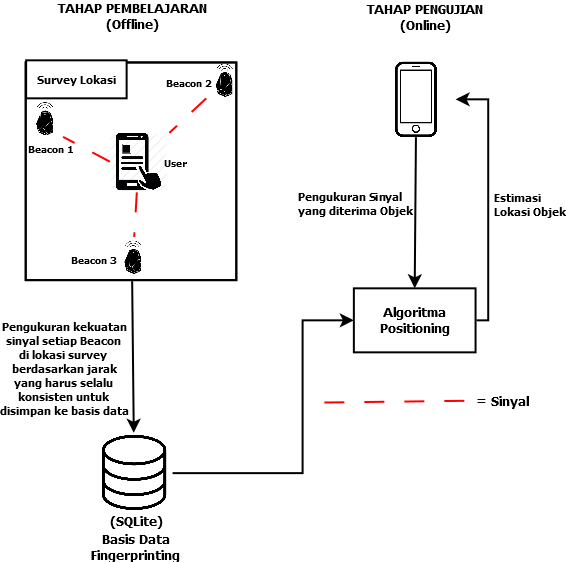
\includegraphics [width = 11cm, height= 9cm]{gambar/fingerprinting}}
	\caption{Ilustrasi Metode \textit{Fingerprinting} }.
	\label{fingerprinting}
\end{figure}

\par Tahap pertama adalah tahap pembelajaran (\textit{offline}), di mana lokasi \textit{Fingerprints} itu sendiri diperoleh dengan cara mengumpulkan RSSI dalam satuan desibel (dBm) yang dipancarkan dari masing-masing AP. Kemudian, gelombang radio akan dipancarkan oleh AP yang diletakkan pada posisi yang telah ditentukan sebelumnya ditangkap oleh \textit{smartphone} dengan kondisi WLAN ataupun Bluetooth dalam keadaan hidup. Selama tahap pembelajaran, lokasi yang tidak diketahui data pembelajarannya kemudian dirujuk sebagai titik referensi estimasi lokasi.
\newline
\par Tahap kedua adalah tahap pengujian (\textit{online}), di mana keakuratan perkiraan posisi objek sangat bergantung pada jumlah titik referensi yang dikumpulkan dalam data pembelajaran. Selama tahap pengujian, sistem harus memberikan informasi lokasi setiap objek berdasarkan data RSSI yang diamati. Namun, nilai RSSI bisa dipengaruhi oleh keadaan lingkungan sekitar yang dapat mengganggu keakuratannya.

\section{\uppercase{\textit{RECEIVED SIGNAL STRENGTH INDICATOR} (RSSI)}}
\textit{Positioning system} menghasilkan data yang penting untuk menghitung lokasi pengguna. \textit{Time of Arrival} (TOA), \textit{Time Difference of Arrival} (TDOA), \textit{Angle of Arrival} (AOA) dan RSSI adalah metode yang sesuai untuk menghitung data lokasi pengguna untuk kasus \textit{positioning system} \citep{Liu2007}. RSSI menunjukkan kekuatan atau daya yang diterima oleh sinyal \citep{Kajioka2014}. RSSI memperkirakan jarak \textit{node} yang belum diketahui ke referensi node dari beberapa kumpulan unit perhitungan dengan menggunakan atenuasi kekuatan sinyal (\textit{signal strength}) yang dipancarkan dari \textit{transmitter}. Metode ini tepat dilakukan dengan frekuensi sinyal radio \citep{Schneegans2007}.

\par Sebuah nilai RSSI didefinisikan dengan bilangan negatif. Semakin tinggi bilangan negatifnya, maka kekuatan sinyal tersebut tergolong lemah. Namun, jika bilangan nilai RSSI mendekati 0, maka kekuatan sinyal tersebut tergolong kuat. Biasanya, jika suatu objek berada di dekat AP atau \textit{transmitter}, RSSI akan memperoleh nilai yang besar. RSSI dapat digolongkan menjadi 5 kategori kekuatan sinyal seperti terlihat pada Tabel \ref{t_rssi}.

\begin{table}[H]
	\centering
	\caption{Kekuatan Sinyal RSSI \citep{VerisIndustries2013}}
	\label{t_rssi}
	\begin{tabular}{|l|l|l|}
		\hline
		\textbf{No.} & \textbf{Kekuatan Sinyal} & \textbf{Kualitas Sinyal} \\
		\hline
		1.           & Kurang dari -40 dB       & Luar Biasa               \\
		\hline
		2.           & -40 dB hingga -55 dB     & Sangat Baik              \\
		\hline
		3.           & -55 dB hingga -70 dB     & Baik                     \\
		\hline
		4.           & -70 dB hingga -80 dB     & Cukup Baik               \\
		\hline
		5.           & Lebih dari -80 dB        & Buruk                    \\
		\hline
	\end{tabular}
\end{table}

\section{\uppercase{\textit{BLUETOOTH LOW ENERGY} (BLE)}}
\par BLE Beacon pada dasarnya adalah sebuah perangkat yang sangat sederhana berupa perangkat wireless kecil yang berbasiskan \textit{Bluetooth Low Energy} yang mentransmisikan sinyal radio secara terus menerus yang berkaitan dengan ID dari beacon tersebut. Dengan menggunakan Smartphone Android terkini, BLE sangat mudah untuk dibaca dan dideteksi. Beberapa informasi yang diperoleh pada pembacaan ini, seperti data sensor dan estimasi jarak antara beacon dengan Smartphone. Hanya dengan kedua data tersebut, developer dapat berkreasi untuk mengembangkan banyak aplikasi yang unik, aplikatif, dan dapat bermanfaat untuk optimasi sistem di industri juga manfaat lainnya \citep{Gupta2016}.

\par Meskipun BLE \textit{beacon} sangat sederhana, namun, BLE \textit{beacon} dibuat dengan teknologi yang cukup maju. Bluetooth Low Energy, yang merupakan media akses dari beacon, memiliki cakupan yang cukup luas (Secara teori 200 m) dari segi jangkauan dibandingkan dengan Wireless Short Range lainnya. Bahkan saat ini dengan berkembangnya \textit{Bluetooth} 5.0, jangkauan \textit{Bluetooth Smart}, menurut Bluetooth SIG, dapat menjangkau 4 kali lipat dibandingkan dengan Bluetooth 4.0. Selain itu, dari sisi low energy, teknologi ini menciptakan interaksi seamless yang tidak mengkonsumsi banyak energy batere (secara teori, dengan batere 3 volt dapat bertahan selama 2 tahun). Selain itu, oleh karena sistem yang tidak kompleks, teknologi beacon tidak perlu bertarung dengan banyak standar aplikasi IoT, sehingga memudahkan developer dalam pengembangannya \citep{Gupta2013}.

\cite{Keluza2017}, mengemukakan bahwa Bluetooth merupakan alat komunikasi tanpa kabel yang digunakan untuk pertukaran data dalam jarak yang dekat. Bluetooth dikembangkan oleh Ericson di tahun 1994. Kemudian di tahun 1998 Ericson, IBM, Intel, Nokia dan Toshiba membentuk wewenang kekuasaan khusus yang dinamakan dengan Bluetooth Interest Group (SIG). Pertengahan tahun 2010, Bluetooth SIG mengumumkan spesifikasi dari Bluetooth 4.0, yang termasuk di dalamnya meliputi \textit{Bluetooth Classic}, \textit{Bluetooth High Speed} dan BLE. BLE terkadang juga bisa dikatakan sebagai “Bluetooth Pintar”. Meskipun BLE dan \textit{Bluetooth Classic} banyak memiliki kesamaan, BLE sebenarnya memiliki fungsionalitas yang sama sekali berbeda dari \textit{Bluetooth Classic}.

\par Keunggulan BLE dibandingkan \textit{Bluetooth Classic} adalah konsumsi daya baterai dan energi listrik dari BLE untuk \textit{transfer} data jauh lebih kecil dibandingkan dengan \textit{Bluetooh Classic}, tetapi dengan jangkauan konektivitas dan kapasitas pengiriman data yang sama \citep{bluetoothsig2010}. Karakteristik dari BLE adalah ukurannya yang sangat kecil, biaya murah, serta konsumsi daya rendah yang bisa digunakan sampai beberapa tahun ke depan dengan menggunakan jenis baterai AAA \citep{Keluza2017}. Menurut \cite{Paganini2015}, terdapat beberapa platform yang mendukung BLE dan platfrom tersebut sudah mendukung Bluetooth 4.0. Beberapa platform tersebut adalah sebagai berikut:
\begin {itemize}
\itemsep0em
\item iOS5+ (lebih dianjurkan iOS7+).
\item Android 4.3+ (perbaikan \textit{bug} merous di 4.4+).
\item Apple OS X 10.6+.
\item Windows 8 (XP, Vista dan Windows 7 hanya mendukung Bluetooth 2.1).
\item GNU/Linux Vanilla BlueZ 4.93+.
\end{itemize}

\section{\uppercase{BEACON}}
\par Pada penelitian kali ini, \textit{beacon} yang digunakan adalah \textit{Beacon}. \textit{Beacon} adalah teknologi \textit{Bluetooth Low-Energy} yang dapat digunakan untuk melakukan push notification atau tracking ketika kita sudah berada di jangkauan sinyalnya. Ketika pengguna melewati area di mana sistem penentuan posisi atau jaringan IoT dengan beacon diatur, beacon terdekat mengirimkan kode dengan pesan ke perangkat seluler mereka. Kemudian, pesan tersebut muncul sebagai pemberitahuan di perangkat seluler pengguna dengan aplikasi seluler pihak ketiga. Ada tiga hal yang harus diperhatikan untuk membuat sistem berbasis beacon ini berfungsi, yaitu setidaknya ada satu perangkat beacon lagi, aplikasi seluler dan tentunya izin pengguna. Untuk mengaktifkan dukungan beacon, ponsel cerdas harus memiliki iOS 7 atau lebih tinggi atau Android 4 atau lebih tinggi. Standar beacon Apple disebut iBeacon, sedangkan Google bernama Eddystone \citep{Kim2014}.

\par BLE memancarkan sinyal dari alat \textit{transmiter} yang beroperasi menggunakan baterai. Alat \textit{transmiter} tersebut disebut dengan Beacon. Beacon merupakan alat pendeteksi lokasi dengan harga yang terjangkau, ukurannya yang kecil, memiliki daya tahan baterai yang cukup lama, dan tidak membutuhkan energi listrik tambahan. Setiap perangkat \textit{smartphone} dan \textit{tablets} yang mendeteksi sinyal dari Beacon, dapat menghitung jarak dan memperkirakan keberadaan lokasi setiap perangkat sekaligus \citep{Keluza2017}.

\par Kelebihan dari penggunaan Beacon diperkirakan bertahan sampai bertahun-tahun hanya dengan energi baterai, serta tahan terhadap debu dan air sesuai dengan standar IP67, dan memiliki ketelitian sejauh 1-3 meter \citep{Insoft2016}. Teknologi BLE merupakan solusi yang tepat yang digunakan pada Beacon, karena penggunaan dayanya yang murah, BLE juga termasuk sistem yang ramah lingkungan. Penggunaan daya yang murah pada BLE dicapai dengan menjaga waktu proses transmisi data sesingkat mungkin dan mengizinkan perangkat \textit{smartphone} maupun \textit{tablets} berada pada mode tidur saat proses transmisi data \citep{Feng2011}.

\section{\uppercase{\textit{SUPPORT VECTOR MACHINE}(SVM)}}
\textit{Support vector machine} (SVM) adalah jenis algoritma klasifikasi \textit{supervised machine learning}. SVM pertama kali diperkenalkan pada 1960-an dan kemudian disempurnakan pada 1990-an. Namun, baru sekarang mereka menjadi sangat populer, karena kemampuan mereka untuk mencapai hasil yang cemerlang. SVM diimplementasikan dengan cara yang unik jika dibandingkan dengan algoritme pembelajaran mesin lainnya \citep{Campbell2010}.

\par Dalam kasus data yang dapat dipisahkan secara linier dalam dua dimensi, seperti yang ditunjukkan pada Gambar \ref{svm1}, algoritma pembelajaran mesin yang khas mencoba menemukan batas yang membagi data sedemikian rupa sehingga kesalahan klasifikasi dapat diminimalkan. Jika Anda melihat lebih dekat pada Gambar \ref{svm1}, mungkin ada beberapa batas yang membagi titik data dengan benar. Dua garis putus-putus serta satu garis padat mengklasifikasikan data dengan benar \citep{Zhibin2008}.

\begin{figure}[H]
	\centering
	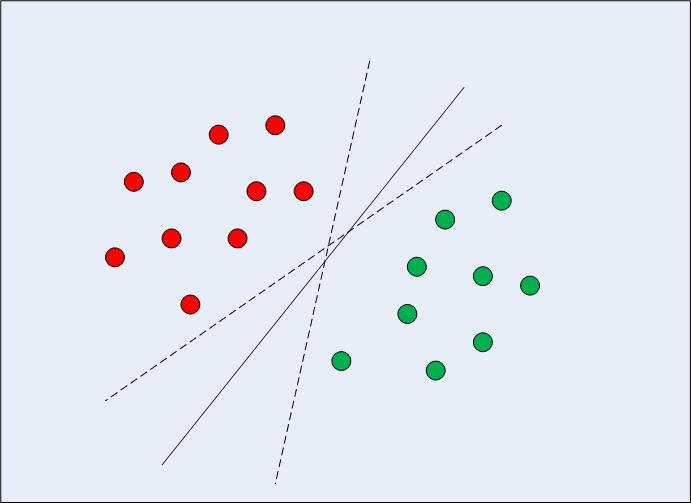
\includegraphics[width=11cm, height=8cm]{gambar/implementing-svm-kernel-svm-python-scikit-learn}
	\caption{Batas Keputusan Ganda.}
	\label{svm1}
\end{figure}

\par SVM berbeda dari algoritma klasifikasi lainnya dalam hal memilih batas keputusan yang memaksimalkan jarak dari titik data terdekat dari semua kelas. SVM tidak hanya menemukan batas keputusan; ia menemukan batas keputusan yang paling optimal.

\par Batas keputusan yang paling optimal adalah batas yang memiliki margin maksimum dari titik terdekat dari semua kelas. Titik terdekat dari batas keputusan yang memaksimalkan jarak antara batas keputusan dan titik disebut support vector seperti terlihat pada Gambar \ref{svm2}. Batas keputusan dalam kasus mesin support vector disebut \textit{maximum margin classifier}, atau \textit{maximum margin hyper plane}.

\begin{figure}[H]
	\centering
	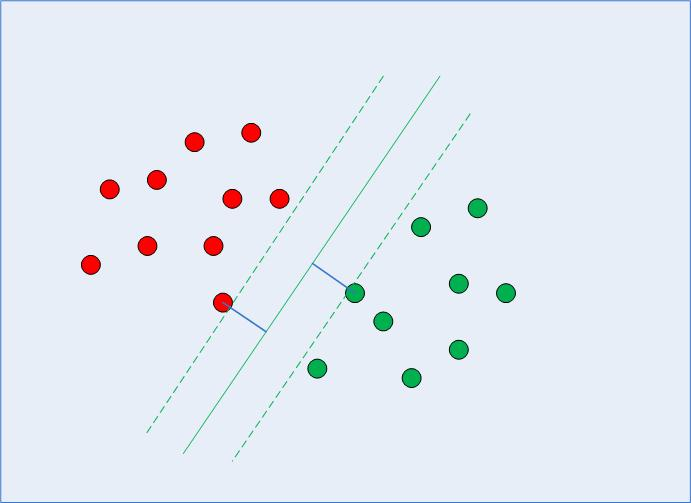
\includegraphics[width=11cm, height=8cm]{gambar/implementing-svm-kernel-svm-python-scikit-learn-2}
	\caption{Batas Keputusan dengan Support Vectors}
	\label{svm2}
\end{figure}

\par Margin (d) = minimum distance antara hyperplane and training samples. Hyperplane terbaik diperoleh dengan memaksimalkan d. Cara memaksimalkan d adalah :
\begin{equation}
	Margin = \frac{2}{|w|^2} = \frac{1-(-1)}{\sqrt{w{1}^2+w{2}}} = \frac{2}{|w|}
\end{equation}

Artinya meminimalkan:
\begin{equation}
	L(w)=\frac{|w|^2}{2}
\end{equation}

\par Umumnya, \textit{Support Vector Machines} dianggap sebagai pendekatan klasifikasi, tetapi dapat digunakan di kedua jenis masalah klasifikasi dan regresi. Itu dapat dengan mudah menangani beberapa variabel kontinu dan kategoris. SVM membangun hyperplane dalam ruang multidimensi untuk memisahkan kelas yang berbeda. SVM menghasilkan hyperplane optimal secara iteratif, yang digunakan untuk meminimalkan kesalahan. Ide inti dari SVM adalah untuk menemukan hyperplane marginal maksimum (MMH) yang paling baik membagi dataset ke dalam kelas \citep{Braun2011}.

\begin{figure}[H]
	\centering
	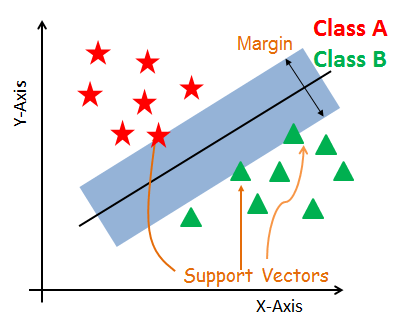
\includegraphics[width=10cm, height=7.3cm]{gambar/index3_souoaz}
	\caption{Support Vectors}
	\label{index3_souoaz}
\end{figure}

\par Support vector adalah titik data yang paling dekat dengan hyperplane. Titik-titik ini akan menentukan garis pemisah lebih baik dengan menghitung margin. Poin-poin ini lebih relevan dengan konstruksi classifier. Hyperplane adalah bidang keputusan yang memisahkan antara satu set objek yang memiliki keanggotaan kelas yang berbeda. Margin adalah jarak antara dua garis pada titik kelas terdekat. Ini dihitung sebagai jarak tegak lurus dari garis untuk mendukung vektor atau titik terdekat. Jika margin lebih besar di antara kelas, maka itu dianggap margin yang baik, margin yang lebih kecil adalah margin yang buruk \citep{Campbell2010}.

\par Tujuan utamanya adalah untuk memisahkan dataset yang diberikan dengan cara terbaik. Jarak antara kedua titik terdekat dikenal sebagai margin. Tujuannya adalah untuk memilih hyperplane dengan margin maksimum yang mungkin antara support vector dalam dataset yang diberikan. SVM mencari hyperplane marginal maksimum dalam langkah-langkah berikut:

\begin{enumerate}[1.]
	\itemsep0em
	\item Generate hyperplanes yang memisahkan kelas dengan cara terbaik. Gambar sisi kiri menunjukkan tiga hyperplanes hitam, biru dan oranye. Di sini, biru dan oranye memiliki kesalahan klasifikasi yang lebih tinggi, tetapi hitam memisahkan dua kelas dengan benar.

	\item Pilih hyperplane kanan dengan segregasi maksimum dari salah satu titik data terdekat seperti yang ditunjukkan pada gambar sisi kanan.
\end{enumerate}

\begin{figure}[H]
	\centering
	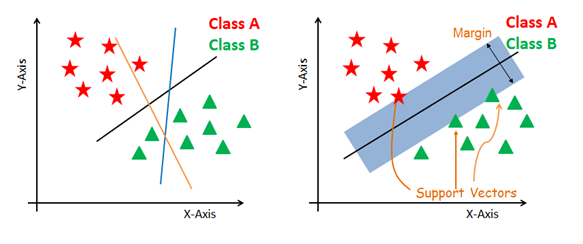
\includegraphics[width=14cm, height=6cm]{gambar/index2_ub1uzd}
	\caption{Support Vectors}
	\label{index3_souoaz}
\end{figure}
\par Beberapa masalah tidak dapat diselesaikan dengan menggunakan hyperplane linier, seperti yang ditunjukkan pada gambar di bawah (sisi kiri). Dalam situasi seperti itu, SVM menggunakan trik kernel untuk mengubah ruang input ke ruang dimensi yang lebih tinggi seperti yang ditunjukkan di sebelah kanan. Titik data diplot pada sumbu x dan sumbu z (Z adalah jumlah kuadrat dari $x$ dan $y$ : $z=x^2=y^2$)

\par Algoritma SVM diimplementasikan dalam praktik menggunakan kernel. Kernel mengubah ruang data input ke dalam bentuk yang diperlukan. SVM menggunakan teknik yang disebut trik kernel. Di sini, kernel mengambil ruang input berdimensi rendah dan mengubahnya menjadi ruang berdimensi lebih tinggi. Dengan kata lain, Anda dapat mengatakan bahwa itu mengubah masalah yang tidak dapat dipisahkan menjadi masalah yang dapat dipisahkan dengan menambahkan lebih banyak dimensi padanya. Hal ini paling berguna dalam masalah pemisahan non-linier. Trik kernel membantu Anda membuat pengklasifikasi yang lebih akurat \citep{Campbell2010}.
\begin{itemize}
	\itemsep0em
	\item Kernel linier dapat digunakan sebagai produk titik normal pada dua pengamatan yang diberikan. Produk antara dua vektor adalah jumlah perkalian dari setiap pasangan nilai input.

	      \begin{equation}
		      K(x, x_{i}) = \sum_{i=1}^{n} (x \times x{i})
	      \end{equation}

	\item Kernel polinomial adalah bentuk yang lebih umum dari kernel linier. Kernel polinomial dapat membedakan ruang input melengkung atau nonlinier.
	      \begin{equation}
		      K(X,X_{i})= 1 + \sum_{i=1}^{n} (X \times X{i})^d
	      \end{equation}

	      Dimana d adalah derajat polinomial. d=1 mirip dengan transformasi linier. Derajat perlu ditentukan secara manual dalam algoritma pembelajaran.

	\item Kernel Fungsi Basis Radial Kernel fungsi basis Radial adalah fungsi kernel populer yang umum digunakan dalam klasifikasi mesin vektor pendukung. RBF dapat memetakan ruang input dalam ruang dimensi tak terbatas.

	      \begin{equation}
		      K(x,x_{i}) = exp(-gamma \times \sum_{i=1}^{n} ((x – x{i}^2))
	      \end{equation}

	      Di sini gamma adalah parameter, yang berkisar dari 0 hingga 1. Nilai gamma yang lebih tinggi akan sangat cocok dengan dataset pelatihan, yang menyebabkan over-fitting. Gamma=0,1 dianggap sebagai nilai default yang baik. Nilai gamma perlu ditentukan secara manual dalam algoritma pembelajaran.
\end{itemize}


\section{\uppercase{ANDROID}}
Android adalah sistem operasi untuk perangkat \textit{smartphone} berbasis Linux \citep{Safaat2011}. Android menyediakan platform \textit{open source} bagi para \textit{developer} untuk menciptakan aplikasi mereka sendiri untuk digunakan oleh bermacam peranti bergerak. Aplikasi Android di tulis dengan bahasa pemrograman Java. Bagaimanapun juga, tanpa menggunakan standar Java Virtual Machine (JVM) sebuah aplikasi Android tidak akan bisa berjalan. Android SDK menyediakan sebuah \textit{tools} dan API untuk mengembangkan sebuah aplikasi pada platform \citep{Sarkar2019}. Menurut \cite{Supardi2011}, ada 4 komponen utama pada aplikasi Android yaitu sebagai berikut:
\begin{enumerate}[1.]
	\itemsep0em
	\item \emph{Activities}, merupakan komponen untuk menyajikan tampilan aplikasi kepada pengguna (\textit{user interface}).
	\item \emph{Service}, merupakan komponen yang tidak memiliki \textit{user interface} atau disebut dengan \textit{layout} pada Android. Namun, \textit{service} ini bekerja dengan cara \textit{background processing}.
	\item \emph{Broadcast Receiver}, merupakan komponen yang berfungsi menerima dan bertugas untuk menyampaikan notifikasi.
	\item \emph{Content Provider}, merupakan komponen yang menangani data secara spesifik sehingga dapat digunakan oleh aplikasi lain.
\end{enumerate}

\section{\uppercase{REACT NATIVE}}
React Native adalah framework JavaScript untuk mengembangkan aplikasi mobile secara multi-platform. Khususnya, pada bagian \textit{front-end} alias interface aplikasi. Sifatnya yang cross-platform memungkinkan satu codebase bisa digunakan di iOS dan Android. Selain itu, React Native juga menghasilkan aplikasi dengan UI/UX mengesankan. Aplikasi bisa berfungsi dengan \textit{smooth} dan komponennya (seperti tombol-tombol) merespon dengan baik layaknya dibuat dengan kode Native \citep{Brito2018}. Cara Kerja React Native cukup simple, yaitu:
\begin{enumerate}[1.]
	\itemsep0em
	\item Developer menggunakan kode React untuk membangun interface aplikasi
	\item Kode React akan diinterpretasikan menjadi JavaScript agar nantinya bisa digunakan untuk aplikasi mobile
	\item React Native akan menggunakan fitur bridge untuk mengolah codebase menjadi Native Module (Android Module, iOS Module)
	\item Native Module siap digunakan di platform yang bersangkutan.
\end{enumerate}

\section{\uppercase{WEB SERVICES}}
\par Web service merupakan aplikasi yang berisi sekumpulan basis data (database) dan perangkat lunak (software) atau bagian dari program perangkat lunak yang diakses secara remote oleh piranti dengan perantara tertentu. Melalui web service, memungkinkan pengguna untuk mengatasi permasalahan berupa interoperability dan mengintegrasikan sistem berbeda \citep{Chuangwei2011}.

\par Pada umumnya, web service memiliki ciri khusus berupa URL layaknya web. Yang membuat berbeda adalah interaksi yang diberikan oleh web service itu sendiri. URL pada web service hanya mengandung sekumpulan informasi, perintah, dan konfigurasi (sintaks yang berguna untuk membangun fungsi tertentu dari aplikasi). Web service mampu menukar data tanpa memandang sumber database, bahasa yang digunakan, dan pada platform apa data tersebut dikonsumsi. Kemampuan itulah yang memungkinkan web service menjadi jembatan penghubung untuk berbagai sistem \citep{Chuangwei2011}.

\par \textit{Web services} menggambarkan aplikasi yang mengekspos \textit{business logic} sebagai layanan yang menggunakan internet \citep{Mironela2009}. Layanan tersebut dikirim melalui \textit{interface} yang dapat diprogram, sementara fungsionalitasnya dapat dipakai dan dipanggil melalui alamat \textit{Internet Protocol} (IP \textit{address}) \citep{Wagh2012}. \textit{Web services} sering dikategorikan sebagai komponen sistem perangkat lunak yang dirancang untuk mendukung interaksi antar sistem. \textit{Web services} menyediakan informasi atau data kepada sistem lain untuk digunakan sebagai fasilitas yang membuat sistem dapat saling berinteraksi. Biasanya, data yang diberikan oleh \textit{web services} berupa data dalam bentuk format JavaScript Object Notation (JSON) atau eXtensible Markup Language (XML) \citep{Rahman2013}. Situs \textit{web} World Wide Web Consortium (W3C) mendeskripsikan  bahwa \textit{Simple Object Access Protocol} (SOAP), \textit{Representatonal State Transfer} merupakan protokol yang digunakan \textit{web services} untuk berkomunikasi. Penelitian ini akan menggunakan \textit{web services} dengan layanan protokol REST untuk membantu aplikasi absensi perkuliahan berbasis Android berinteraksi dengan \textit{database} yang terdapat di server.

\section{\uppercase{REPPRESENTATIONAL STATE TRANSFER (REST)}}
REST merupakan hubungan antara klien dan server dan bagaimana sebuah data disimpan. Arsitektur REST didasarkan pada gaya arsitektur klien atau server yang dapat dilihat pada Gambar \ref{restful}. \textit{Request} dan \textit{response} dibangun berdasarkan sumber daya pada saat proses transfer \citep{HaliliRamadani2018}. Konsep dari REST adalah perpindahan antar \textit{state}, dapat dicontohkan seperti sebuah browser yang melakukan permintaan terhadap sebuah halaman situs, maka server akan mengirimkan \textit{state} dari halaman situs tersebut ke browser \citep{Rahman2013}.
\begin{figure}[H]
	\centering
	\shadowbox
	{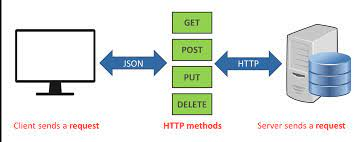
\includegraphics [width = 11cm, height= 4cm]{gambar/restful.jpg}}
	\caption
	{Ilustrasi Arsitektur RESTful dan Komunikasi Antara Klien dan Server \citep{HaliliRamadani2018}}.
	\label{restful}
\end{figure}
\par Navigasi REST dilakukan melalui HTTP untuk melakukan aktivitas tertentu, seolah-olah terjadi perpindahan \textit{state} antara satu halaman dengan halaman lainnya \citep{Rahman2013}. Sebuah aplikasi \textit{web} yang bergantung dengan layanan REST arsitektur disebut dengan RESTful \textit{web services}. RESTful \textit{web services} menggunakan 4 perintah HTTP untuk \textit{create}, \textit{read}, \textit{update} dan \textit{delete} yaitu \textit{GET}, \textit{POST}, \textit{PUT} dan \textit{DELETE} seperti yang terlihat pada Gambar \ref{httprestful} \citep{sinha2014}.
\begin{figure}[H]
	\centering
	\shadowbox
	{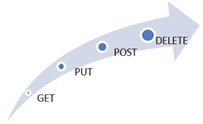
\includegraphics [width = 5cm, height= 3cm]{gambar/httprestful}}
	\caption{Perintah HTTP RESTful \citep{sinha2014}}.
	\label{httprestful}
\end{figure}

\section{\uppercase{SCRUM}}

\par Scrum adalah metode pengembangan perangkat lunak \textit{agile} yang dikembangkan oleh Jeff Sutherland dan tim pengembangannya di awal 1990-an. Selanjutnya, pengembangan lebih lanjut tentang metode Scrum telah dilakukan oleh Schwaber dan Beedle Prinsip scrum konsisten dengan manifesto agile dan digunakan untuk memandu kegiatan pengembangan dalam suatu proses yang menggabungkan kegiatan kerangka kerja (\textit{framework activity}) berikut: kebutuhan (\textit{requirements}), analisis (\textit{analysis}), desain (\textit{design}), evolusi (\textit{evolution}), dan pengiriman (\textit{delivery}). Dalam setiap kegiatan kerangka kerja, \textit{work task} terjadi dalam pola proses yang disebut \textit{sprint}. Pekerjaan yang dilakukan dalam \textit{sprint} (jumlah \textit{sprint} yang diperlukan untuk setiap kegiatan kerangka kerja akan bervariasi tergantung pada kompleksitas dan ukuran produk) disesuaikan dengan masalah yang dihadapi dan didefinisikan dan sering dimodifikasi secara real time oleh tim Scrum \citep{Ereiz2019}.

\par \textit{Scrum} pada dasarnya didasari oleh proses model \textit{Incremental} yang merupakan salah satu model pengembangan perangkat lunak. Dalam metode \textit{Scrum}, seluruh \textit{development cycle} terbagi menjadi sebuah rangkaian iterasi di mana setiap iterasi tersebut merupakan detak jantung dari \textit{Scrum} itu sendiri yang disebut dengan “\textit{Sprint}”. Pengerjaan \textit{Sprint} memiliki durasi maksimal selama 30 hari. Karena durasi \textit{Sprint} lebih singkat dibandingkan dengan durasi pengembangan produk, maka dalam produk \textit{development cycle} akan ada beberapa \textit{Sprint}, yang artinya pengembangan produk dengan metode \textit{Scrum} dilakukan secara \textit{Iterative} dan \textit{Incremental} \citep{Mundra2013}. Tahapan-tahapan metode \textit{Scrum} menurut \cite{Schwab2013} adalah sebagai berikut:
\begin {enumerate}[1.]
\item Dimulai dengan mengumpulkan \textit{user requirements}, namun tidak harus semua \textit{requirements} diharapkan harus keluar dari pemikiran \textit{user} di tahap awal proses pengembangan. \textit{User} dapat mengubah pikiran mereka di setiap waktu selama proses pengembangan, \textit{user} dapat menambah fitur-fitur baru, menghapus atau memperbarui beberapa fitur yang telah ada sebelumnya.
%%%%%%%%%%%%%%%%%%%%%%%%%%%%%%%%%%%%%%%%%%%%%%%%%%%%%%%%%%%%%%%%%%%%%%%%%%%%%%%%%%%%%%%%%%%%%%%%%%%%%%%%%
\item Tahapan selanjutnya adalah memprioritaskan \textit{requirements} dan \textit{Product Backlog}. Sebuah perencanaan yang tepat dalam \textit{Sprint} harus dilakukan sesuai jumlah \textit{Sprint} yang dibutuhkan untuk mengembangkan perangkat lunak, yang terdiri dari durasi \textit{Sprint} tersebut dan \textit{requirements} apa saja yang terdapat di \textit{Product Backlog} yang harus diimplementasikan di setiap \textit{Sprint} (dikenal dengan \textit{Sprint Backlog}).
%%%%%%%%%%%%%%%%%%%%%%%%%%%%%%%%%%%%%%%%%%%%%%%%%%%%%%%%%%%%%%%%%%%%%%%%%%%%%%%%%%%%%%%%%%%%%%%%%%%%%%%%%
\item \textit{Sprint} diawali dengan \textit{Sprint Planning} dimana \textit{Product Owner}, satu orang yang telah diberikan wewenang dan bertanggung jawab untuk memaksimalkan nilai produk di pasar, bertemu dengan tim \textit{Scrum} (tim dengan jumlah 2-9 orang), kemudian bekerja sama untuk memperkirakan \textit{requirements} dari \textit{Product Backlog} apa saja yang dikerjakan selama satu \textit{Sprint}.
%%%%%%%%%%%%%%%%%%%%%%%%%%%%%%%%%%%%%%%%%%%%%%%%%%%%%%%%%%%%%%%%%%%%%%%%%%%%%%%%%%%%%%%%%%%%%%%%%%%%%%%%% 
\item \textit{Sprint Planning} difasilitasi dengan \textit{Scrum Master}. \textit{Scrum Master} adalah seorang pemimpin yang melayani (\textit{Servant Leader}). \textit{Sprint Planning} memiliki batasan waktu selama 8 jam di dalam sebuah \textit{Sprint} yang berdurasi selama 30 hari. Keluaran dari \textit{Sprint Planning} adalah daftar pekerjaan dari hasil kesepakatan antara \textit{Product Owner} dan tim \textit{Scrum} dimana pekerjaan itu yang akan dikerjakan oleh tim \textit{Scrum} nantinya selama satu \textit{Sprint} beserta \textit{Sprint Goal} yang dinamakan dengan \textit{Sprint Backlog}.
%%%%%%%%%%%%%%%%%%%%%%%%%%%%%%%%%%%%%%%%%%%%%%%%%%%%%%%%%%%%%%%%%%%%%%%%%%%%%%%%%%%%%%%%%%%%%%%%%%%%%%%%%
\item Setelah \textit{Sprint Planning} berakhir, tim \textit{Scrum} akan mengambil \textit{Sprint Backlog} untuk diri mereka masing-masing dan mengerjakan \textit{Sprint Backlog} setiap hari hingga akhir \textit{Sprint} tanpa campur tangan dari pihak manapun. \textit{Daily Scrum} akan dikerjakan oleh tim \textit{Scrum} yang tidak lebih dari 15 menit untuk menentukan apa saja yang akan mereka kerjakan selama 24 jam ke depan berdasarkan perkembangan 24 jam terakhir, serta menyampaikan permasalahan yang menghambat mereka untuk bisa mencapai \textit{Sprint Goal}. Tim \textit{Scrum} akan melakukan perbaikan-perbaikan item dari \textit{Product Backlog} pada \textit{Sprint} yang akan datang selama proses pengembangan berlangsung, dengan tujuan membuat \textit{Sprint Planning} menjadi lebih efektif.
%%%%%%%%%%%%%%%%%%%%%%%%%%%%%%%%%%%%%%%%%%%%%%%%%%%%%%%%%%%%%%%%%%%%%%%%%%%%%%%%%%%%%%%%%%%%%%%%%%%%%%%%%
\item Di akhir \textit{Sprint} saat acara \textit{Sprint Review}, \textit{Product Owner} akan mempresentasikan hasil pekerjaan tim \textit{Scrum} selama satu \textit{Sprint} dan juga menjelaskan apa saja pencapaian tim \textit{Scrum} menuju \textit{Sprint Goal} di dalam \textit{Sprint} tersebut kepada para pemegang kepentingan (\textit{stakeholder}) agar mendapatkan \textit{feedback}. \textit{Feedback} ini akan dimasukkan ke dalam \textit{Product Backlog} agar meningkatkan nilai dari sebuah produk. \textit{Sprint Review} memiliki batasan waktu tidak lebih dari 4 jam untuk \textit{Sprint} yang memiliki durasi selama 30 hari.
%%%%%%%%%%%%%%%%%%%%%%%%%%%%%%%%%%%%%%%%%%%%%%%%%%%%%%%%%%%%%%%%%%%%%%%%%%%%%%%%%%%%%%%%%%%%%%%%%%%%%%%%%
\item Setelah \textit{Sprint Review}, \textit{Scrum Master} memfasilitasi acara yang bernama \textit{Sprint Retrospectives} agar tim \textit{Scrum}, \textit{Product Owner} bekerja sama menentukan apa saja peningkatan yang akan mereka implementasikan di \textit{Sprint} berikutnya. \textit{Scrum Master} yang efektif, akan kreatif dalam memfasilitasi \textit{Sprint Retrospectives}, akan masuk ke dalam \textit{Sprint Backlog} untuk menuju \textit{Sprint} berikutnya. \textit{Definition of Done} adalah salah satu hal yang ditekankan oleh tim \textit{Scrum} pada saat \textit{Sprint Retrospectives}.
%%%%%%%%%%%%%%%%%%%%%%%%%%%%%%%%%%%%%%%%%%%%%%%%%%%%%%%%%%%%%%%%%%%%%%%%%%%%%%%%%%%%%%%%%%%%%%%%%%%%%%%%%
\item \textit{Sprint Retrospectives} merupakan acara yang paling penting dalam \textit{Scrum} dikarenakan sifatnya yang menekankan \textit{continuous learning} yang dapat meningkatkan tingkat \textit{agility} perusahaan. \textit{Sprint Review} memiliki batasan waktu tidak lebih dari 3 jam untuk \textit{Sprint} yang memiliki durasi selama 30 hari. Setelah \textit{Sprint Retrospectives} berakhir, maka \textit{Sprint} berikutnya akan langsung dilakukan tanpa ada jeda antar \textit{Sprint}. Pada setiap \textit{Sprint}, \textit{Product Owner} akan memastikan agar produk dapat mencapai nilai setinggi mungkin saat pengembangan produk diakhiri. \textit{Product Owner}, \textit{Scrum Master} dan tim \textit{Scrum} memegang komitmen, keberanian, saling menghargai satu sama lain, keterbukaan dan fokus. Ilustrasi tahapan-tahapan metode Scrum dapat dilihat pada Gambar \ref{scrum} dibawah ini.
\end{enumerate}

\vspace{0,2cm}
\begin{figure}[H]
	\centering
	\shadowbox
	{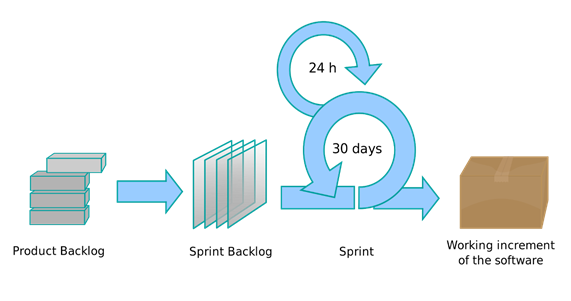
\includegraphics [width = 11cm, height= 5.5cm]{gambar/imagescrum}}
	\caption{Ilustrasi Metode Pengembangan Menggunakan \textit{Scrum} \citep{Schwab2013}}.
	\label{scrum}
\end{figure}


\section{\uppercase{BLACK BOX TESTING}}
Pengujian \textit{black-box} adalah metode pengujian perangkat lunak yang memeriksa fungsionalitas aplikasi tanpa mengintip ke dalam struktur atau cara kerja internalnya. Metode pengujian ini dapat diterapkan secara virtual ke setiap tingkat pengujian perangkat lunak: unit, integrasi, sistem, dan penerimaan. Kadang-kadang disebut sebagai pengujian berbasis spesifikasi. \textit{Black box testing} menurut \citep{Mustaqbal2015} cenderung menemukan hal-hal berikut:
\begin{enumerate}[1.]
	\item Fungsi yang tidak benar atau tidak ada.
	\item Kesalahan \textit{user interface}.
	\item Kesalahan pada struktur data dan akses \textit{database}.
	\item Kesalahan performansi.
	\item Kesalahan inisialisasi dan terminasi.
\end{enumerate}

\section{\uppercase{USABILITY TESTING}}
\par Pengujian kegunaan adalah teknik yang digunakan dalam desain interaksi yang berpusat pada pengguna untuk mengevaluasi suatu produk dengan mengujinya pada pengguna. Ini dapat dilihat sebagai praktik kegunaan yang tak tergantikan, karena memberikan masukan langsung tentang bagaimana pengguna sebenarnya menggunakan sistem. Ini lebih peduli dengan intuitif desain produk dan diuji dengan pengguna yang tidak memiliki paparan sebelumnya. Pengujian tersebut sangat penting untuk keberhasilan produk akhir sebagai aplikasi yang berfungsi penuh yang menciptakan kebingungan di antara penggunanya tidak akan bertahan lama.Ini berbeda dengan metode pemeriksaan kegunaan di mana para ahli menggunakan metode yang berbeda untuk mengevaluasi antarmuka pengguna tanpa melibatkan pengguna.
\citep{Wahl2000}.  \citep{Wesfix2017}.

\par Tujuan lain dilakukannya pengujian ini adalah untuk mengumpulkan data kualitatif yang berhubungan dengan kepuasan pengguna dengan produk yang diuji. Data kualitatif tersebut terdiri dari komentar yang dibuat oleh partisipan, jawaban dari kuisioner pertanyaan dan tanggapan dari partisipan saat proses wawancara. \textit{Usability testing} telah terbukti dapat mengurangi waktu tahap pengembangan, mengurangi jumlah \textit{bugs}, dan menghasilkan produk yang lebih berkualitas untuk meningkatkan nilai jual \citep{Wahl2000}.

\subsection{System Usablity Scale (SUS)}
Metode pengujian dengan \textit{usablity testing} yang digunakan pada penelitian ini adalah SUS. System Usability Scale (SUS) menyediakan alat yang "cepat dan kotor", andal untuk mengukur kegunaan. Ini terdiri dari 10 item kuesioner dengan lima pilihan respon untuk responden; dari Sangat setuju hingga Sangat tidak setuju. Awalnya dibuat oleh John Brooke pada tahun 1986, ini memungkinkan Anda untuk mengevaluasi berbagai macam produk dan layanan, termasuk perangkat keras, perangkat lunak, perangkat seluler, situs web, dan aplikasi.

\par Skala penilaian yang digunakan yaitu skala likert antara 1-5. \cite{Sugiyono2004} mengatakan bahwa skala likert digunakan untuk mengukur pendapat, persepsi dan sikap seseorang atau sekelompok orang tentang fenomena sosial. SUS bertujuan untuk mengetahui penilaian subjektif yang dilakukan dalam pengujian oleh beberapa responden dan meminta pendapat mengenai aplikasi yang akan dibuat pada penelitian ini.

\par Pengujian ini memerlukan kuesioner sebagai teknik pengumpulan informasi pengujian yang didapat dari responden mengenai aplikasi. Kuesioner terdiri dari 10 soal yang terdiri dari pertanyaan positif dan negatif. Pertanyaan positif terdapat pada nomor ganjil (1, 3, 5, 7, 9) dan pertanyaan negatif terdapat pada nomor genap (2, 4, 6, 8, 10). Setiap pertanyaan diberi bobot antara 0-4. Pertanyaan ganjil skor dihitung dengan cara bobot tiap pertanyaan ($x_{i}$) dikurangi 1 (ditulis $x_{i}$ - 1). Sedangkan pertanyaan genap skor dihitung dengan cara 5 dikurangi bobot tiap pertanyaan ($x_{i}$)(ditulis 5 - $x_{i}$) \citep{Ardiansyah2016}. Setiap pertanyaan memiliki 5 pilihan jawaban yang terdiri dari: sangat tidak setuju, tidak setuju, biasa saja, setuju dan sangat setuju.

%\par Rumus menghitung skor pengujian \textit{usability testing} adalah sebagai berikut:
%\begin{equation}
%\overline{x}=\frac{\sum x}{n}
%\end{equation}
%\newline
%Keterangan:\newline
%$\overline{x}$ = skor rata-rata. \newline
%$\sum x$ = jumlah skor SUS. \newline
%$n$ = jumlah responden. 

\subsection{Test Plan}
\textit{Test plan} adalah dokumen yang melibatkan semua anggota tim \textit{developer} untuk melihat apakah fungsionalitas dari produk yang dibuat sudah terpenuhi atau belum. Dengan kata lain, \textit{test plan} disebut sebagai tujuan, perencanaan atau skenario untuk melakukan \textit{testing} yang akan dilakukan baik itu \textit{expert} \textit{user} atau \textit{user} awam. \textit{Test plan} perlu dibuat saat melakukan pengujian karena \textit{test plan} menggambarkan bagaimana cara menguji produk tersebut. \textit{Test plan} memaksa untuk melakukan pengujian secara sistematis \citep{Rubin2008}. Bagian-bagian dari \textit{test plan} menurut \cite{Rubin2008} adalah sebagai berikut:
\begin{itemize}
	\item Maksud, tujuan dan sasaran pengujian.
	\item Pertanyaan terkait penelitian.
	\item Karakteristik partisipan.
	\item Metode yang digunakan (\textit{test design}).
	\item \textit{List} tugas.
	\item Lingkungan pengujian, perlengkapan, dan logistik.
	\item Peran moderator pengujian.
	\item Data yang dikumpulkan dan langkah-langkah evaluasi.
	\item Laporan dan presentasi.
\end{itemize}








%-----------------------------------------------------------------------------%

% Baris ini digunakan untuk membantu dalam melakukan sitasi
% Karena diapit dengan comment, maka baris ini akan diabaikan
% oleh compiler LaTeX.
\begin{comment}
\bibliography{daftar-pustaka}
\end{comment}


  %-------------------------------------------------------------------------------
%                            BAB III
%               		METODOLOGI PENELITIAN
%-------------------------------------------------------------------------------
\fancyhf{}
\fancyfoot[C]{\thepage}
\chapter{METODOLOGI PENELITIAN}

\section{\uppercase{WAKTU DAN LOKASI PENELITIAN}}
\setlength\parindent{30pt} Penelitian ini dilaksanakan di lantai 1 dan 3 di Gedung A FMIPA Universitas Syiah Kuala (USK). Waktu yang dibutuhkan untuk penelitian ini adalah 5 bulan terhitung dari bulan May 2021 hingga Oktober 2021.

\section{\uppercase{ALAT DAN BAHAN}}
Alat dan bahan yang digunakan pada penelitian ini meliputi perangkat keras, perangkat lunak dan bahan yang mendukung pada penelitian ini adalah data \textit{Received Signal Strength Indicator} (RSSI) dari hasil survei di lokasi penelitian. Adapun perangkat lunak yang digunakan adalah:
\begin{itemize}
	\itemsep0em
	\item OS Windows 10.
	\item Google Chrome.
	\item Visual Studio Code 1.59.1
	\item React Native
	\item MongoDB Compass 1.28.1
	\item Figma
	\item Postman 8.12.0
\end{itemize}

\par Sedangkan komponen perangkat keras yang digunakan meliputi 1 unit Laptop Acer dengan RAM 3GB, Intel® Core™ i3-3230M CPU @2.60Ghz (4 CPUs), ~2.6 GHz Processor, \textit{Harddisk} 500GB, \textit{Solid State Drive} (SSD) 120GB, memiliki Sistem Operasi Windows 64-bit, 20 unit \textit{KBeacon}, serta smartphone Samsung A30.

\section{\uppercase{METODE PENELITIAN}}
Metode penelitian yang dilakukan terdiri dari beberapa tahapan. Skema dari alur tahapan tersebut dapat dilihat pada Gambar \ref{metpen}.
\begin{figure}[H]
	\centering
	{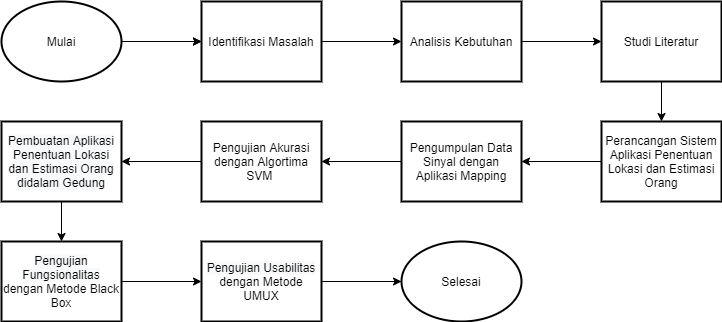
\includegraphics [width = 14cm, height= 6cm]{gambar/metodepenelitian.drawio }}
	\caption{Diagram Alir Penelitian}
	\label{metpen}
\end{figure}

\fancyhf{}
\fancyfoot[R]{\thepage}

\subsection{Identifikasi Masalah}
Tahapan ini adalah proses mengidentifikasi masalah sehingga aplikasi ini perlu dibuat. Adapun masalah yang diidentifikasikan adalah sebagai berikut:
\begin{enumerate}[1.]
	\itemsep0em
	\item Global Positioning System (GPS) belum bisa berfungsi jika digunakan dalam gedung.
	\item Pengguna buta arah perlunya petunjuk arah di dalam gedung
	      \citep{Keluza2017}.
	\item Perlunya data estimasi orang dalam gedung untuk pencegahan Covid-19
	\item Aplikasi untuk \textit{mapping} menyimpan data di local device sehingga tidak dapat dilakukan dengan banyak device sekaligus.
	\item Belum tersedia Aplikasi Penentuan Lokasi dan Estimasi Orang dalam Gedung .
\end{enumerate}

%%%%%%%%%%%%%%%%%%%%%%%%%%%%%%%%%%%%%%%%%%%
\subsection{Analisis Kebutuhan}
Pada tahapan ini, analisa kebutuhan bersumber dari masalah yang telah diidentifikasi pada tahap sebelumnya sehingga perancangan aplikasi dibangun sesuai kebutuhan. Adapun kebutuhan dari sistem yang dibangun adalah sebagai berikut:

\par \textbf{Kebutuhan Fungsional} Kebutuhan fungsional adalah fungsionalitas sistem itu sendiri. Adapun kebutuhan fungsional dari identifikasi masalah yang telah dilakukan adalah sebagai berikut:

\begin{itemize}
	\item Melakukan proses penentuan lokasi pengguna di dalam gedung FMIPA USK berbasis Crowdsourcing Indoor Localization System.

	\item Menampilkan prediksi lokasi pengguna saat berada di dalam gedung FMIPA USK.

	\item Menampilkan data estimasi orang di dalam gedung FMIPA USK.

\end{itemize}

\par \textbf{Kebutuhan Non-Fungsional} Kebutuhan non-fungsional memastikan batasan eksternal yang harus dipenuhi oleh sistem. Batasan-batasan tersebut antara lain:
\begin{itemize}
	\item System hanya dapat mendeteksi lokasi pengguna di dalam gedung yang telah dipetakan

	\item Dapat melakukan proses penentuan lokasi apabila bluetooth pada perangkat hidup dan terkoneksi dengan internet.

	\item Dapat mendata estimasi orang di dalam gedung.

\end{itemize}



%%%%%%%%%%%%%%%%%%%%%%%%%%%%%%%%%%%%%%%%%
\subsection{Studi Literatur}
Pada proses studi literatur, peneliti mengumpulkan bahan referensi penelitian yang bersumber dari jurnal-jurnal nasional dan internasional yang terkait penelitian ini dan situs \textit{website} serta buku-buku referensi untuk penelitian ini. Studi literatur dikembangkan untuk menyempurnakan penelitian sebelumnya.

\subsection{Perancangan Sistem}
Pada tahap ini, peneliti merancang alur kerja  sistem sehingga bisa memastikan sistem yang dirancang dapat digunakan sesuai kebutuhan pengguna. Alur kerja sistem dijelaskan menggunakan diagram alir yang dapat dilihat dari gambar berikut ini.
\ref{alur-kerja-sistem}.

\begin{figure}[H]
	\centering
	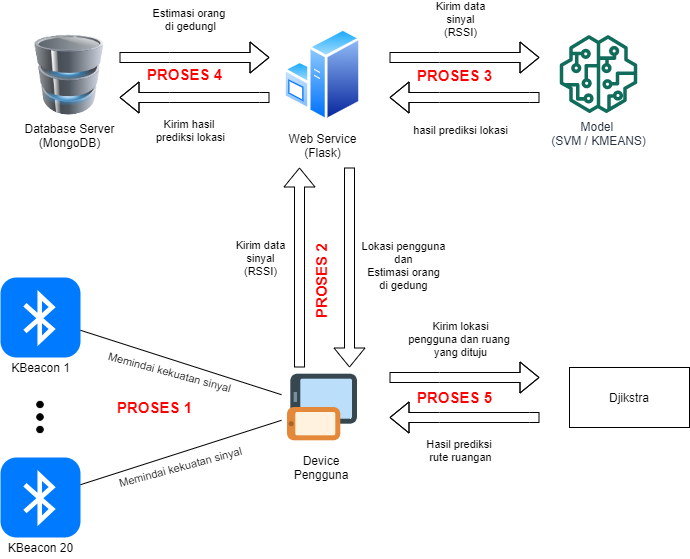
\includegraphics[width=10cm, height=8cm]{gambar/perancangansistem.png}
	\caption{Alur Kerja Sistem.}
	\label{alur-kerja-sistem}
\end{figure}

\subsection{Pembuatan Sistem}
Metode yang digunakan pada sistem ini adalah metode \textit{Scrum}. Metode \textit{Scrum} merupakan metodologi yang termasuk dalam agile software development. \textit{Scrum} dinilai dapat menghasilkan kualitas perangkat lunak yang baik sesuai dengan keinginan pengguna, dapat digunakan dalam proyek besar maupun kecil, dan mudah untuk mengadopsi perubahan.Sistem ini memiliki empat aplikasi yang terdiri dari tiga aplikasi utama dan satu aplikasi pendukung. yaitu:
\begin{enumerate}
	\item Aplikasi Penentuan Lokasi dan Estimasi Jumlah Orang
	      \newline Aplikasi ini merupakan aplikasi utama yang berfungsi untuk melakukan proses penentuan lokasi dan estimasi jumlah orang yang berada di dalam gedung A Fakultas Matematika dan Ilmu Pengetahuan Alam USK. Aplikasi ini dibangun menggunakan framework \textit{React native}

	\item Aplikasi \textit{Web Service Flask} Untuk Menjalankan Model \textit{Support Vector Machine} (SVM)
	      \newline Aplikasi \textit{Web Service Flask} merupakan aplikasi utama, yang mana aplikasi \textit{Web Service Flask} ini akan menjalankan model yang telah dihasilkan oleh kode bahasa \textit{python}.

	\item Aplikasi \textit{Mapping}
	      \newline Aplikasi ini merupakan aplikasi pendukung yang berfungsi untuk melakukan pengumpulan data. Data yang dikumpulkan berupa data kekuatan sinyal RSSI berdasarkan lokasi dimana data tersebut diambil. Setelah pengumpulan data selesai dilakukan, data tersebut akan di kirim ke \textit{Web Service GraphQL} dan kemudian akan di simpan ke \textit{Database MongoDB}.

	\item Aplikasi \textit{Web Service GraphQL} Untuk Menyimpan Data \textit{Mapping}
	      \newline Aplikasi \textit{Web Service GraphQL} merupakan aplikasi pendukung, yang mana aplikasi \textit{Web Service GraphQL} ini akan menyimpan data \textit{mapping} RSSI yang dikirimkan oleh \textit{device} peneliti.

\end{enumerate}

\subsection{Pengembangan Aplikasi Mapping}
\par Untuk memperoleh dataset untuk penelitian ini, maka diperlukan aplikasi \textit{mapping} untuk menangkap sinyal \text{bluetooth} dari alat \textit{Beacon}. Nilai RSSI yang diperoleh dari 20 \textit{Beacon} yang dipasang dari setiap sudut ruangan akan disimpan dalam database mongoDB. Pada penelitian sebelumnya, aplikasi \textit{mapping} menyimpan data di local server sehingga  tidak efektif jika digunakan oleh banyak server. Oleh karena itu, penulis merancang \textit{Web Service} agar data yang disimpan saat penelitian atau \textit{mapping} akan disimpan di database \textit{mongoDB}. Adapun fitur yang tersedia pada aplikasi \textit{mapping} ini adalah:

\begin {itemize}
\itemsep0em
\item Pemindaian Kekuatan Sinyal \newline
Aplikasi ini akan melakukan pemindaian kekuatan sinyal yang ditangkap dari setiap \textit{beacon} yang ditempel di setiap sudut ruangan, sehingga bisa menampilkan data RSSI, label, \textit{Mac Address}, nama \textit{beacon} yang ditandai tersebut.

\item Menyimpan Data Kekuatan Sinyal \newline
Ketika selesai melakukan \textit{mapping}, data kekuatan sinyal disimpan ke database \textit{mongoDB} yang berada di server. Data tersebut akan digunakan pada tahap penelitian selanjutnya.

\end{itemize}

%%%%%%%%%%%%%%%%%%%%%%%%%%%%%%%%%%%%%%%%%%%%%%%%%%%%%%%%%%%%%%%%%%%%%%%%%%%%%%%%%%%%%%%%%%%%%%%%%%%%%%%%%%%%%%%%%%
\subsection{Pengumpulan Data}
\begin{enumerate}[a.]
	\itemsep0em
	\item Pembuatan Denah Lokasi Penelitian
	      \\
	      Pembuatan Denah Lokasi Penelitian didasarkan pada rancangan gedung FMIPA USK. Denah ini dapat digunakan untuk menentukan posisi \textit{reference point} untuk proses pemetaan nantinya. Proses penentuan letak \textit{reference point} ini dilakukan dengan cara menghitung luas lokasi penelitian.
	      %%%%%%%%%%%%%%%%%%%%%%next%%%%%%%%%%%%%%%%%%%%%

	\item Pengukuran Jarak Lokasi Penelitian
	      \\
	      Pengukuran ini bertujuan untuk mengukur jarak dari denah lokasi penelitian yang telah dibuat. Hal ini agar bertujuan untuk membuat bobot pada algoritma \textit{Support Vector Machine} (SVM).

	\item Penentuan Letak \textit{Reference Point}
	      \\
	      Pada tahap ini, letak \textit{reference point} berada di gedung Blok A FMIPA USK, diantaranya adalah di lantai 1, tangga lantai 1 menuju lantai 2, tangga lantai 2 menuju lantai 3, koridor depan Laboratorium Jaringan Komputer, Laboratorium Database, dan Laboratorium Sistem Informasi Geografis.Penentuan letak \textit{reference point} ini dilakukan di setiap sudut ruangan kecuali di dalam ruangan laboratorium. Penentuan \textit{reference point} dilakukan secara urut dengan masing-masing jarak antara satu \textit{reference point} ke \textit{reference point} yang lain sejauh 2 ubin lantai atau 120 centimeter untuk meminimalisir \textit{position error}. \citep{Lee2019} \citep{Bahl2000}. Tujuan penentuan posisi \textit{reference point} ini bertujuan untuk menentukan lokasi pengumpulan data kekuatan sinyal yang dipancarkan setiap \textit{Beacon} di setiap sudut ruangan. Penentuan \textit{reference point} yang saling berdekatan mempengaruhi hasil tahap \textit{positioning}. Denah lokasi penelitian ini dapat dilihat pada Gambar \ref{gedungA}.

	      %\vspace{2cm}
	      \begin{figure}[H]
		      \centering
		      \subfloat[Denah Lantai 1]{{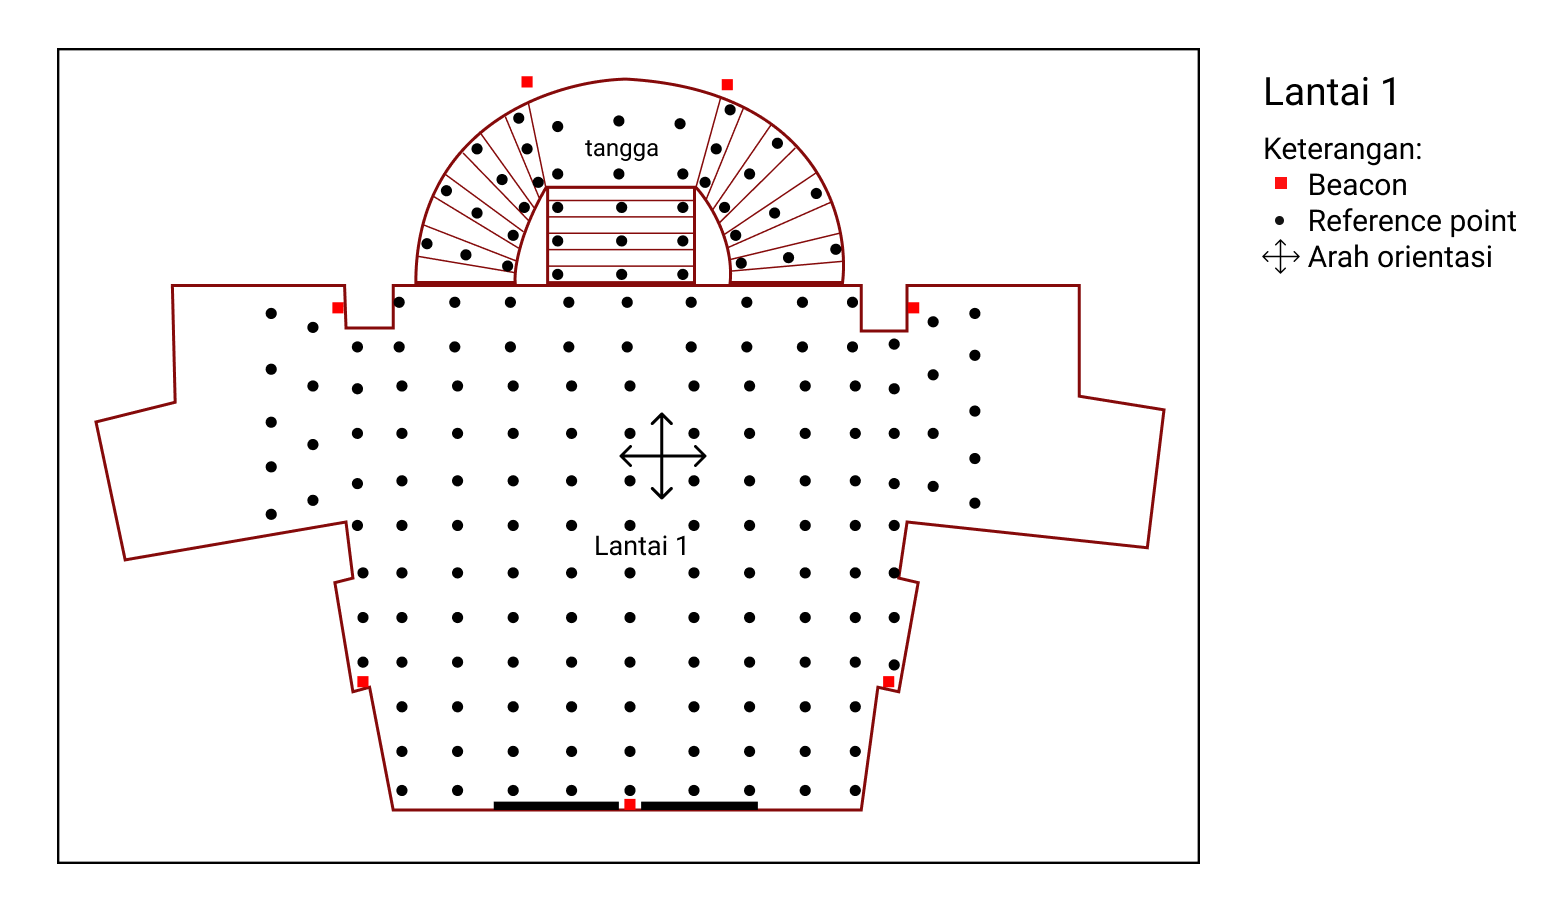
\includegraphics[width=13cm, height=7cm]{gambar/Lantai1} }}%
		      \qquad
		      \subfloat[Denah Lantai 2]{{\includegraphics[width=13cm, height=8cm]{gambar/lantai2} }}

		      \centering
		      \subfloat[Denah Lantai 3]{{\includegraphics[width=12cm, height=6cm]{gambar/lantai3} }}
		      \caption{Ilustrasi Denah Lokasi Letak \textit{Reference Point} Penelitian Gedung Blok A FMIPA}%
		      \label{gedungA}%
	      \end{figure}

	      \par Pada proses ini, masing-masing \textit{reference point} saat mengambil kekuatan sinyal akan menghadap 4 arah oriental yaitu depan, belakang, kiri dan kanan.Kekuatan sinyal pada lokasi tertentu memiliki nilai yang bervariasi hingga -5 dBm tergantung orientasi yang dihadapi pengguna \cite{Bahl2000}. Tiap arah orientasi, antena \textit{host} yang dimiliki oleh \textit{smartphone} memiliki konektivitas \textit{line-of-sight} (LoS) ke sebuah antena \textit{Beacon} selama orientasinya berlawanan. Arah orientasi dari tubuh pengguna juga dapat menimbulkan halangan dan kekuatan sinyal yang ditangkap juga berbeda. Oleh karena itu, perlu dilakukan pencatatan \textit{direction} (d), dengan menghadap ke depan, ke kanan, ke belakang dan ke kiri tergantung pada pengambilan kekuatan sinyal yang dilakukan \citep{christ1993}. Metode pengambilan kekuatan sinyal setiap \textit{Beacon} berdasarkan proses survei pemetaan \textit{reference point} disebut dengan metode \textit{Fingerprinting}. Metode \textit{Fingerprinting} dilakukan dengan mengumpulkan  data-data kekuatan sinyal tersebut ke dalam basis data \textit{mongoDB} untuk dijadikan sebagai data \textit{training} nantinya.

	      %%%%%%%%%%%%%%%%%%%%%%next%%%%%%%%%%%%%%%%%%%%%
	\item Pengumpulan Data \textit{Training}
	      \par
	      Basis data yang berisikan data \textit {training} yaitu data kekuatan sinyal dengan nilai RSSI yang didapatkan dari tiap \textit{beacon} dilakukan berdasarkan penentuan letak \textit{reference point} yang telah ditentukan pada tahap sebelumnya. Pengumpulan data \textit{training} dengan pemetaan metode \textit{Fingerprinting} ini menggunakan Aplikasi Mapping yang telah dibuat dengan fitur-fitur untuk dapat menangkap kekuatan sinyal dari \textit{Beacon}, kemudian informasi-informasi dari \textit{Beacon} tersebut seperti MAC Address, nilai RSSI, dan nama ruangan dimana kekuatan sinyal tersebut ditangkap dapat disimpan pada server. Ilustrasi penyimpanan data \textit{training} dengan metode \textit{Fingerprinting} untuk \textit{reference point} dapat dilihat pada Tabel \ref{fingerprinting}. Orientasi yang tercantum pada gambar tersebut hanya sebagai gambaran bahwa penyimpanan data terhadap suatu posisi diambil berdasarkan 4 arah orientasi.

	      \begin{landscape}
		      \begin{table}[H]
			      \caption{Ilustrasi Penyimpanan Data Training Metode \textit{Fingerprinting} pada \textit{Reference Point}}
			      \centering
			      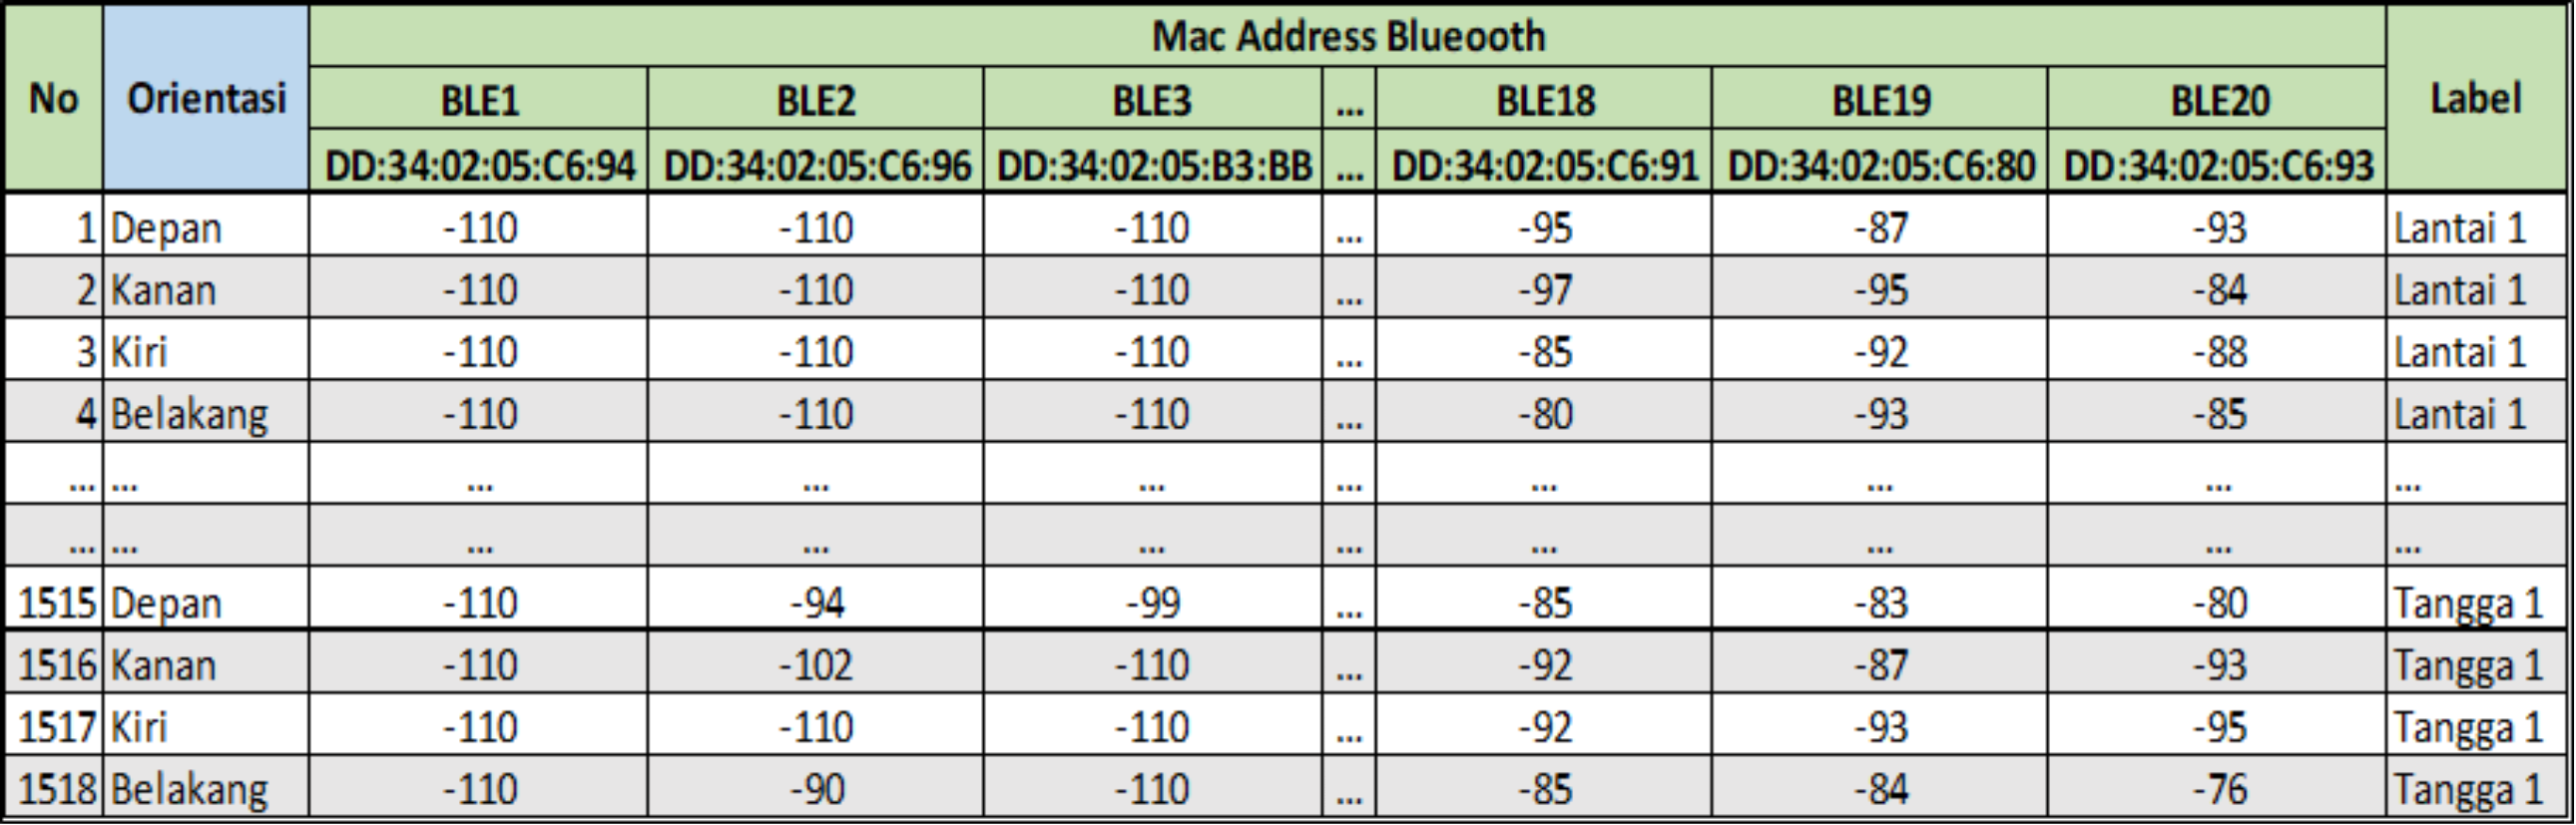
\includegraphics[width=25cm, height=7cm]{gambar/tes}
			      \label{fingerprinting}
		      \end{table}
	      \end{landscape}



	      \vspace{3cm}

	\item Pengumpulan Data Uji
	      \\
	      Pengumpulan data uji dilakukan setelah pengumpulan data \textit{training}. Data uji bertindak seolah-olah kelas label belum diketahui. Data uji tersebut akan dibandingkan dengan data \textit{training}, hasil tersebut akan diimplementasikan pada Aplikasi Penentuan Lokasi dan Estimasi Orang di dalam Gedung untuk memprediksi lokasi pengguna dengan metode klasifikasi \textit{Support Vector Machine} (SVM).

\end{enumerate}
%%%%%%%%%%%%%%%%%%%%%%%%%%%%%%%%%%%%%%%%%%%%%%%%%%%%%%%%%%%%%%%%%%%%%%%%%%%%%%%%%%%%%%%%%%%%%%%%%%%%%%%%%%%%%%%%%%%%%%%%%%%
%TESTING svm%
\subsection{Pengujian Akurasi dengan Metode Klasifikasi SVM}

\par Pengujian ini dilakukan dengan tujuan untuk mengetahui tingkat keberhasilan prediksi dengan menggunakan algoritma \textit{Support Vector Machine} (SVM) terhadap lokasi pengguna berdasarkan \textit{reference point} yang digunakan. Algoritma klasifikasi SVM pada penelitian ini dibuat dengan menggunakan kode python dengan tahapan sebagai berikut :

\begin{enumerate}[1.]
	\itemsep0em
	\item \textit{Import} library yang diperlukan
	      %   \begin{figure}[H]
	      %       \centering
	      %       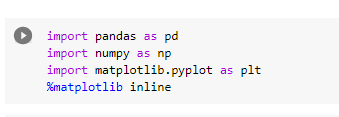
\includegraphics[width=14cm, height=3.5cm]{gambar/uji1}
	      %       \caption{\textit{Import} library yang diperlukan}
	      %       \label{uji1}
	      %   \end{figure}



	\item Memproses data atau membaca dataset dari hasil mapping
	      %   \begin{figure}[H]
	      %       \centering
	      %       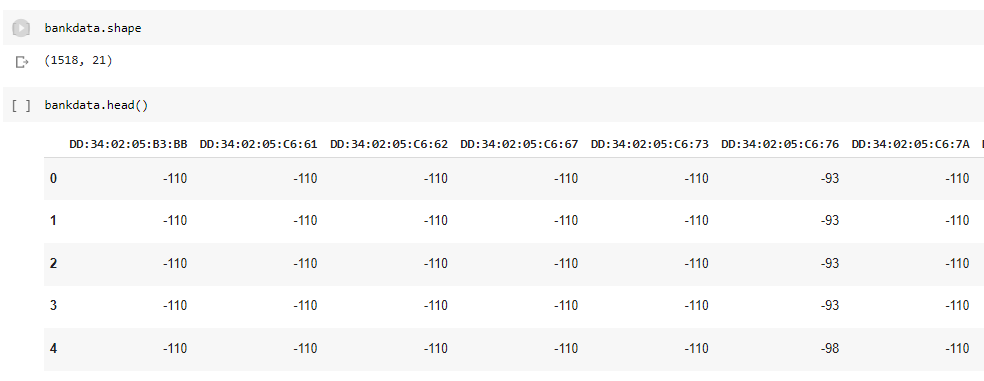
\includegraphics[width=14cm, height=6cm]{gambar/uji2}
	      %       \caption{Pemprosesan data atau membaca dataset dari hasil mapping}
	      %       \label{uji2}
	      %   \end{figure}

	\item Membagi data menjadi atribut dan label
	      %   \begin{figure}[H]
	      %       \centering
	      %       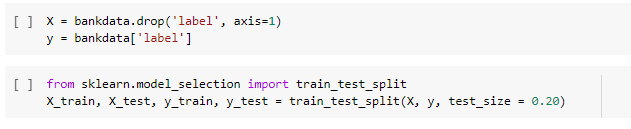
\includegraphics[width=14cm, height=4cm]{gambar/uji3}
	      %       \caption{Pembagian data menjadi atribut dan label}
	      %       \label{uji3}
	      %   \end{figure}

	\item Melatih Algoritma
	      %   \begin{figure}[H]
	      %       \centering
	      %       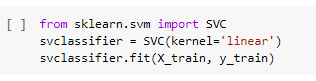
\includegraphics[width=13cm, height=4cm]{gambar/uji4}
	      %       \caption{Melatih Algoritme}
	      %       \label{uji4}
	      %   \end{figure}

	\item Menghasilkan model dan visualisasi hasil algoritma SVM.
	      \par Hasil tersebut adalah hasil akurasi dari klasifikasi algoritma SVM. Model dari algoritma SVM juga nantinya akan digunakan untuk memprediksi lokasi pengguna dalam penerapan aplikasi nantinya.

	\item Memprediksi
	      \par Proses ini akan memprediksi dengan memasukkan data \textit{testing} yang didapat dari proses pengambilan data uji menggunakan kode \textit{python}.
\end{enumerate}

\subsection{Pembuatan Model SVM}
Pada proses pembuatan model ini, dilakukan setelah proses pengujian akurasi dengan menggunakan algoritma klasifikasi \textit{Support Vector Machine} (SVM) dirasa sudah lebih akurat dengan dapat memprediksi semua klasifikasi yang diharapkan. Model dibuat dengan menggunakan bahasa kode python yang memanfaatkan library dari python yaitu \textit{pandas}, \textit{numpy}, dan \textit{matplotlib}. Setelah model berhasil dibuat maka model akan dimasukkan ke dalam \textit{web service flask}, dari \textit{web service flask} ini akan menghasilkan prediksi dari model dan akan dikirim ke aplikasi utama.


\subsection{Pembuatan Aplikasi Penentuan Lokasi dan Estimasi Orang dalam Gedung}
\begin{enumerate}


	\item Aplikasi Penentuan Lokasi dan Estimasi Jumlah Orang di dalam Gedung
	      \newline
	      Aplikasi yang dibangun menggunakan \textit{react native} ini adalah aplikasi berbasis Android yang berguna untuk mempermudah pengguna dan rekan tim penelitian untuk melakukan proses
	      pencarian lokasi dan estimasi jumlah orang yang berada di dalam gedung Blok A Fakultas Matematika dan Ilmu Pengetahuan Alam Universitas Syiah Kuala, yang dikembangkan dengan konsep \textit{Indoor Localization System} dan \textit{Crowdsourcing}. Aplikasi ini bekerja apabila perangkat smartphone sudah mendukung Bluetooth 4.0, dikarenakan aplikasi ini menangkap kekuatan sinyal atau nilai RSSI dari \textit{Beacon} yang terintegrasi BLE di dalamnya. Kekuatan sinyal yang ditangkap akan dilakukan perhitungan menggunakan metode klasifikasi \textit{Support Vector Machine} (SVM), output dari perhitungan tersebut adalah prediksi lokasi pengguna yang akan dikirim ke web services flask secara background process. Adapun fitur-fitur yang tersedia adalah sebagai berikut:.

	      \begin {itemize}
	      \itemsep0em
	\item Memprediksi Lokasi Pengguna saat berada di dalam gedung\newline

	\item Menampilkan Estimasi Jumlah Orang yang Berada di dalam Gedung Blok A Fakultas Matematika dan Ilmu Pengetahuan Alam Universitas Syiah Kuala

	      \end{itemize}
\end{enumerate}
%%%%%%%%%%%%%%%%%%%%%%%%%%%%%%%%%%%%%%%%%%%%%%%%%%%%%%%%%%%%%%%%%%%%%%%%%%%%%%%%%%%%%%%%%%%%%%%%%%%%%%%%%%%%%%%%%%%%%%%%%%%%%%%
\subsection{Pengujian Fungsionalitas dengan Metode Black Box}
\par Pengujian \textit{Black Box} berfokus pada spesifikasi fungsionalitas dari sistem yang telah dibuat dengan mengeksekusi dan menjalankan sistem tersebut apakah sesuai dengan alur bisnis yang diinginkan. Pengujian ini melihat fungsi yang tidak sesuai pada sistem, kesalahan-kesalahan sistem dalam mengerjakan suatu perintah, dan kesalahan-kesalahan pada struktur data dan akses basis data.

\subsection{Pengujian Usability dengan Metode UMUX}
\par Usability Testing dilakukan agar bisa mengevaluasi suatu produk atau jasa yang dihasilkan dengan cara menguji kepada calon pengguna dengan menggunakan metode UMUX. UMUX terdiri dari 4 pertanyaan dengan menggunakan skala likert 1-7. Skala likert adalah sebuah metode skala yang bersifat bipolar yang akan mengukur tanggapan positif dan negatif terhadap sebuah pertanyaan. Berikut daftar pertanyaan-pertanyaan metode UMUX dapat dilihat pada \ref{tabel-pertanyaan-umux}.
%TABEL PERTANYAAN umux%
\begin{table}[H]
	\center
	\caption{Daftar Pertanyaan Metode UMUX \citep{Finstad2010}}
	\label{tabel-pertanyaan-umux}
	\begin{tabular}{|l|l|l|}
		\hline
		\rowcolor[HTML]{656565}
		{\color[HTML]{343434} No.} & Pertanyaan                                                                                                                 & Skor \\ \hline
		1                          & Aplikasi ini sesuai dengan kebutuhan saya                                                                                  & 1-7  \\
		\hline
		2                          & Saya memiliki pengalaman buruk dalam menggunakan aplikasi ini                                                              & 1-7  \\
		\hline
		3                          & Aplikasi ini mudah digunakan                                                                                               & 1-7  \\
		\hline
		4                          & \begin{tabular}[c]{@{}l@{}}Saya harus mengabiskan banyak waktu \\ untuk menggunakan aplikasi ini dengan benar\end{tabular} & 1-7  \\ \hline
	\end{tabular}
\end{table}

% \par Rumus untuk menghitung skor akhir metode SUS \citep{Brooke1996}, dapat dilihat dari persamaan berikut.
% \begin{equation}
% 	skorSUS = (\sum_{9}^{i} (Ri - 1) + \sum_{10}^{j} (5 - Rj)) * 2,5
% \end{equation}
% \newline
% Keterangan:\newline
% $R$ = daftar pertanyaan pada metode SUS. \newline
% $i$ = angka ganjil 1, 3, 5, 7, dan 9. \newline
% $j$ = angka genap 2, 4, 6, 8, dan 10.
% \newline

\par Tingkat nilai skala pengujian menentukan apakah sistem tersebut layak digunakan, bermanfaat, diterima oleh \textit{user} dan bertahan lama penggunaannya. Sebuah sistem dengan nilai pengujian yang tinggi membuat sistem tersebut menjadi populer dalam waktu yang lama dan penggunaannya yang luas, karena banyak individu akan merasakan manfaat dari kehadiran sistem tersebut. Sedangkan sistem dengan nilai pengujian yang rendah, seringkali diabaikan oleh pengguna walaupun dibuat berdasarkan kebutuhan dan menghasilkan sumber daya yang banyak. Berdasarkan dari skor akhir SUS tersebut, dapat diketahui bahwa seberapa tinggi tingkat \textit{usability} perancangan sistem yang dikembangkan. Tabel \ref{tabelsus} menunjukkan nilai interpretasi yang digunakan.

\begin{table}[H]
	\center
	\caption{Interpretasi skor SUS \citep{Bangoor2009}.}
	\label{tabelsus}
	\begin{tabular}{|c|c|lll}
		\cline{1-2}
		\textbf{Skor SUS} & \textbf{Interprestasi} &  &  & \\ \cline{1-2}
		\textless{}50     & Tidak Dapat Diterima   &  &  & \\ \cline{1-2}
		50-70             & Marginal               &  &  & \\ \cline{1-2}
		\textgreater{}70  & Dapat Diterima         &  &  & \\ \cline{1-2}
	\end{tabular}
\end{table}

%%%%%%%%%%%%%%%%%%%%%%%%%%%%%%%%%%%%%%%%%%%%%%%%%%%%%%%%%%%%%%%%%%%%%%%%%%%%%%%%%%%%%%%%%%%%%%%%%%%%%%%%%%%%%%%%
\subsection{Analisis Keakuratan}
Penelitian ini memiliki dua analisis keakuratan dalam penentuan lokasi pengguna. Analisis keakuratannya adalah sebagai berikut:
\begin{enumerate}[1.]
	\item Membandingkan tingkat keakuratan klasifikasi antara \textit{reference point} urut dan \textit{reference point} acak.
	\item Membandingkan tingkat keakuratan dalam memprediksi lokasi pengguna menggunakan jumlah \textit{Beacon} yang berbeda, yaitu dengan jumlah 3 \textit{Beacon} dan 6 \textit{Beacon}.
\end{enumerate}


  %-------------------------------------------------------------------------------
%                            BAB IV
%               		HASIL DAN PEMBAHASAN
%-------------------------------------------------------------------------------
\fancyhf{} 
\fancyfoot[C]{\thepage}
\chapter{HASIL DAN PEMBAHASAN}
	\section{\uppercase{ANALISIS KEBUTUHAN}}
	
	Hasil dari analisis kebutuhan yang telah dilakukan adalah mendapatkan kelompok pengguna yang akan terlibat dalam penelitian dan \textit{use case diagram} untuk masing-masing pengguna. Berikut hasil analisis kebutuhan dari sistem yang dibangun.
	
	\subsection{Kelompok Pengguna}
	Kelompok pengguna dari aplikasi ini telah dapat diidentifikasikan pada tahap analisis kebutuhan pada sistem. terdapat 2 kelompok pengguna yang menggunakan aplikasi ini:
		 \begin{enumerate}[1.]
		 	\item Peneliti
		 		\newline Pengguna yang menggunakan Aplikasi Mapping berbasis Android untuk melakukan pemetaan kekuatan sinyal atau nilai RSSI dari Beacon. 
		 	\item Dosen
		 		\newline Pengguna yang menggunakan Aplikasi Kehadiran Dosen berbasis Android untuk melakukan pencatatan kehadiran sebagai pengajar suatu mata kuliah.
		 	\item Mahasiswa
		 		\newline Pengguna yang menggunakan Aplikasi Kehadiran berbasis Android untuk melakukan pencatatan kehadiran sebagai peserta belajar suatu mata kuliah.
		 	\item Admin
		 		\newline Pengguna yang menggunakan Aplikasi Rekap Kehadiran Dosen dan Mahasiswa berbasis web untuk memantau dan merekap kehadiran dosen dan mahasiswa pada suatu mata kuliah.
		 	\end{enumerate}
	
	\subsection{Use Case Diagram}
	\textit{Use case} merupakan pemodelan untuk mendeskripsikan sebuah interaksi antara satu atau lebih aktor dengan sistem yang dibuat. Secara kasar, \textit{use case} digunakan untuk mengetahui fungsi apa saja yang ada di dalam sebuah sistem dan siapa saja yang berhak menggunakan fungsi-fungsi itu \citep{Rosa2015}. \textit{Use Case Diagram} dari sistem yang telah dibangun dapat dilihat pada Gambar \ref{usecasemapping}, Gambar \ref{usecasedosen}, Gambar \ref{usecasemahasiswa} dan Gambar \ref{usecaseadmin}.
	
	\begin{figure}[H]
		\center
		\shadowbox
		{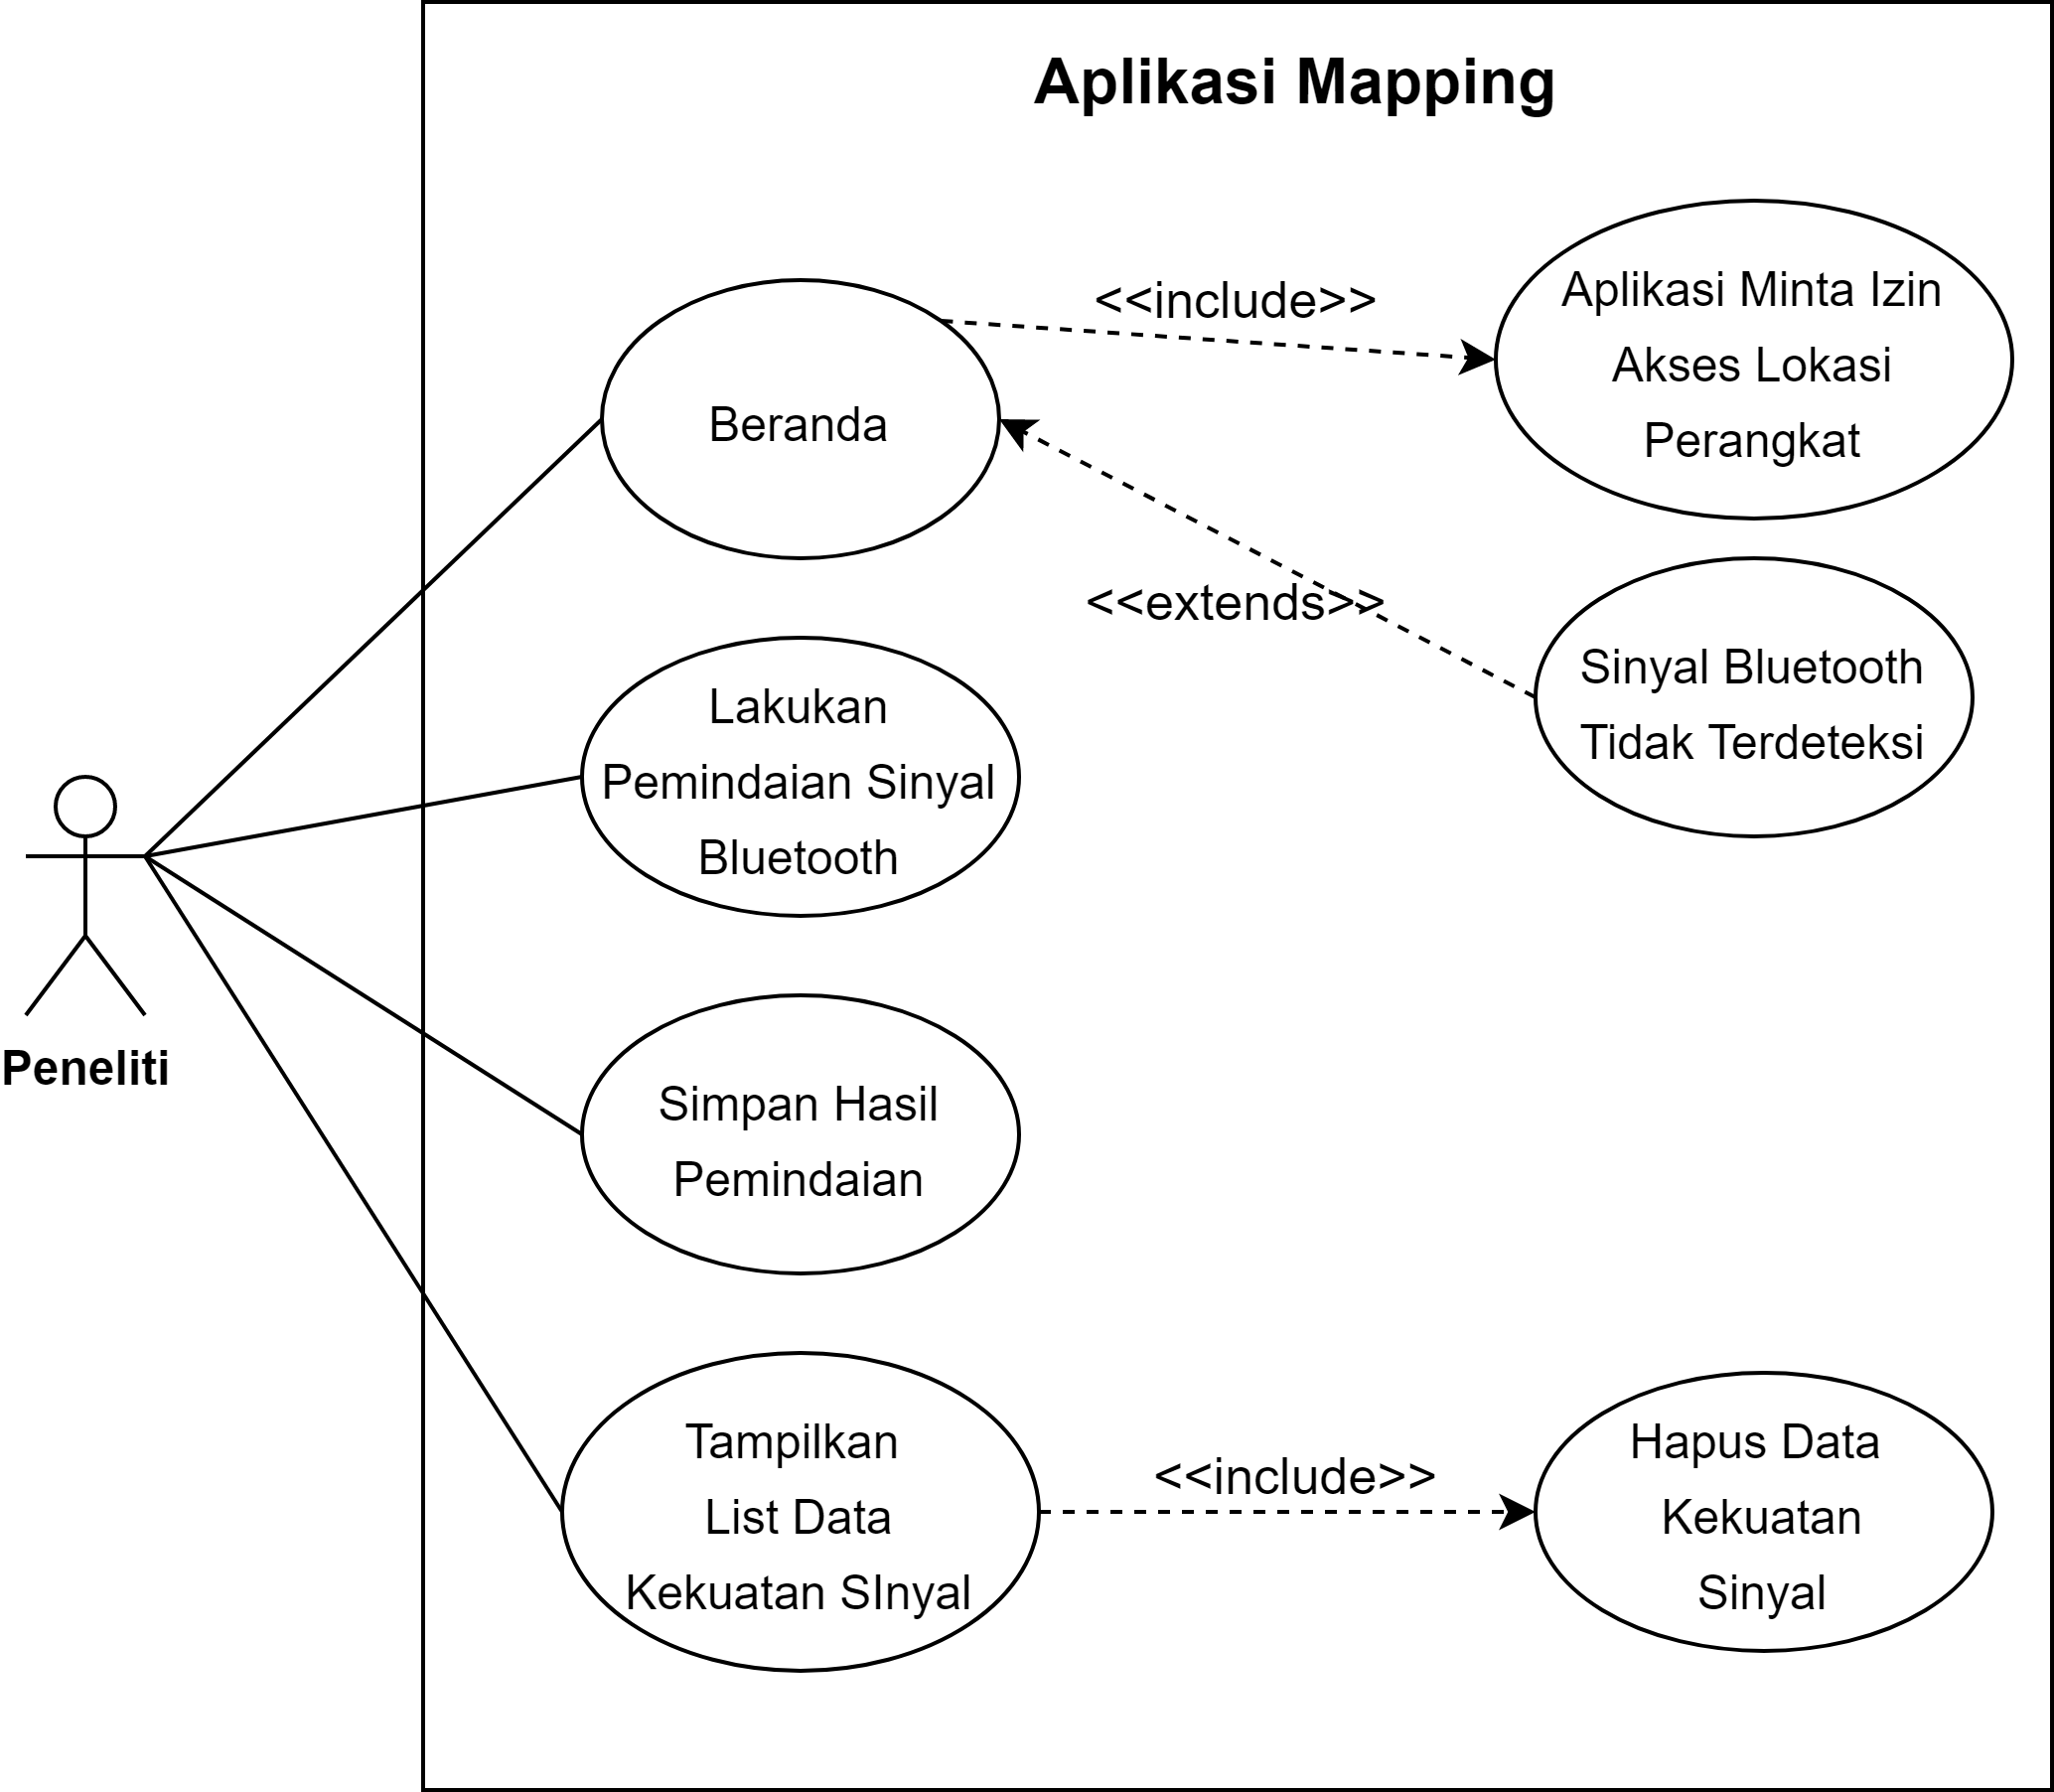
\includegraphics [width=7.5cm, height=7cm]{gambar/model/use-case-mapping}}
		\caption{\textit{Use Case Diagram} Aplikasi Mapping.}
		\label{usecasemapping}
	\end{figure}
	
\par Gambar \ref{usecasemapping} diatas menjelaskan aktivitas yang dapat dilakukan oleh peneliti saat menggunakan aplikasi. Ketika peneliti membuka aplikasi, muncul halaman beranda. Selanjutnya, peneliti diminta untuk mengizinkan aplikasi mengakses lokasi pada perangkat. Kemudian, peneliti dapat melakukan pemindaian kekuatan sinyal setelah menghidupkan Bluetooth pada perangkat. Setelah itu, hasil dari pemindaian kekuatan sinyal tersebut disimpan, lalu dapat ditampilkan pada sebuah halaman. Pengguna juga dapat menghapus data-data kekuatan sinyal sesuai keinginan.
\fancyhf{} 
\fancyfoot[R]{\thepage}

\begin{figure}[H] 
		\center
		\shadowbox
		{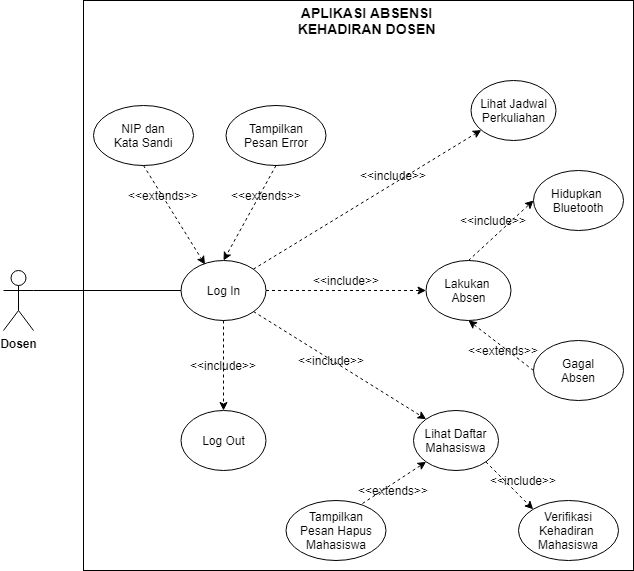
\includegraphics [width=10cm, height=9cm]{gambar/model/use-case-dosen}}
		\caption{\textit{Use Case Diagram} Aplikasi Kehadiran Dosen.}
		\label{usecasedosen}
	\end{figure}

\par Gambar \ref{usecasedosen} menjelaskan aktivitas yang dapat dilakukan oleh dosen saat menggunakan aplikasi. Aktivitas pertama yang dilakukan adalah melakukan \textit{log in} ke aplikasi dengan memasukkan Nomor Induk Pegawai (NIP) dan kata sandi. Setelah melakukan \textit{log in}, dosen dapat menikmati fitur-fitur yang tersedia seperti melihat jadwal perkuliahan, memulai proses kehadiran dengan syarat keadaan Bluetooth pada perangkat dalam keadaan hidup dan melihat daftar mahasiswa yang mengambil suatu mata kuliah. Aktivitas yang terakhir adalah \textit{log out}, yaitu aktivitas yang berfungsi untuk keluar dari aplikasi. Apabila dosen telah melakukan \textit{log out}, maka dosen harus melakukan \textit{log in} kembali ke aplikasi.
	
	\begin{figure}[H] 
		\center
		\shadowbox
		{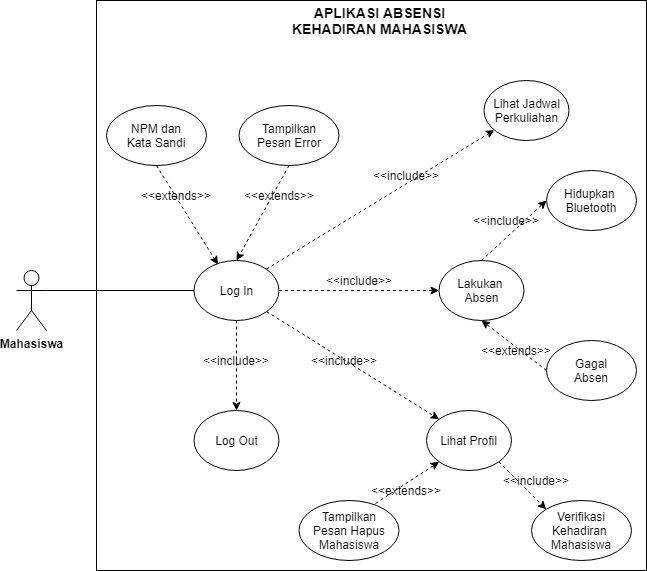
\includegraphics [width=10cm, height=9.5cm]{gambar/model/use-case-mahasiswa}}
		\caption{\textit{Use Case Diagram} Aplikasi Kehadiran Mahasiswa.}
		\label{usecasemahasiswa}
	\end{figure}
	
\par Gambar \ref{usecasemahasiswa} diatas menjelaskan aktivitas yang dapat dilakukan oleh mahasiswa saat menggunakan aplikasi. Aktivitas pertama yang dilakukan adalah melakukan \textit{log in} ke aplikasi dengan memasukkan Nomor Pokok Mahasiswa (NPM) dan kata sandi. Setelah melakukan \textit{log in}, mahasiswa dapat menikmati fitur-fitur yang tersedia seperti melihat jadwal perkuliahan, memulai proses kehadiran dengan syarat keadaan Bluetooth pada perangkat dalam keadaan hidup dan melihat profil data diri. Aktivitas yang terakhir adalah \textit{log out}, yaitu aktivitas yang berfungsi untuk keluar dari aplikasi. Apabila mahasiswa telah melakukan \textit{log out}, maka mahasiswa harus melakukan \textit{log in} kembali ke aplikasi.

	\begin{figure}[H] 
		\center
		\shadowbox
		{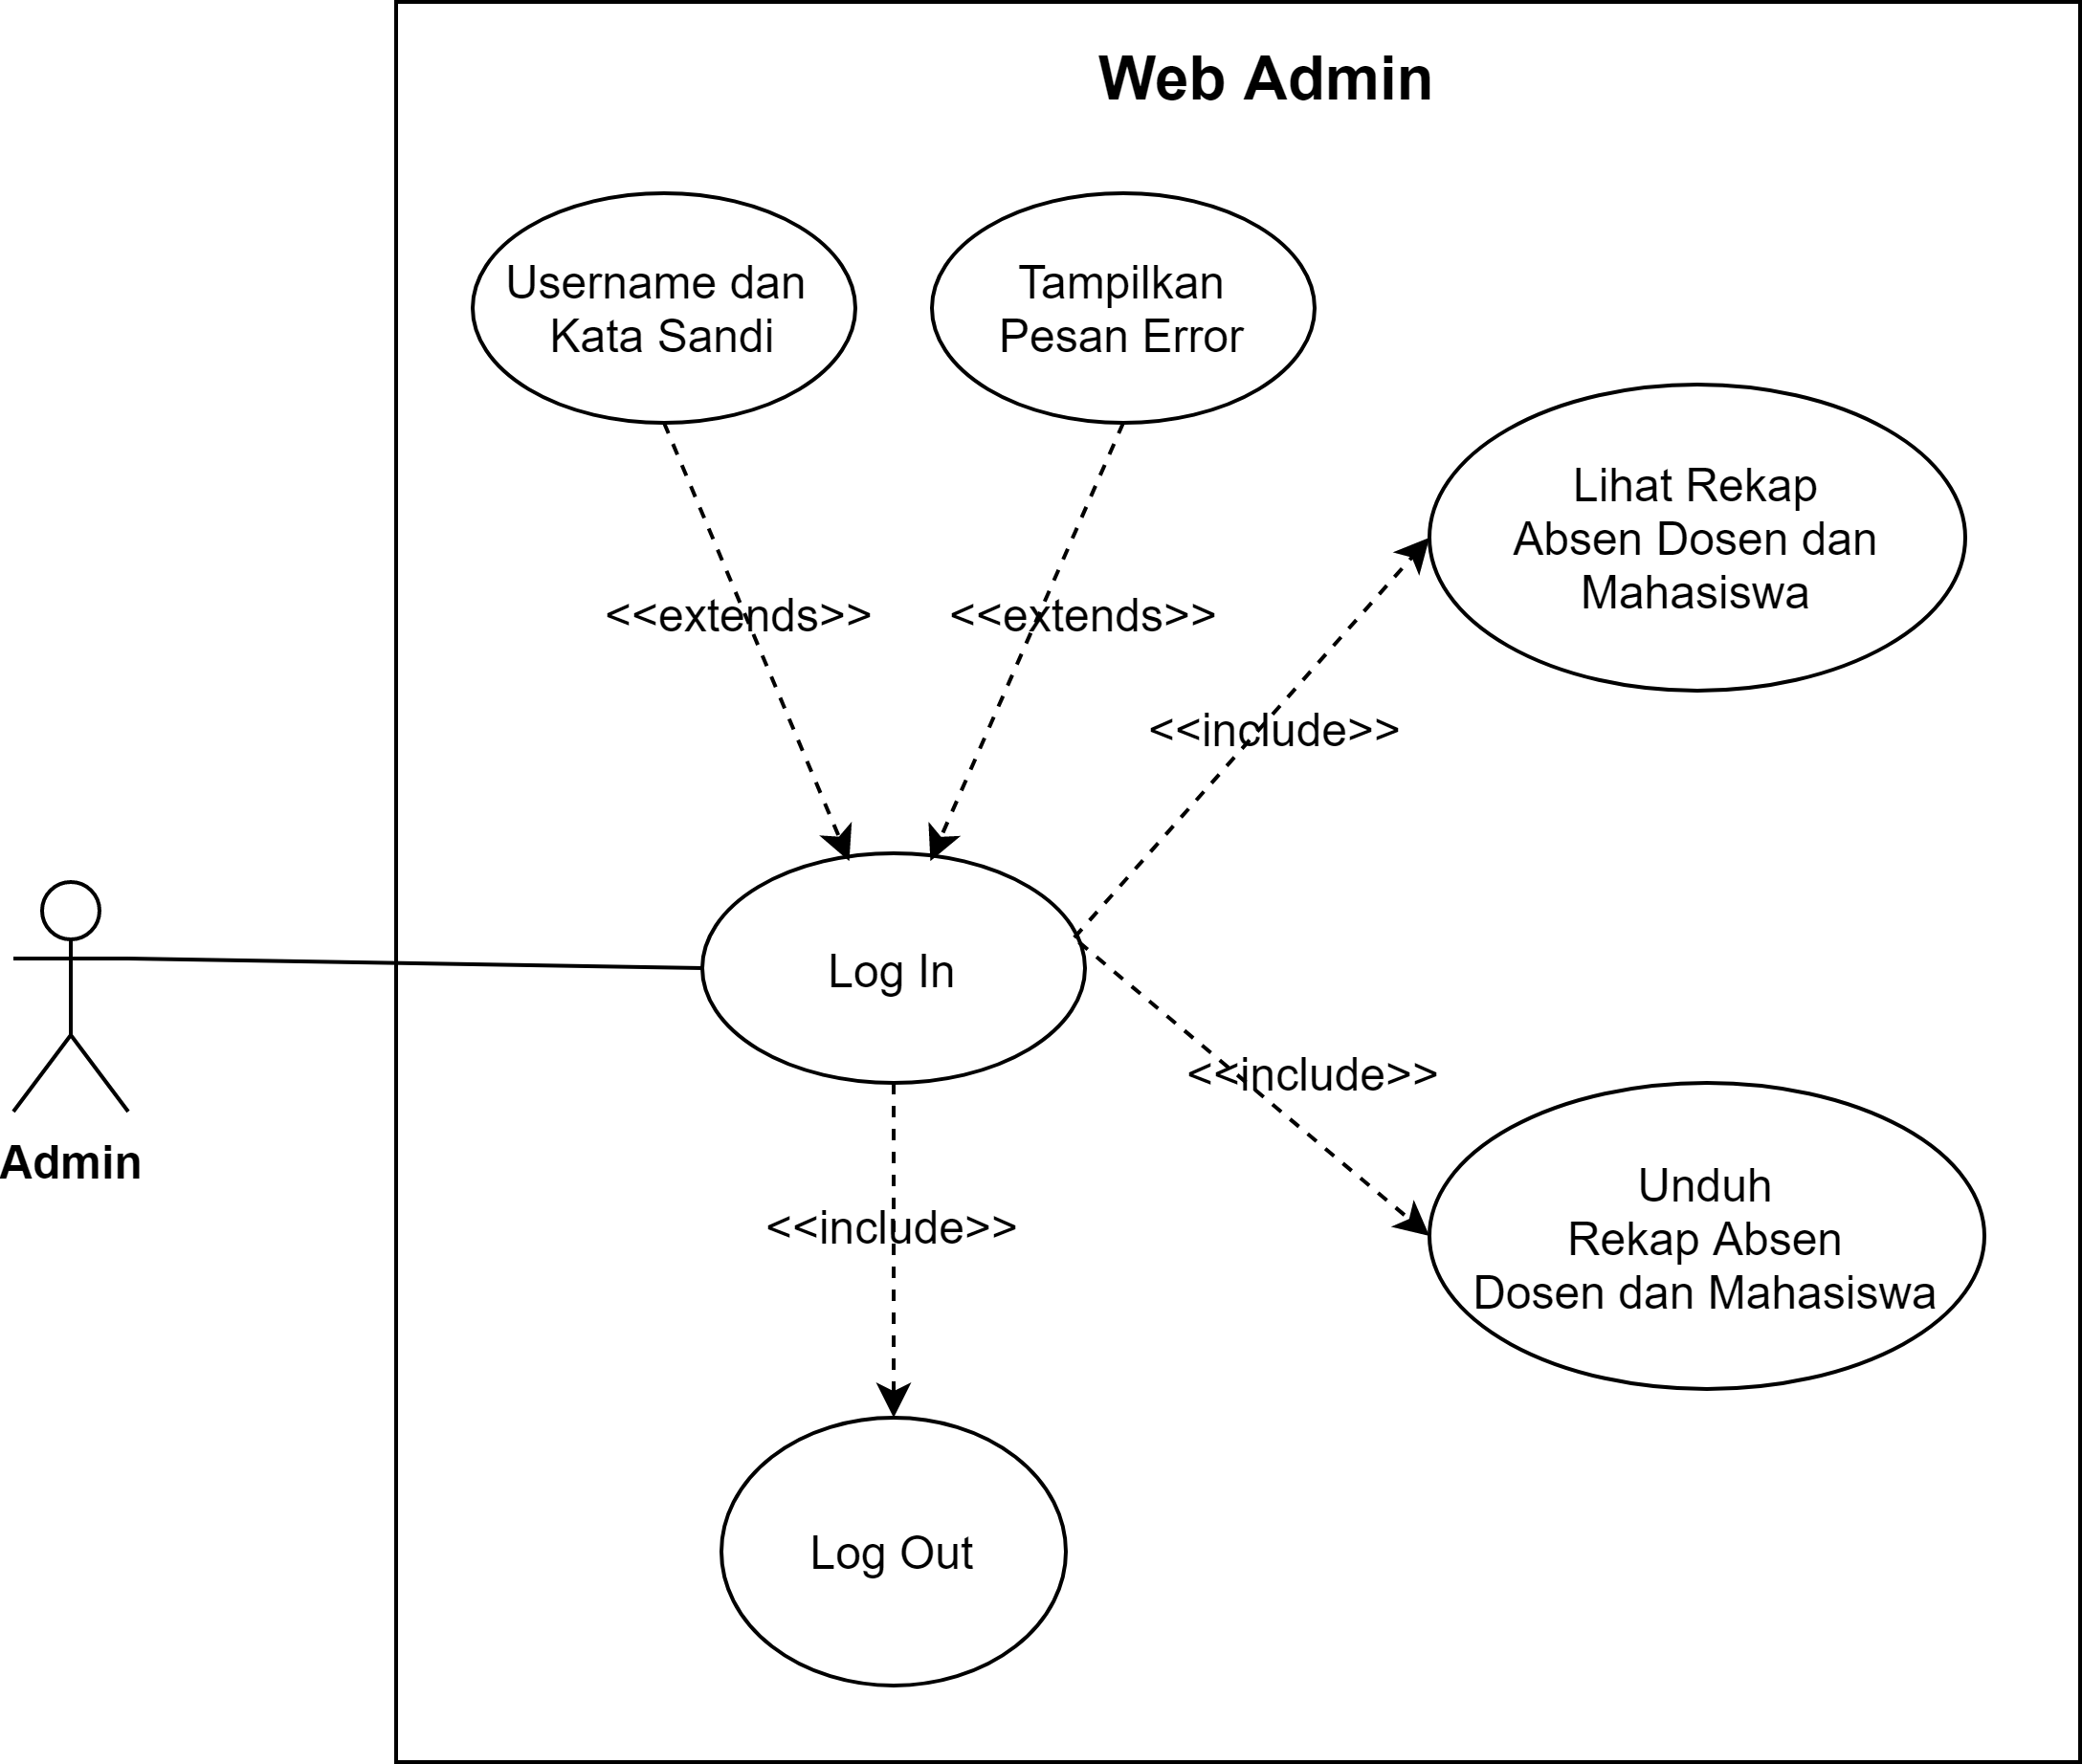
\includegraphics [width=9cm, height=8cm]{gambar/model/use-case-admin}}
		\caption{\textit{Use Case Diagram} Aplikasi Rekap Kehadiran Dosen dan Mahasiswa (Web-Based).}
		\label{usecaseadmin}
	\end{figure}
	
\par Gambar \ref{usecaseadmin} diatas menjelaskan aktivitas yang dapat dilakukan oleh admin saat menggunakan aplikasi. Aktivitas pertama yang dilakukan adalah melakukan \textit{log in} ke aplikasi dengan memasukkan \textit{username} dan kata sandi. Setelah melakukan \textit{log in}, admin dapat melihat daftar kehadiran dosen dan mahasiswa pada mata kuliah tertentu. Selain itu, admin juga dapat mengunduh data-data kehadiran tersebut.
	


	\section{\uppercase{PERANCANGAN DAN PEMBUATAN SISTEM}}
	
	\subsection{Perancangan Sistem}
	\par Perancangan sistem merupakan tahapan proses desain dari sistem perangkat lunak yang dibuat. Proses ini terdiri dari dua tahap yaitu perancangan konfigurasi eksekusi sistem dalam bentuk \textit{deployment diagram} dan perancangan tampilan antar muka (\textit{interface}).
	
   	%Tahap pertama adalah merancang \textit{class diagram} yang bertujuan untuk menggambarkan struktur sistem dari segi pendefinisian dari kelas-kelas yang dibuat untuk membangun sistem. Kelas-kelas yang ada pada struktur sistem harus dapat melakukan fungsi-fungsi sesuai dengan kebutuhan sistem. %Berikut rancangan \textit{class diagram} dari sistem yang telah dibangun dapat dilihat pada Gambar:
   			%\begin{enumerate}
     			%\item \textit{Class Diagram} Aplikasi Mapping
					%\vspace{-0.2cm}
					%\begin{figure}[H]
						%\center
						%\includegraphics [width = 14cm]{gambar/model/class-diagram}
						%\caption{Diagram Kelas Model Basis Data }
					%\label{class}
					%\end{figure}
									
     			%\item \textit{Class Diagram} Aplikasi Kehadiran Dosen
     			%\item \textit{Class Diagram} Aplikasi Kehadiran Mahasiswa
   			%\end{enumerate}
 	%Tahap kedua adalah merancang \textit{component diagram}, dimana \textit{component diagram} dibuat untuk menunjukkan organisasi dan ketergantungan diantara kumpulan komponen dalam sebuah sistem, serta pemodelan bagaimana sistem beradaptasi dengan sistem lain. Berikut rancangan \textit{component diagram} dari sistem yang telah dibangun dapat dilihat pada Gambar \ref{componentmapping} dan Gambar \ref{componentabsensi}.
 			%\begin{enumerate}
     			%\item \textit{Component Diagram} Aplikasi Mapping
					%\vspace{-0.2cm}
					%\begin{figure}[H]
						%\center
						%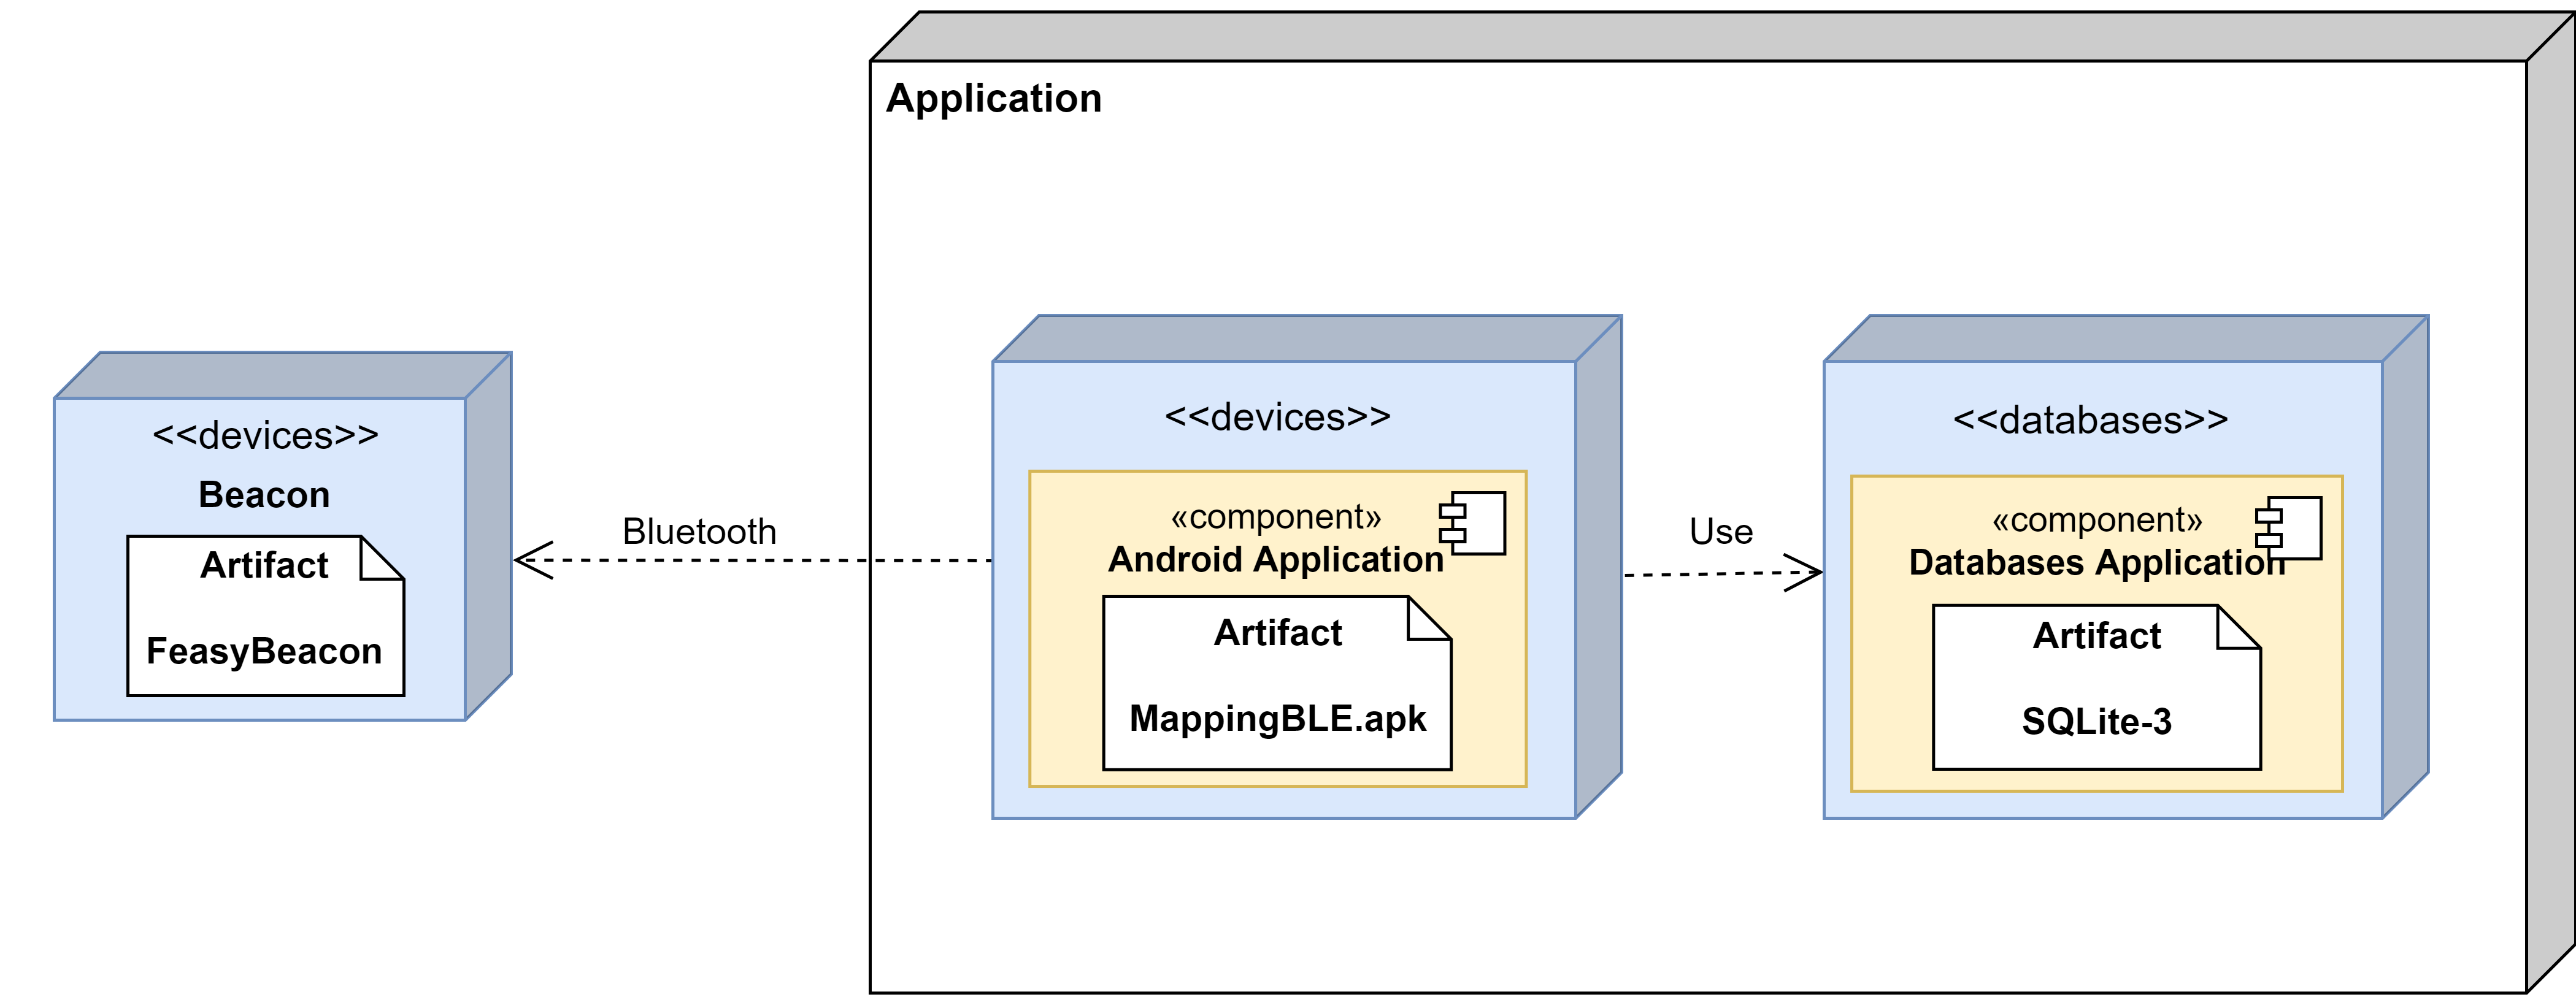
\includegraphics [width = 13cm, height= 5cm]{gambar/model/component-diagram-mapping}
						%\caption{Diagram Component Aplikasi Mapping}
					%\label{componentmapping}
					%\end{figure}
									
     			%\item \textit{Component Diagram} Aplikasi Kehadiran Dosen dan Aplikasi Kehadiran Mahasiswa
     				%\vspace{-0.2cm}
					%\begin{figure}[H]
						%\center
						%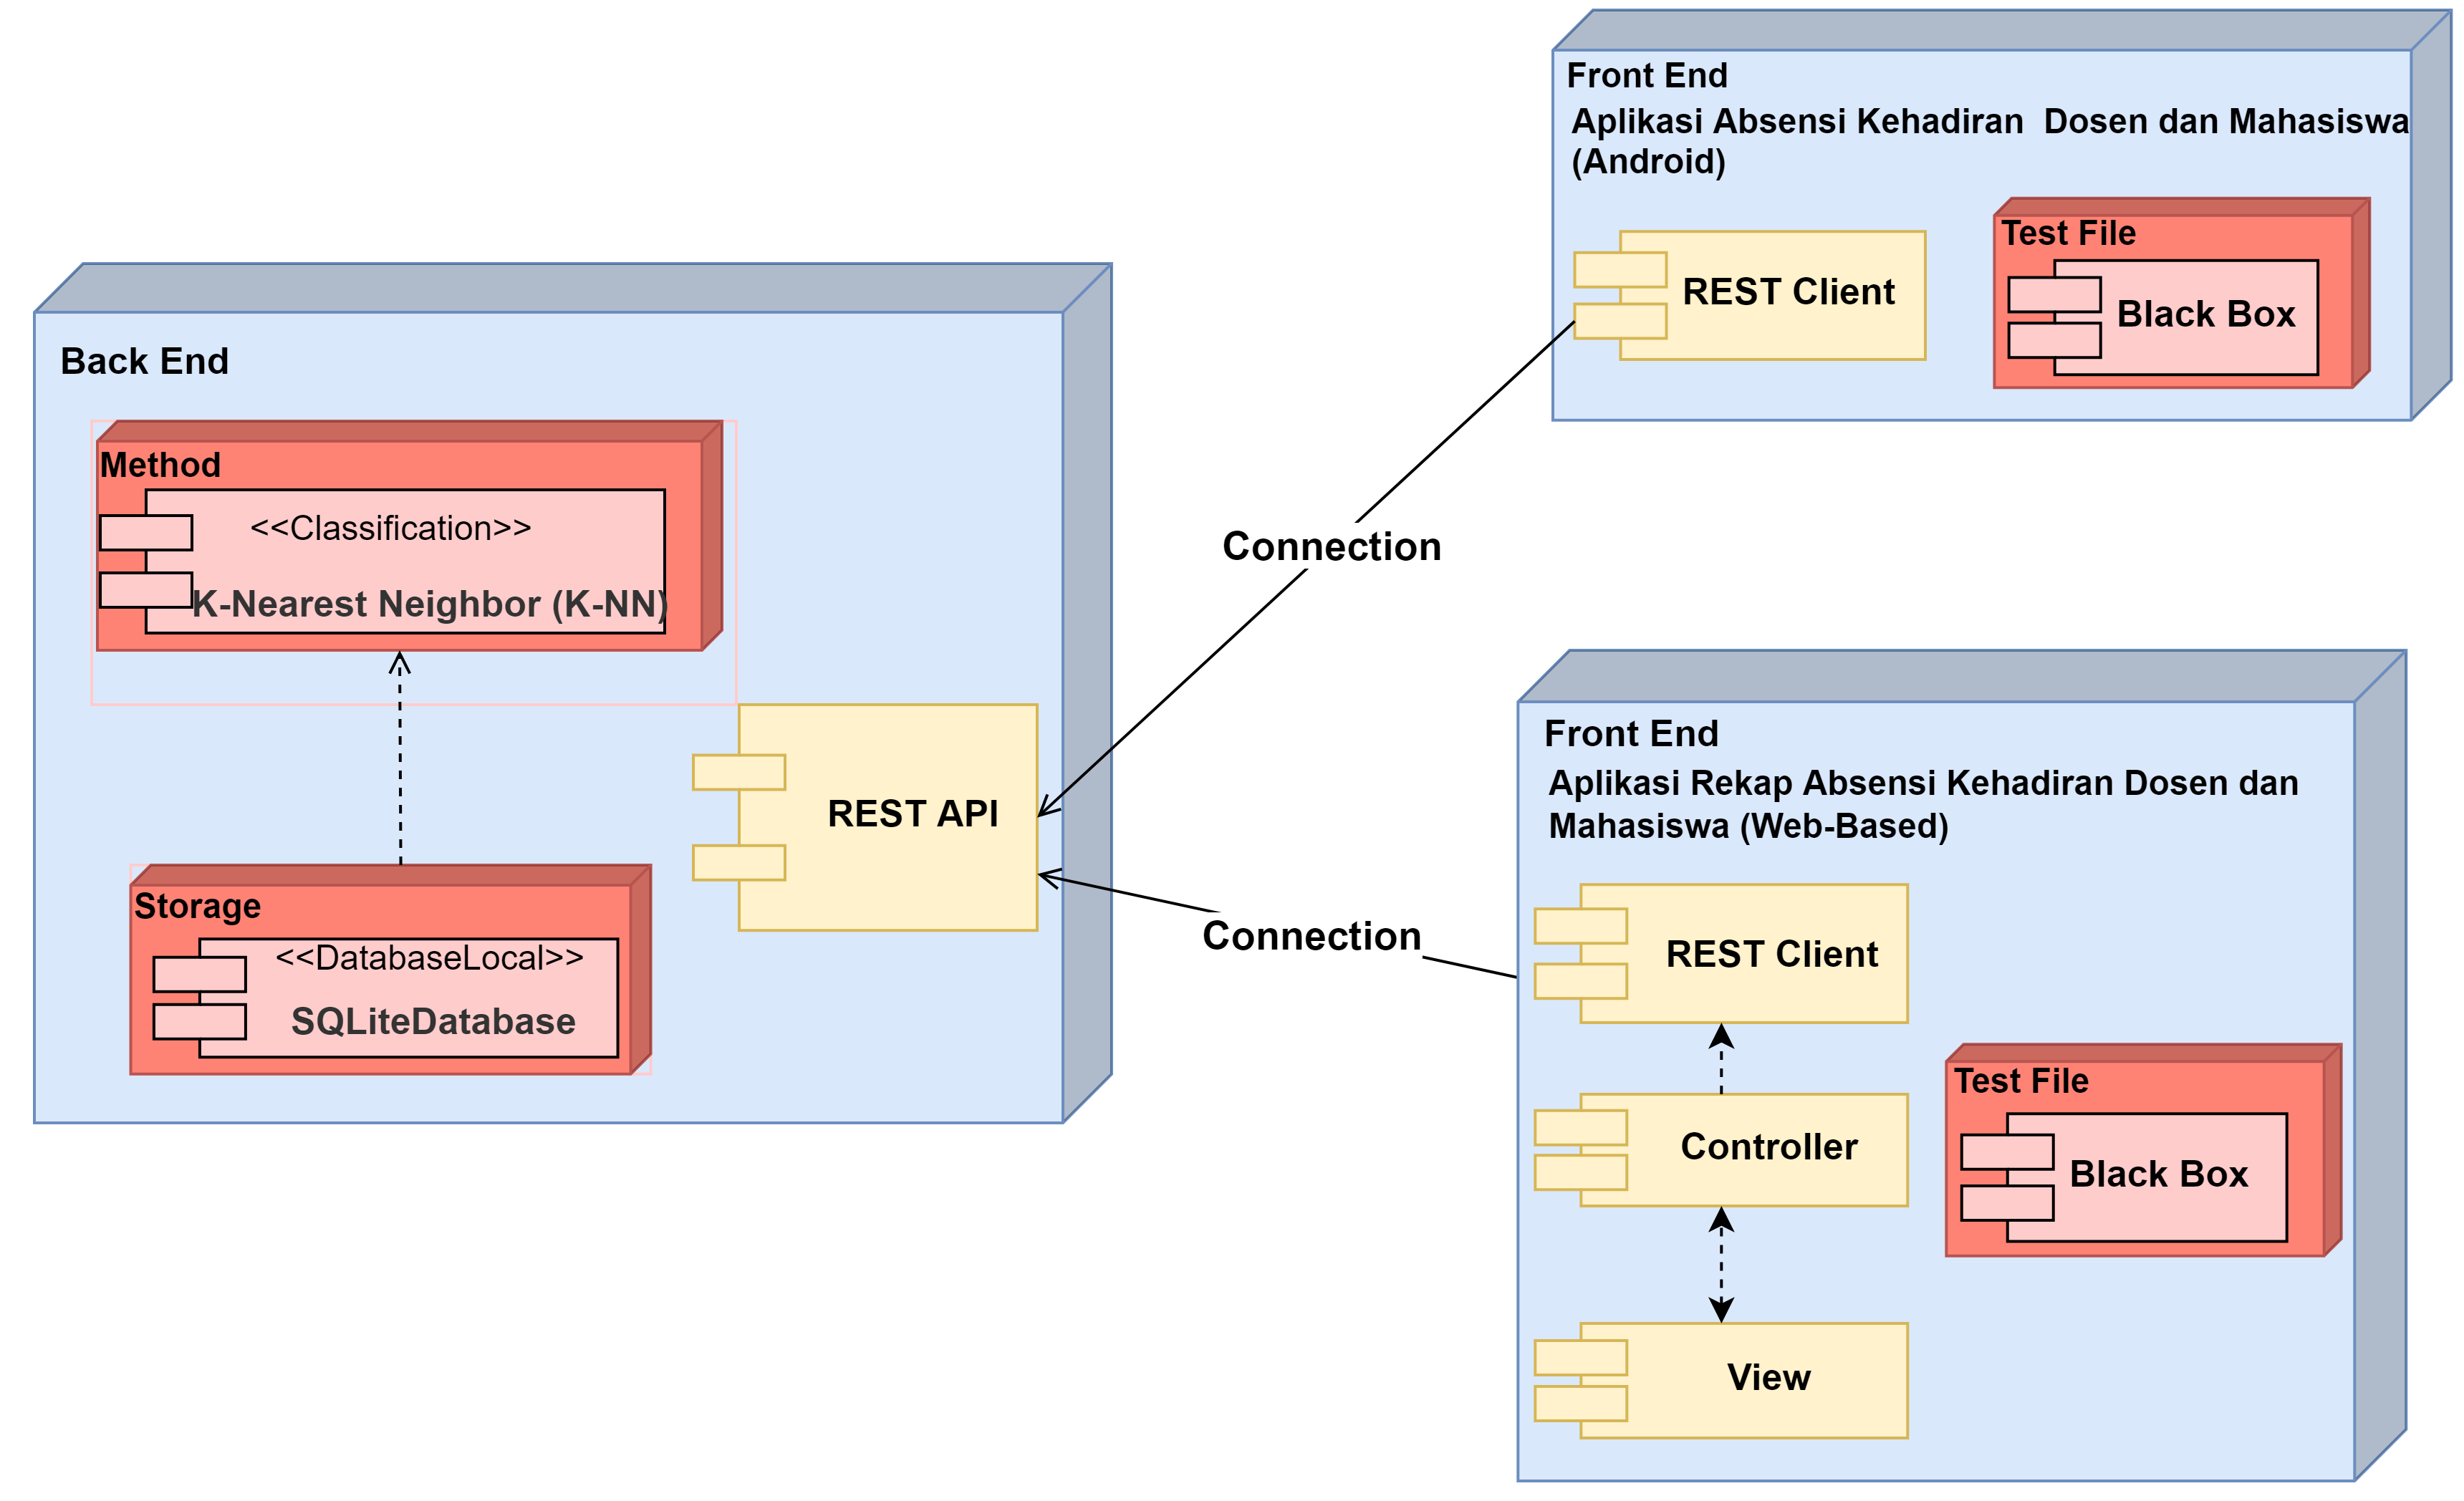
\includegraphics [width = 13.5cm, height= 9cm]{gambar/model/component-diagram-absensi}
						%\caption{Diagram Component Aplikasi Kehadiran Dosen dan Mahasiswa}
					%\label{componentabsensi}
					%\end{figure}
   			%\end{enumerate}
   	Tahap pertama adalah merancang \textit{deployment diagram}, dimana \textit{deployment diagram} adalah diagram yang menjelaskan bagaimana sistem bekerja dan digunakan oleh pengguna. Berikut rancangan \textit{deployment diagram} dari sistem yang telah dibangun dapat dilihat pada Gambar \ref{deployment-diagram}.
   		
 			%\begin{enumerate}
     			%\item \textit{Deployment Diagram} Aplikasi Mapping
					\vspace{-0.2cm}
				 \begin{landscape}
					\begin{figure}[H]
						\center
						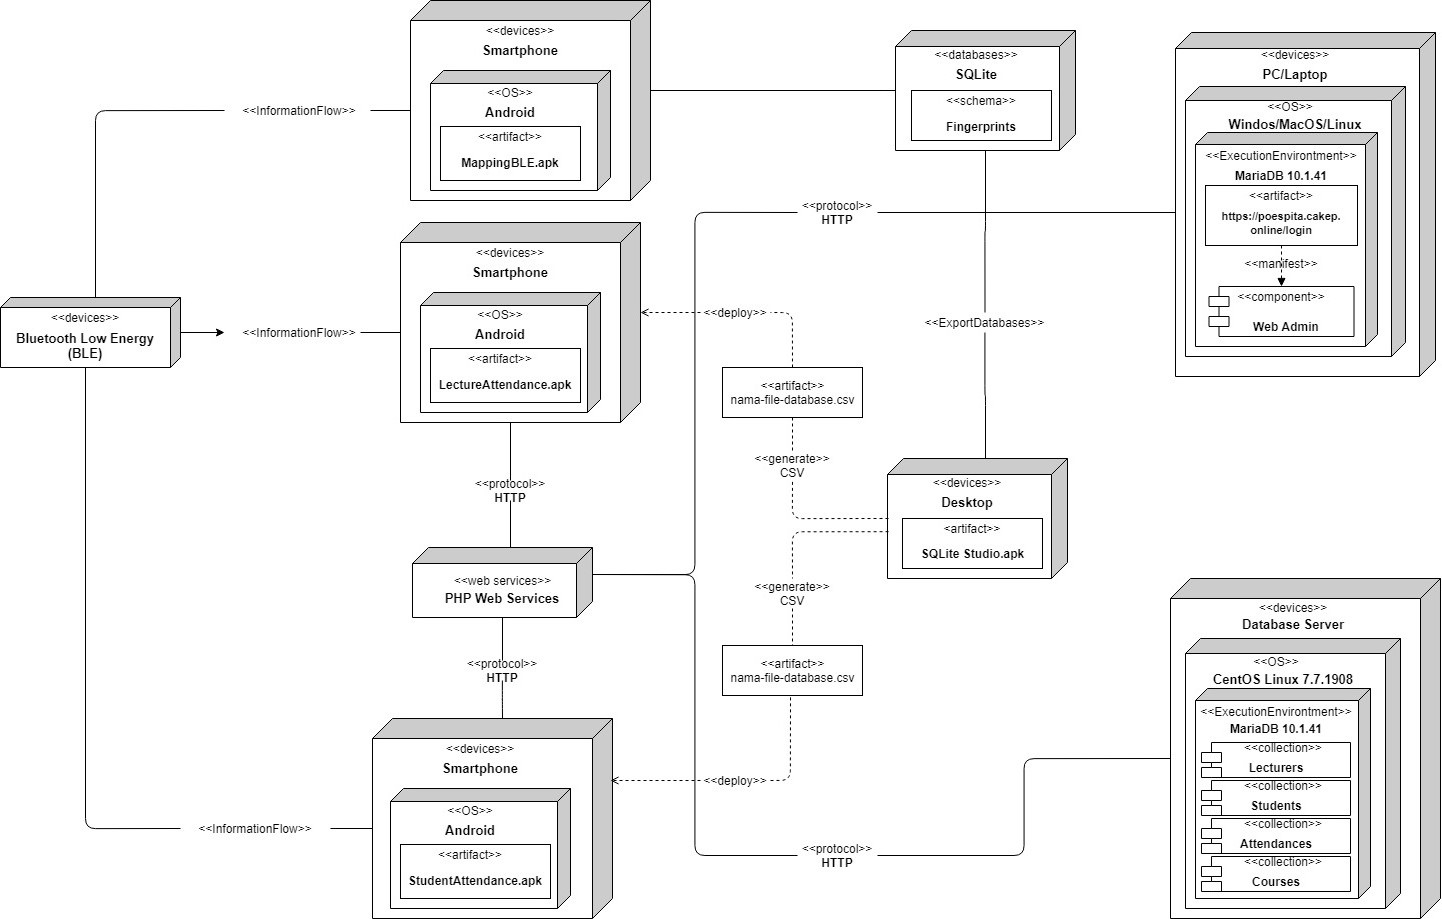
\includegraphics [width = 22.5cm, height=12cm]{gambar/model/deployment-diagram}
						\caption{Diagram \textit{Deployment}}
					\label{deployment-diagram}
					\end{figure}
				  \end{landscape}
									
     			%\item \textit{Deployment Diagram} Aplikasi Kehadiran Dosen dan Aplikasi Kehadiran Mahasiswa
     				%\vspace{-0.2cm}
					%\begin{figure}[H]
						%\center
						%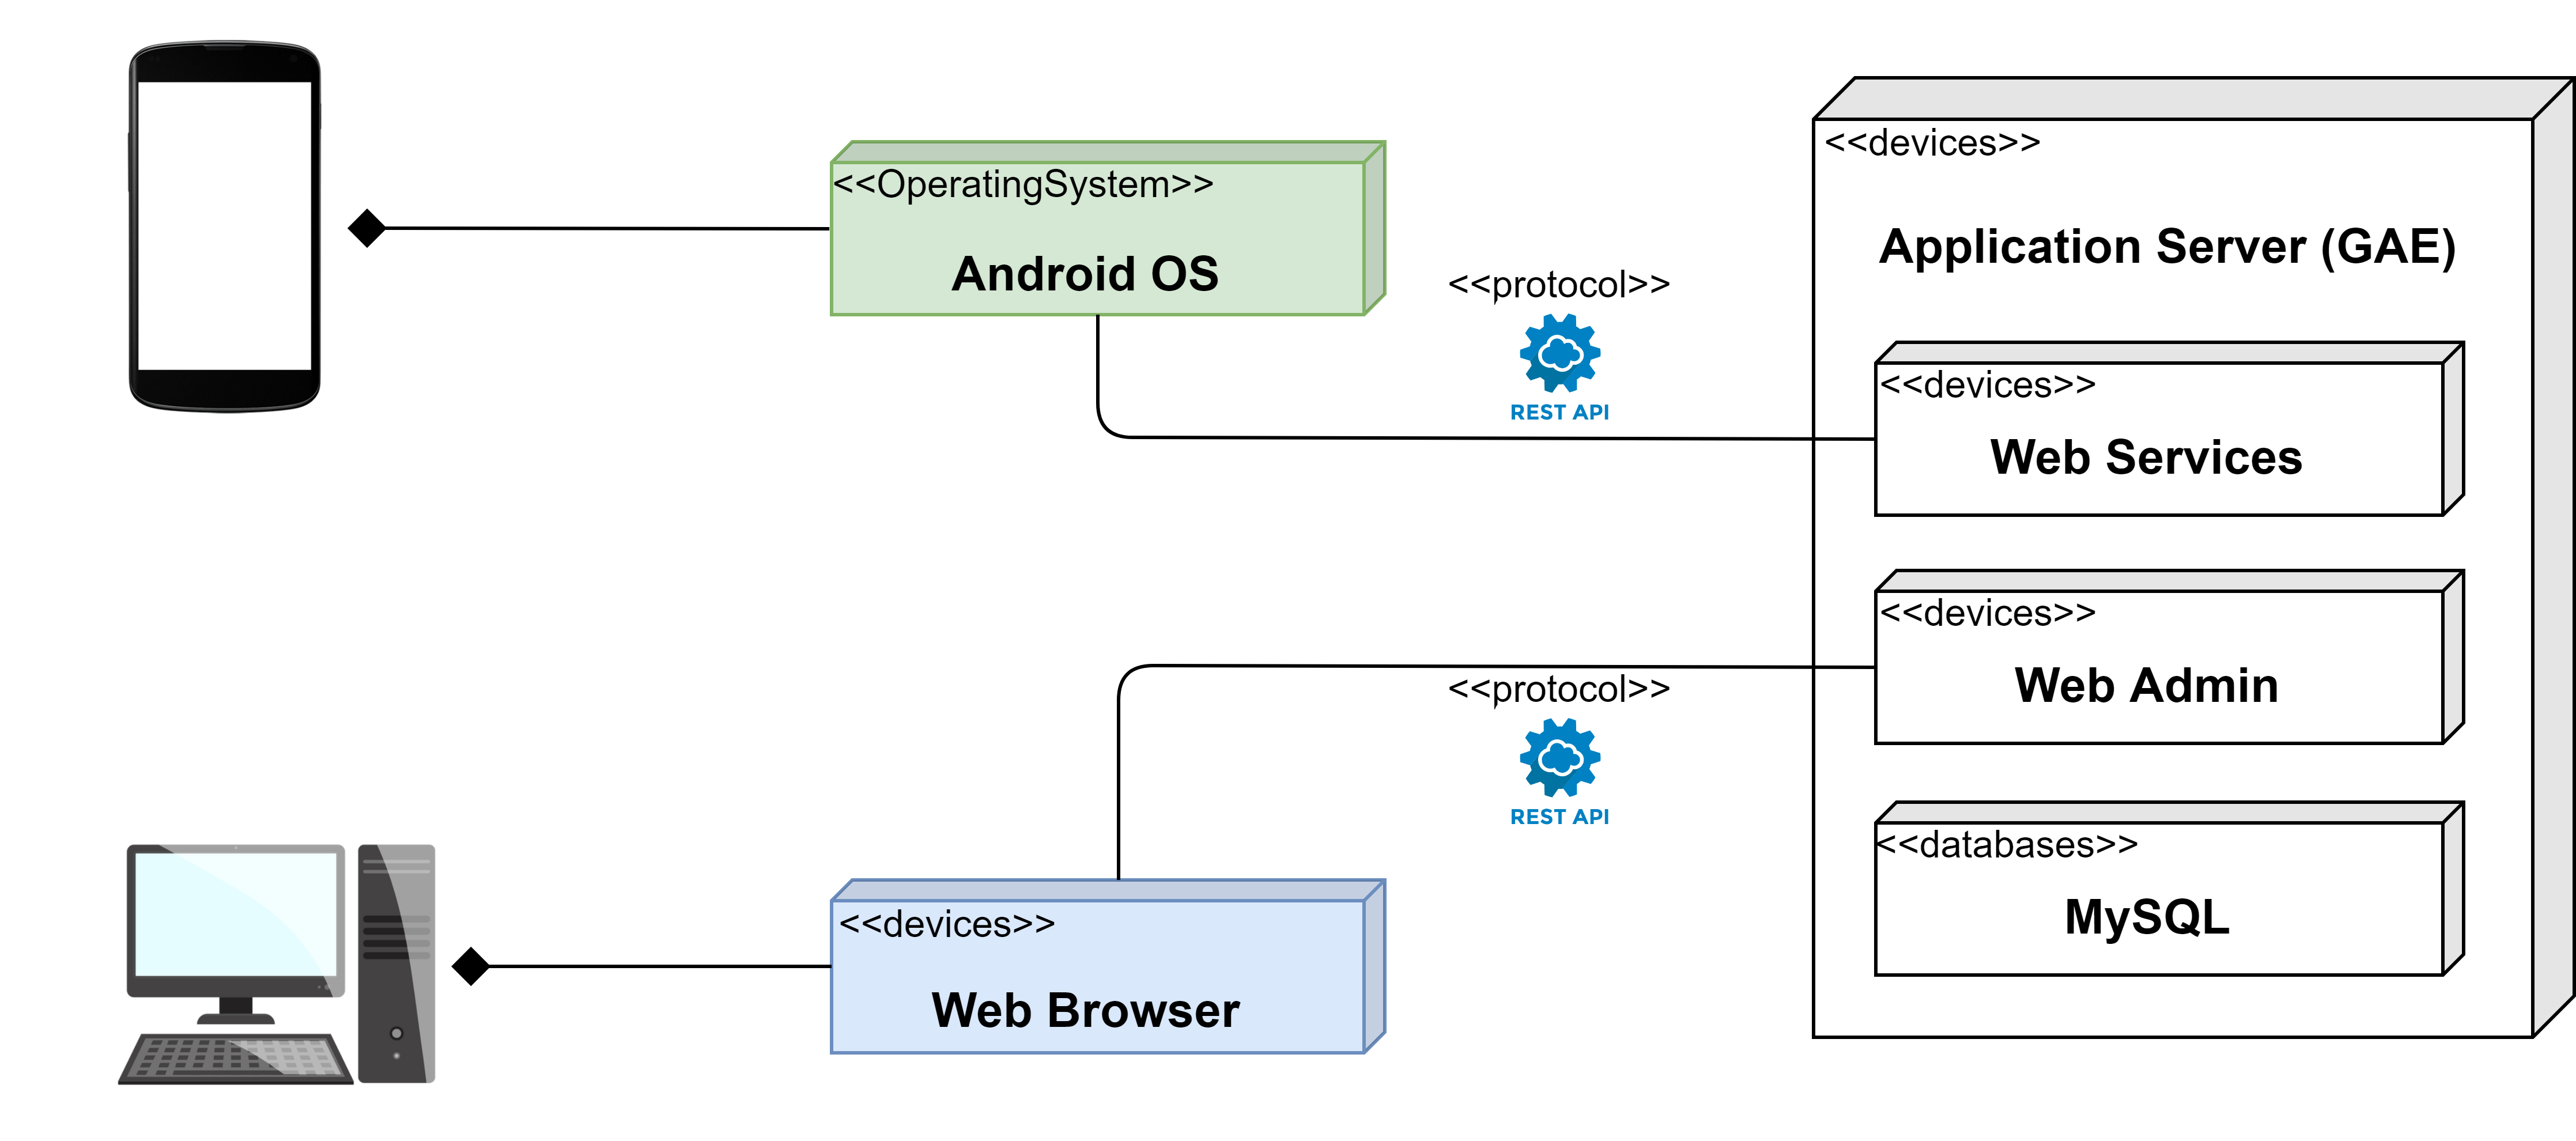
\includegraphics [width = 13.5cm, height= 5.5cm]{gambar/model/deployment-diagram-absensi}
						%\caption{Diagram Deployment Aplikasi Kehadiran Dosen dan Mahasiswa}
					%\label{deploymentabsensi}
					%\end{figure}
   			%\end{enumerate}
 	
	Tahap kedua adalah merancang tampilan antar muka pengguna (\textit{user interface}) sebagai mekanisme komunikasi dengan sistem. Antar muka dari sistem yang telah dibangun adalah sebagai berikut:
		\begin{enumerate}[a.]
		
		\item Antar Muka Aplikasi Mapping
		
		\par Gambar \ref{aplikasimappingbagian1} menampilkan halaman ketika menggunakan aplikasi, kemudian akan muncul notifikasi permintaan izin mengakses lokasi pada perangkat untuk pemindaian kekuatan sinyal Bluetooth. Halaman beranda menampilkan informasi nama ruangan, nama \textit{device} Bluetooth, RSSI dan MAC Address Bluetooth apabila proses pemindaian telah selesai dilakukan serta beberapa tombol untuk memulai proses pemindaian, tombol untuk menyimpan data hasil pemindaian, dan tombol untuk menampilkan data hasil pemindaian.  
				
		\vspace{-0cm}
	\begin{figure} [H]
	\begin{subfigure}{.5\textwidth}
  		\centering
  		% include first image
  		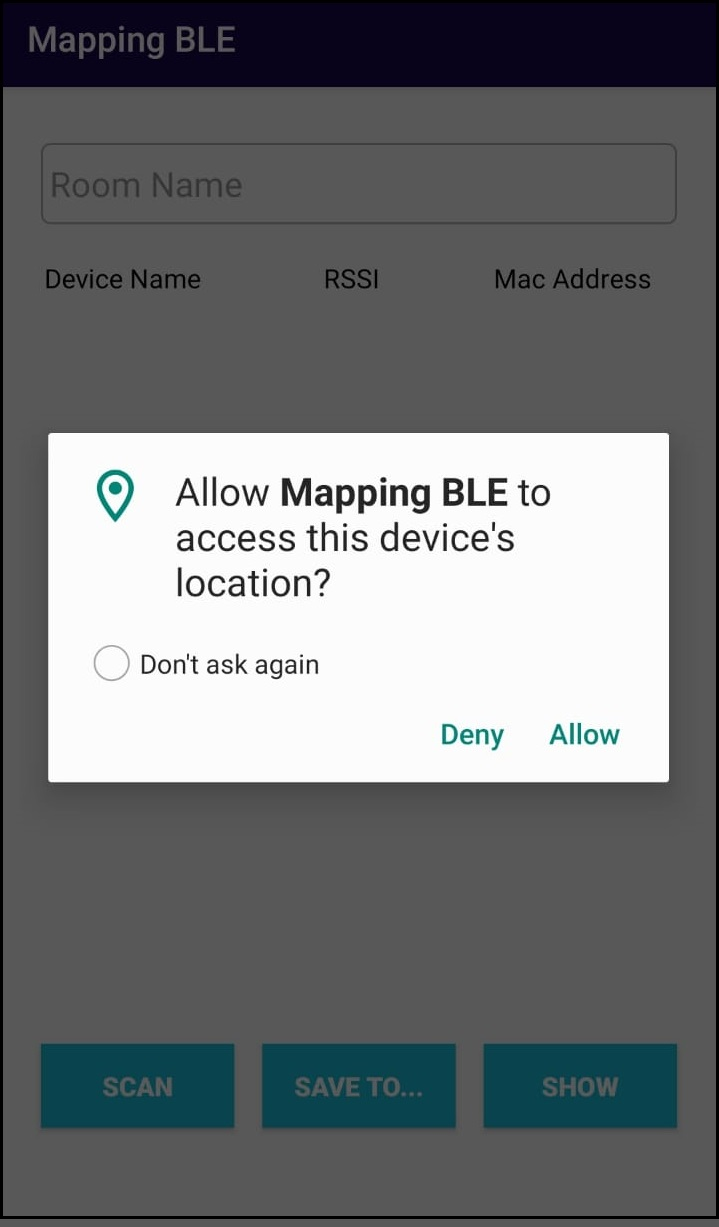
\includegraphics[width=.5\linewidth]{gambar/android/mapping-permission}  
  		\caption{Izin mengakses lokasi}
	\end{subfigure}
	\begin{subfigure}{.5\textwidth}
  		\centering
  		% include second image
		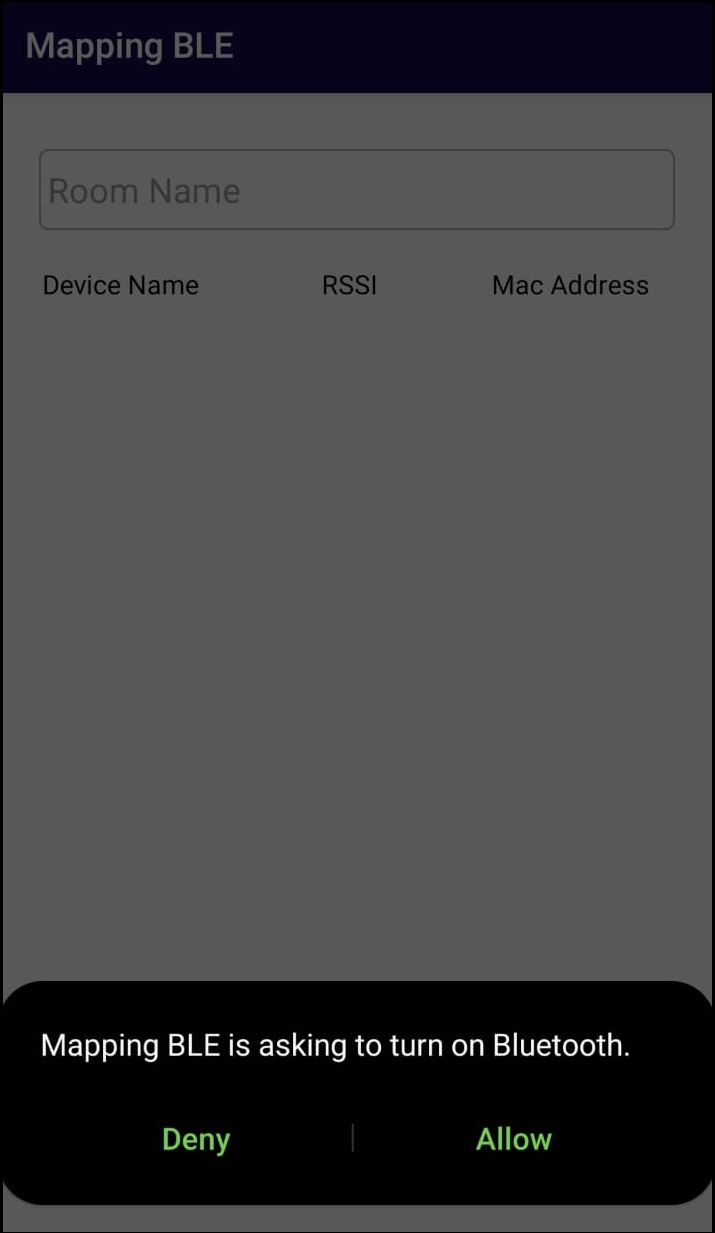
\includegraphics[width=.5\linewidth]{gambar/android/mapping-bluetooth}  
  		\caption{Menghidupkan Bluetooth}
	\end{subfigure}
		\vspace{1cm}
		\newline
	\begin{subfigure}{.5\textwidth}
  		\centering
		 % include third image
	  	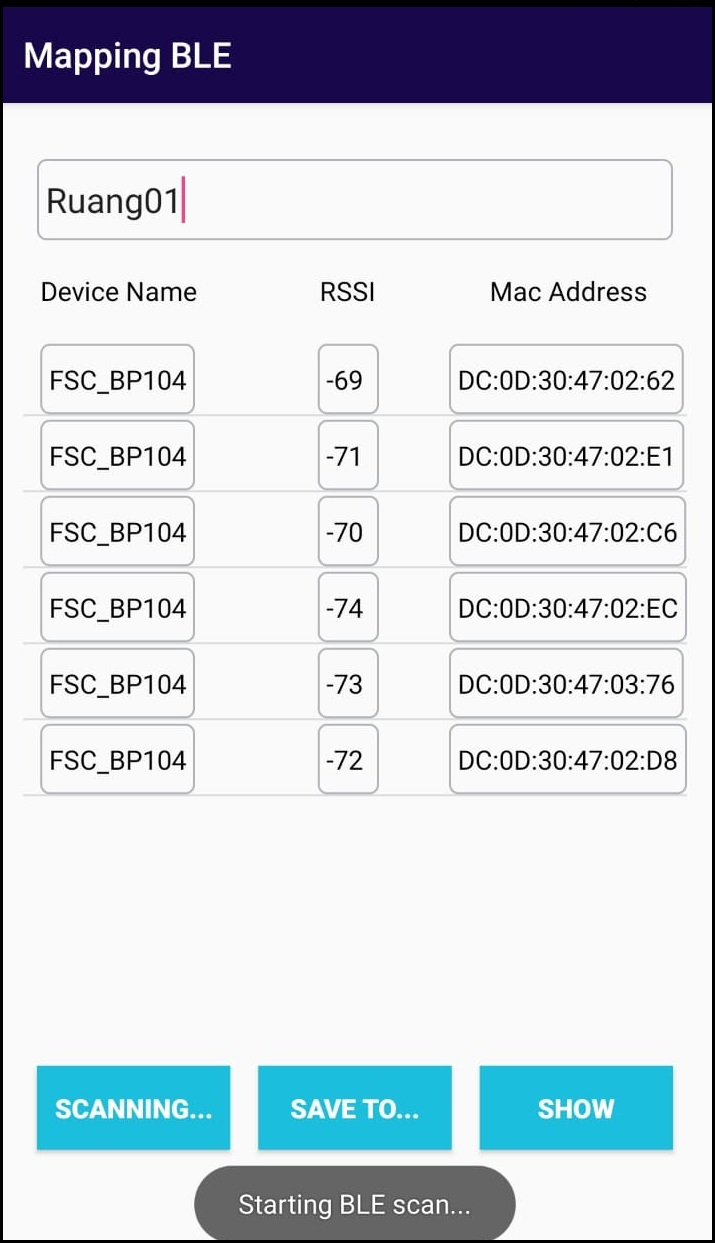
\includegraphics[width=.5\linewidth]{gambar/android/mapping-scanning}  
  		\caption{Proses pemindaian kekuatan sinyal}
	\end{subfigure}
	\begin{subfigure}{.5\textwidth}
  		\centering
  		% include fourth image
  		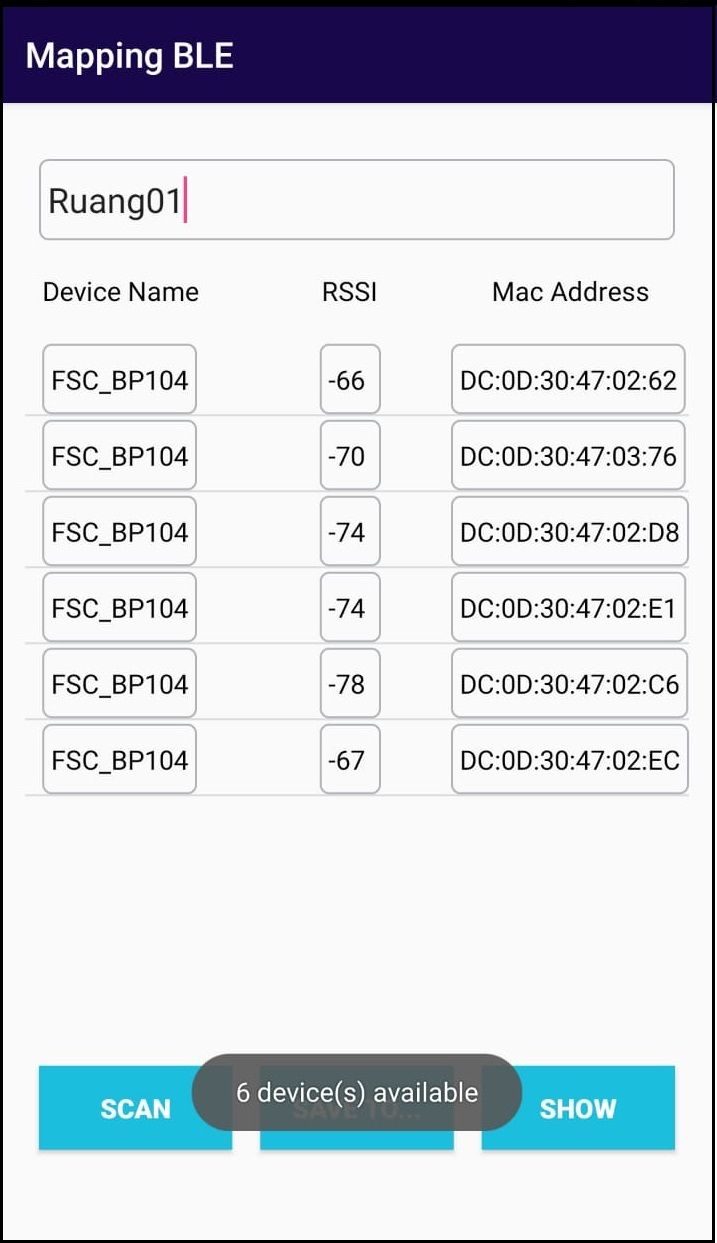
\includegraphics[width=.5\linewidth]{gambar/android/mapping-finish-scan}  
  		\caption{Selesai proses pemindaian}
	\end{subfigure}
		\vspace{0.5cm}
		\caption{Tampilan Halaman Aplikasi Mapping (Bagian 1)}
	\label{aplikasimappingbagian1}
	\end{figure}
	
	\par Apabila pengguna menekan tombol \textbf{save to}, akan muncul \textit{pop up} dimana pengguna dapat memilih tabel penyimpanan data hasil pemindaian, yaitu: tabel \textit{reference point} urut dan tabel \textit{reference point} acak. Jika pengguna menekan tombol \textbf{show data}, akan muncul \textit{pop up} dimana pengguna dapat memilih tabel untuk data yang ingin ditampilkan, kemudian pengguna akan diarahkan ke halaman daftar data hasil pemindaian kekuatan sinyal yang telah disimpan sebelumnya. Jika pengguna ingin menghapus sebuah data, pengguna harus menekan tombol \textit{icon} tong sampah dan lakukan konfirmasi. Fitur-fitur tersebut dapat dilihat pada Gambar \ref{aplikasimappingbagian2}.   
	
	\vspace{-0cm}
	\begin{figure} [H]
	\begin{subfigure}{.5\textwidth}
  		\centering
  		% include first image
  		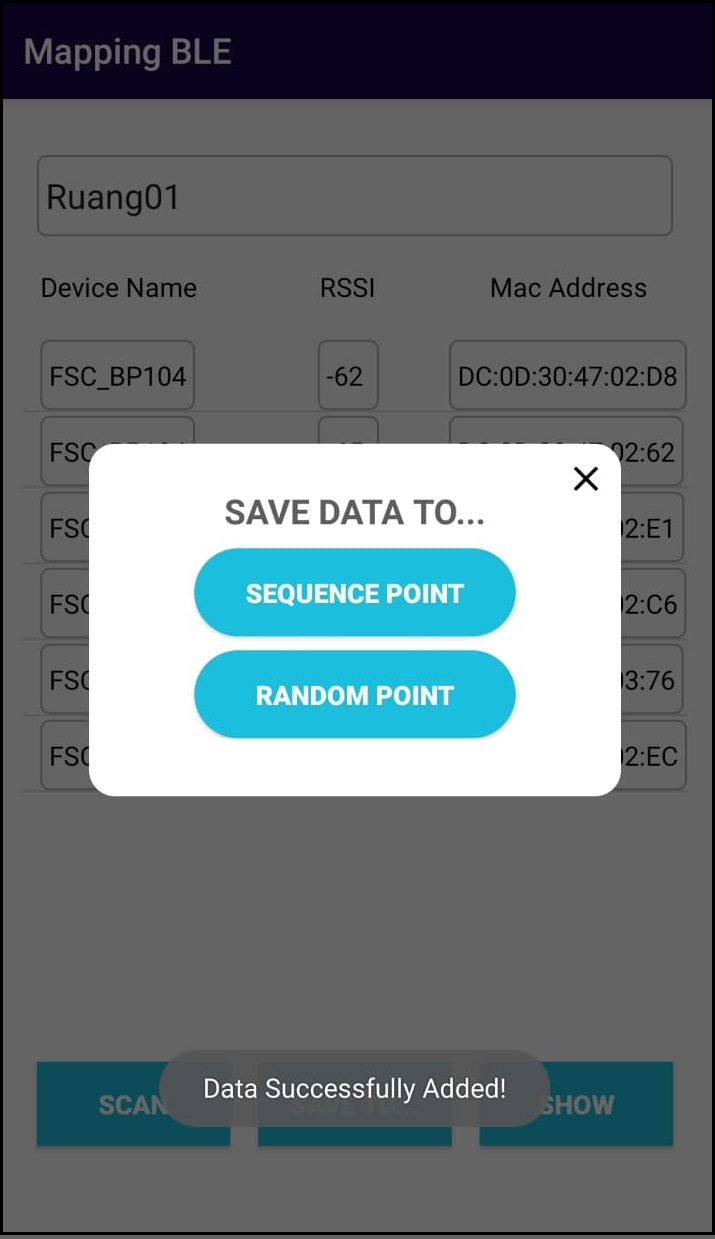
\includegraphics[width=.5\linewidth]{gambar/android/mapping-save-data}  
  		\caption{Simpan hasil pemindaian}
	\end{subfigure}
	\begin{subfigure}{.5\textwidth}
  		\centering
  		% include second image
  		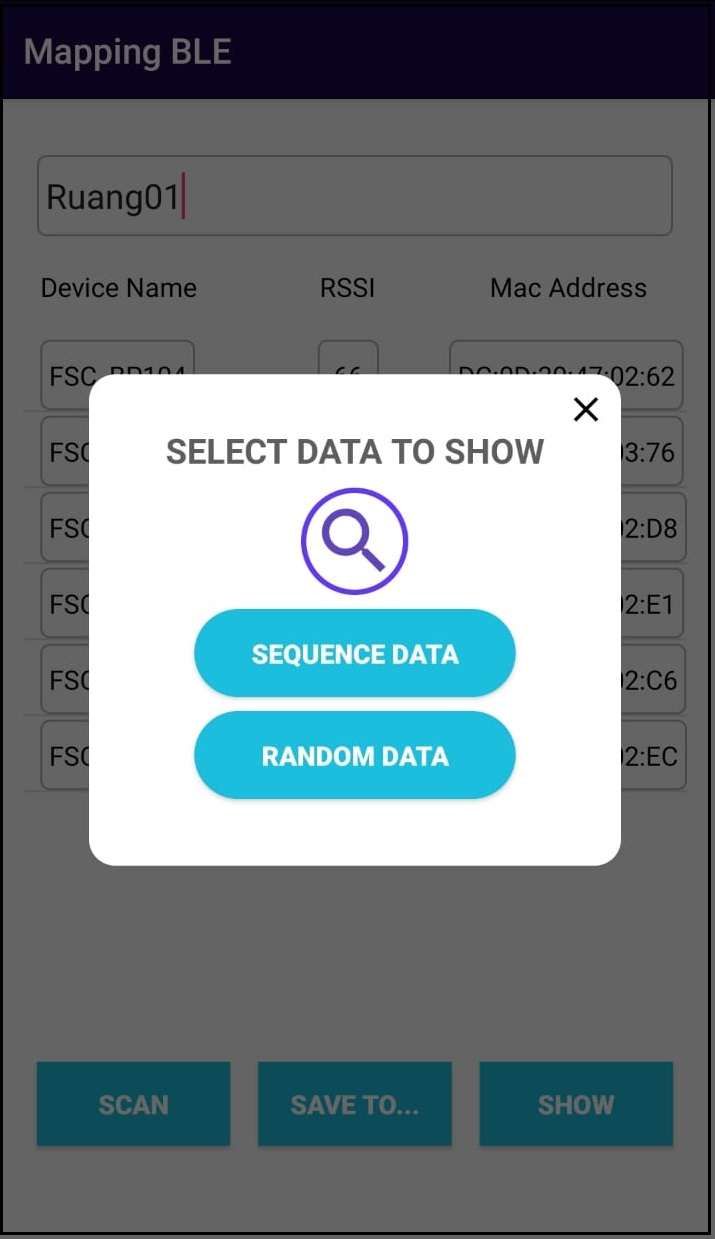
\includegraphics[width=.5\linewidth]{gambar/android/mapping-show-data}  
  		\caption{Pilihan menampilkan data}
	\end{subfigure}
	\vspace{1cm}
	\newline
	\begin{subfigure}{.5\textwidth}
  		\centering
  		% include third image
  		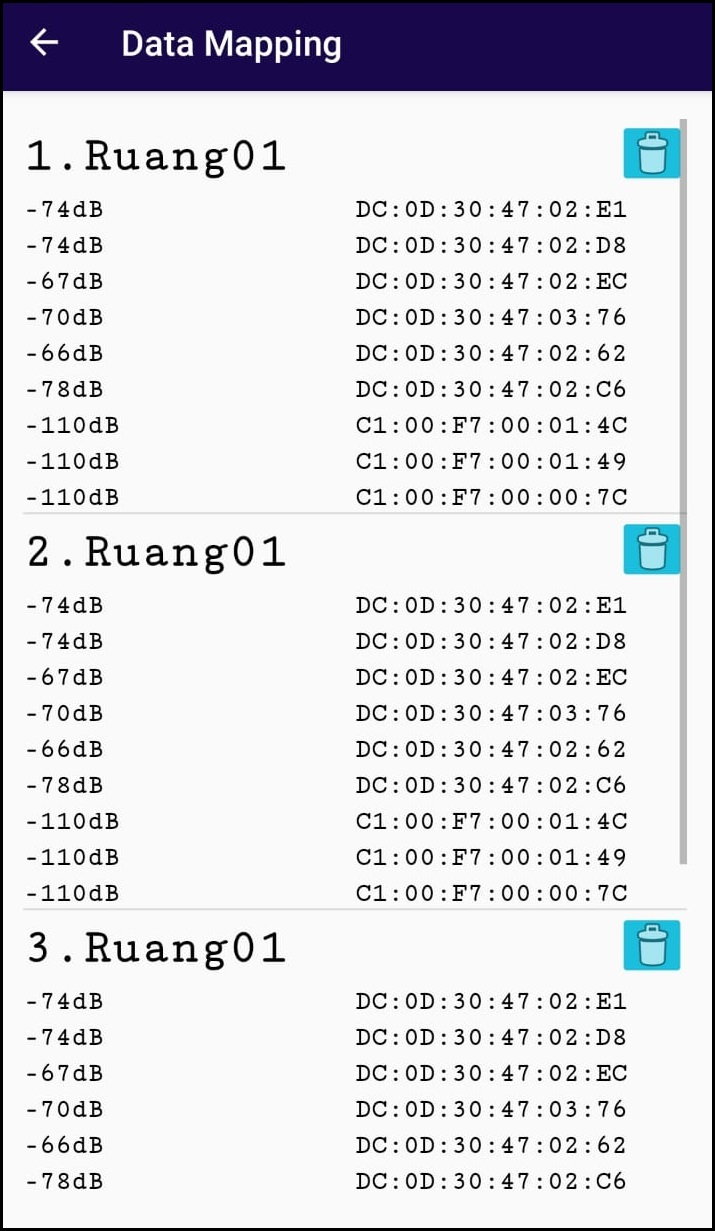
\includegraphics[width=.5\linewidth]{gambar/android/mapping-data-list}  
  		\caption{Menampilkan data yang disimpan}
	\end{subfigure}
	\begin{subfigure}{.5\textwidth}
  		\centering
  		% include fourth image
  		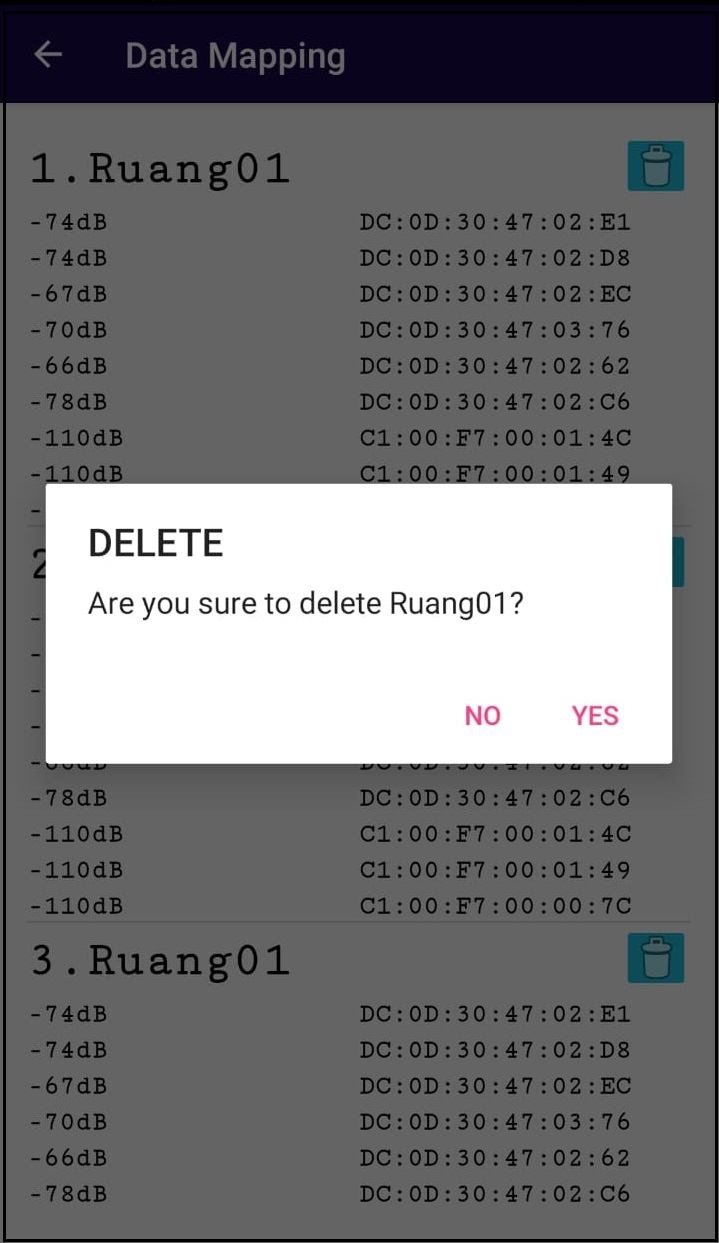
\includegraphics[width=.5\linewidth]{gambar/android/mapping-delete}
  		\caption{Hapus data}
	\end{subfigure}
		\vspace{0.5cm}
		\caption{Tampilan Halaman Aplikasi Mapping (Bagian 2)}
	\label{aplikasimappingbagian2}
	\end{figure}
	%Akhir Gambar Aplikasi Mapping%
	
\vspace{1cm}
		\item Antar Muka Aplikasi Kehadiran Dosen
		
		\par Gambar \ref{aplikasidosenbagian1} memperlihatkan ketika dosen belum melakukan \textit{log in}, aplikasi akan menampilkan \textit{landing page} yang berisi langkah-langkah penggunaan aplikasi, selanjutnya dosen akan diarahkan ke halaman \textit{log in}. Untuk melakukan \textit{log in}, dosen diminta untuk memasukkan Nomor Induk Pegawai (NIP) dan kata sandi yang sesuai dengan Sistem Kepegawaian (SIMPEG) Unsyiah. Setelah itu, dosen akan diarahkan ke halaman beranda apabila telah berhasil melakukan \textit{log in}. Pada halaman beranda, terdapat informasi data diri dosen serta mata kuliah yang diajarkan oleh dosen yang bersangkutan. Jika dosen menekan salah-satu mata kuliah, dosen akan diarahkah ke halaman informasi mata kuliah tersebut.
	\vspace{-0cm}
	\begin{figure} [H]
	\begin{subfigure}{.5\textwidth}
  		\centering
  		% include first image
  		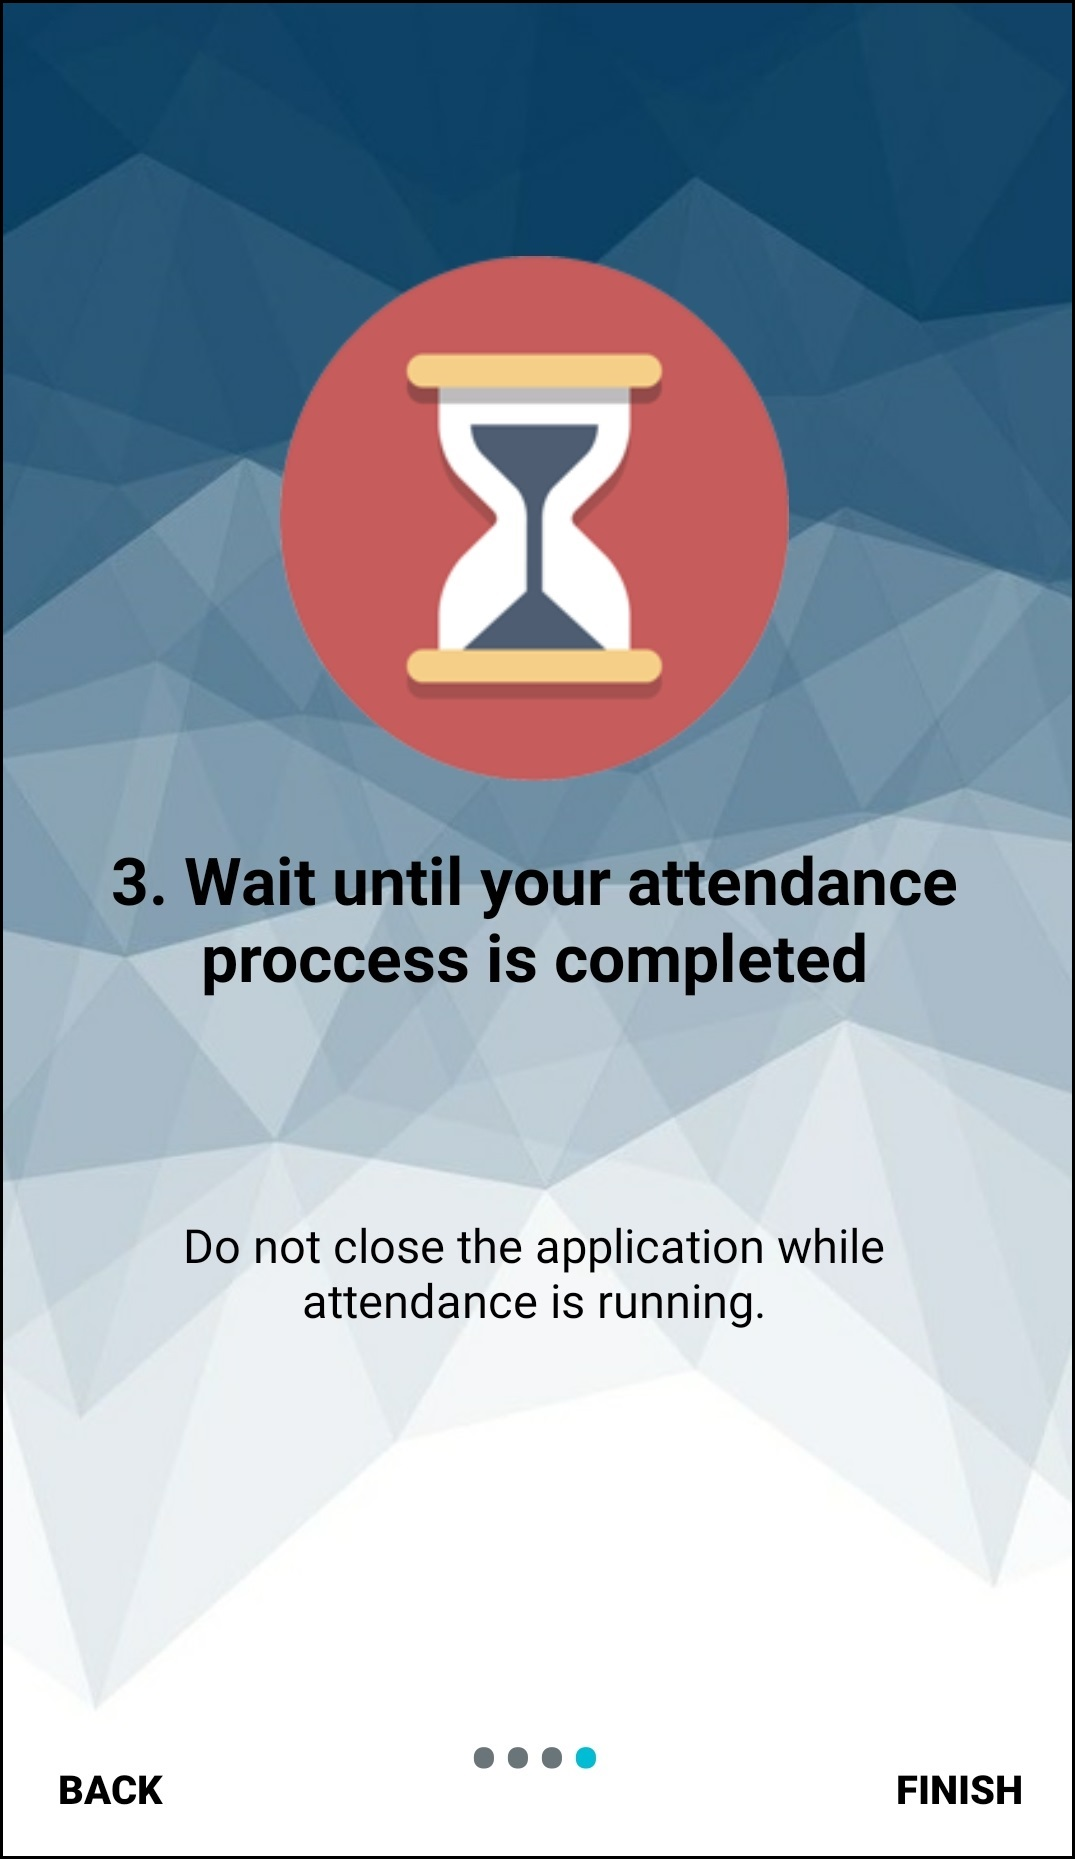
\includegraphics[width=.5\linewidth]{gambar/android/dosen-1}  
  		\caption{\textit{Landing page}}
	\end{subfigure}
	\begin{subfigure}{.5\textwidth}
  		\centering
  		% include second image
		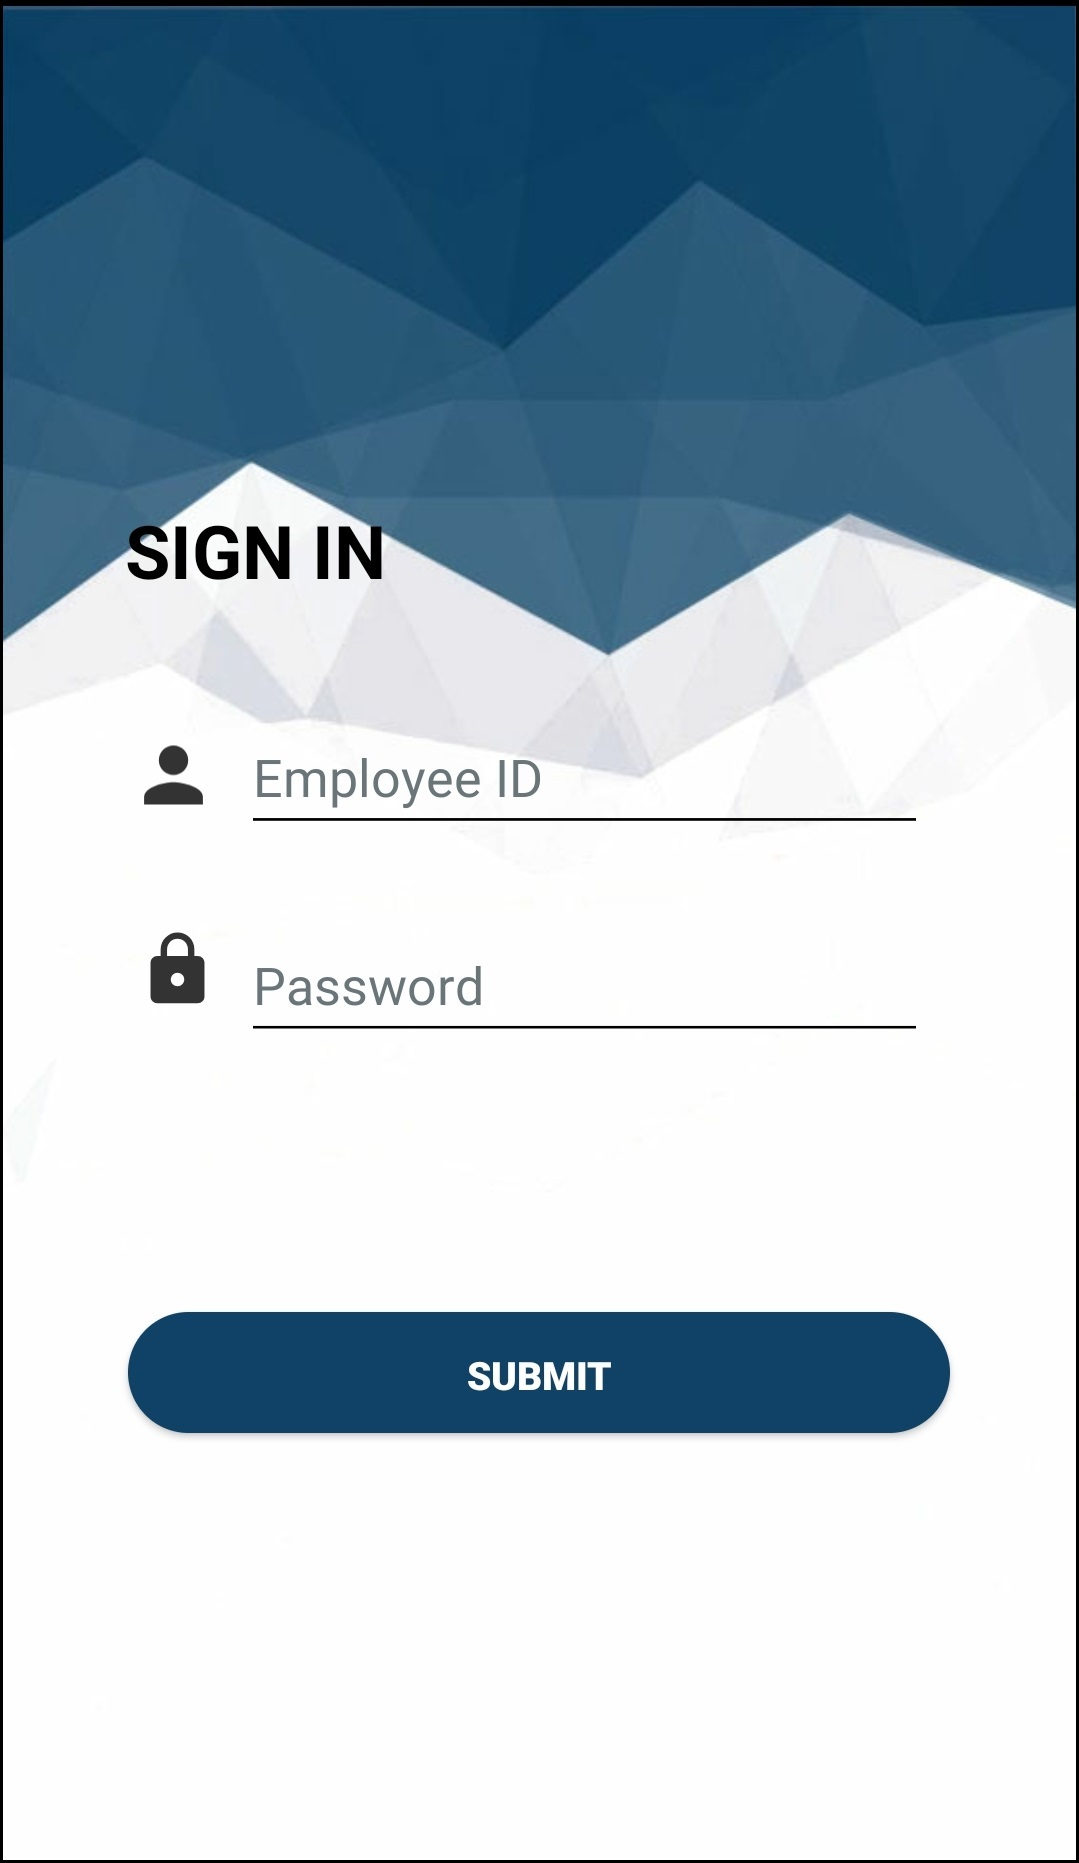
\includegraphics[width=.5\linewidth]{gambar/android/dosen-2}  
  		\caption{\textit{Log in}}
	\end{subfigure}
		\vspace{1cm}
		\newline
	\begin{subfigure}{.5\textwidth}
  		\centering
		 % include third image
	  	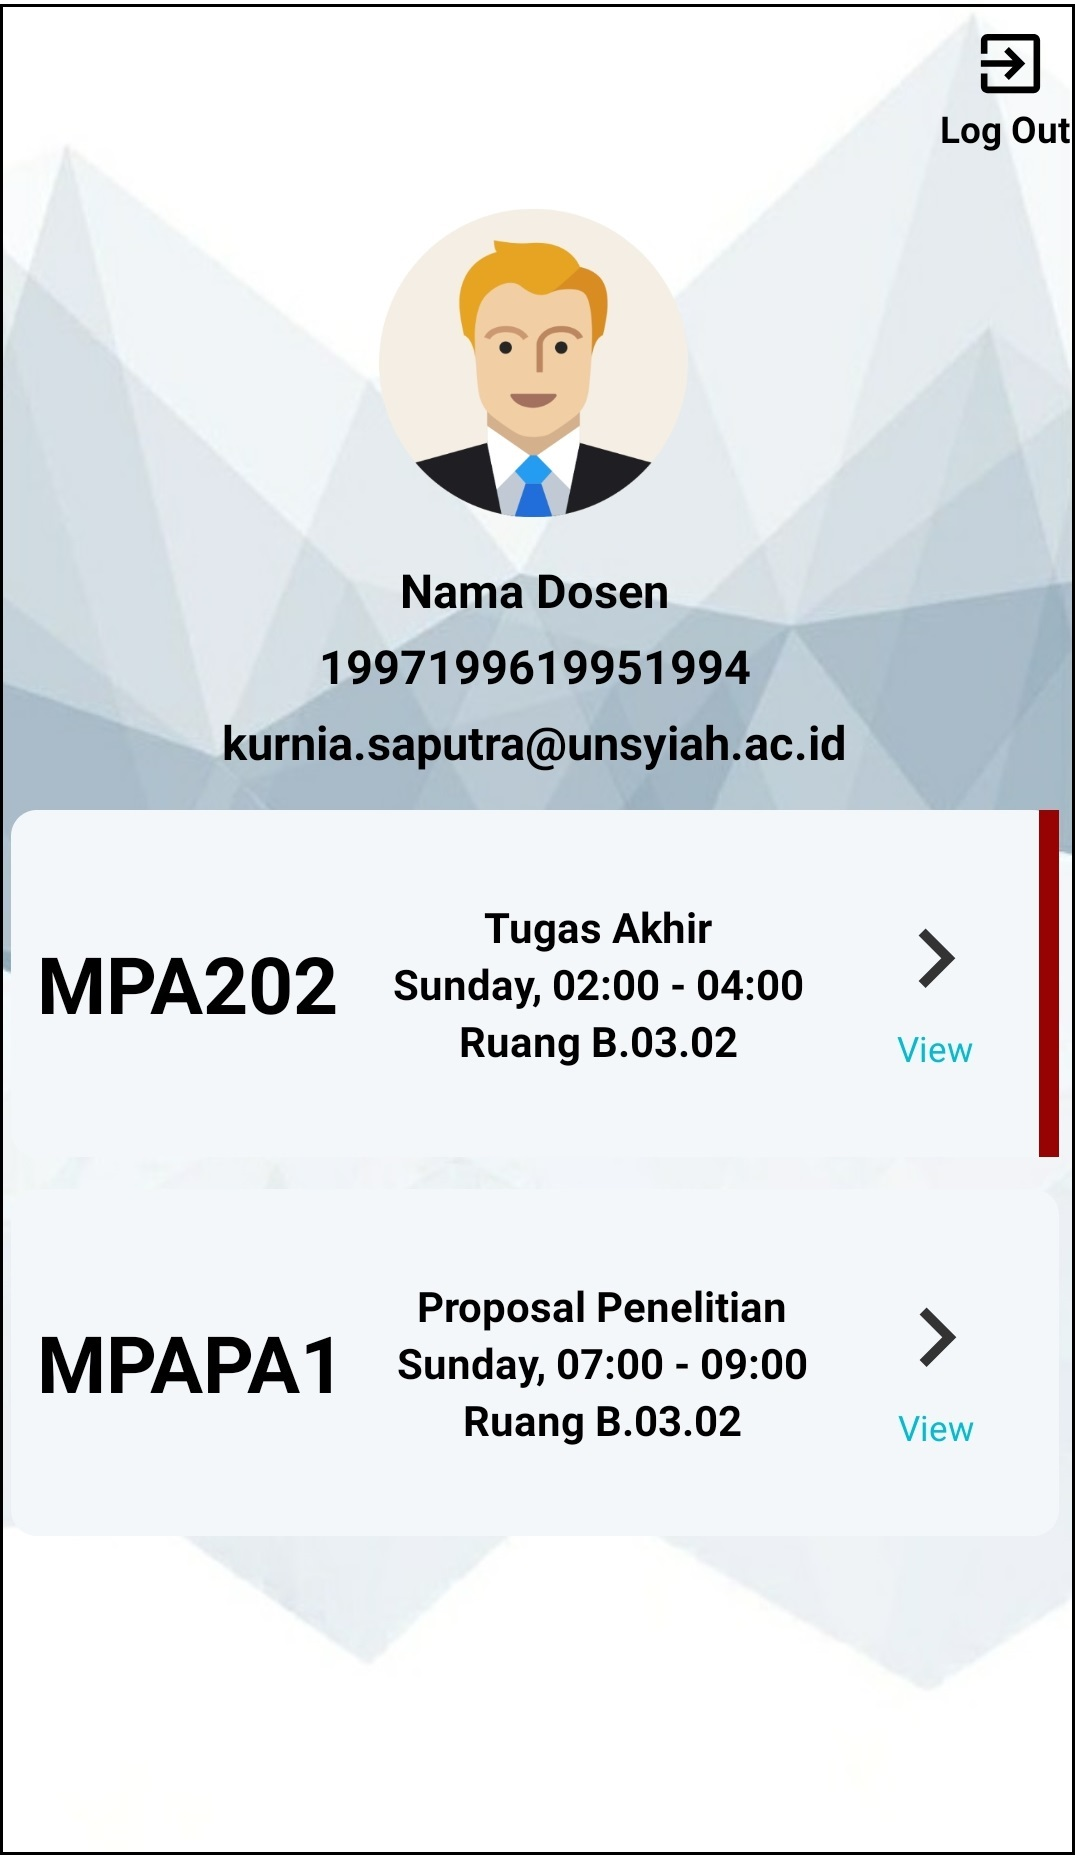
\includegraphics[width=.5\linewidth]{gambar/android/dosen-3}  
  		\caption{Beranda}
	\end{subfigure}
	\begin{subfigure}{.5\textwidth}
  		\centering
  		% include fourth image
  		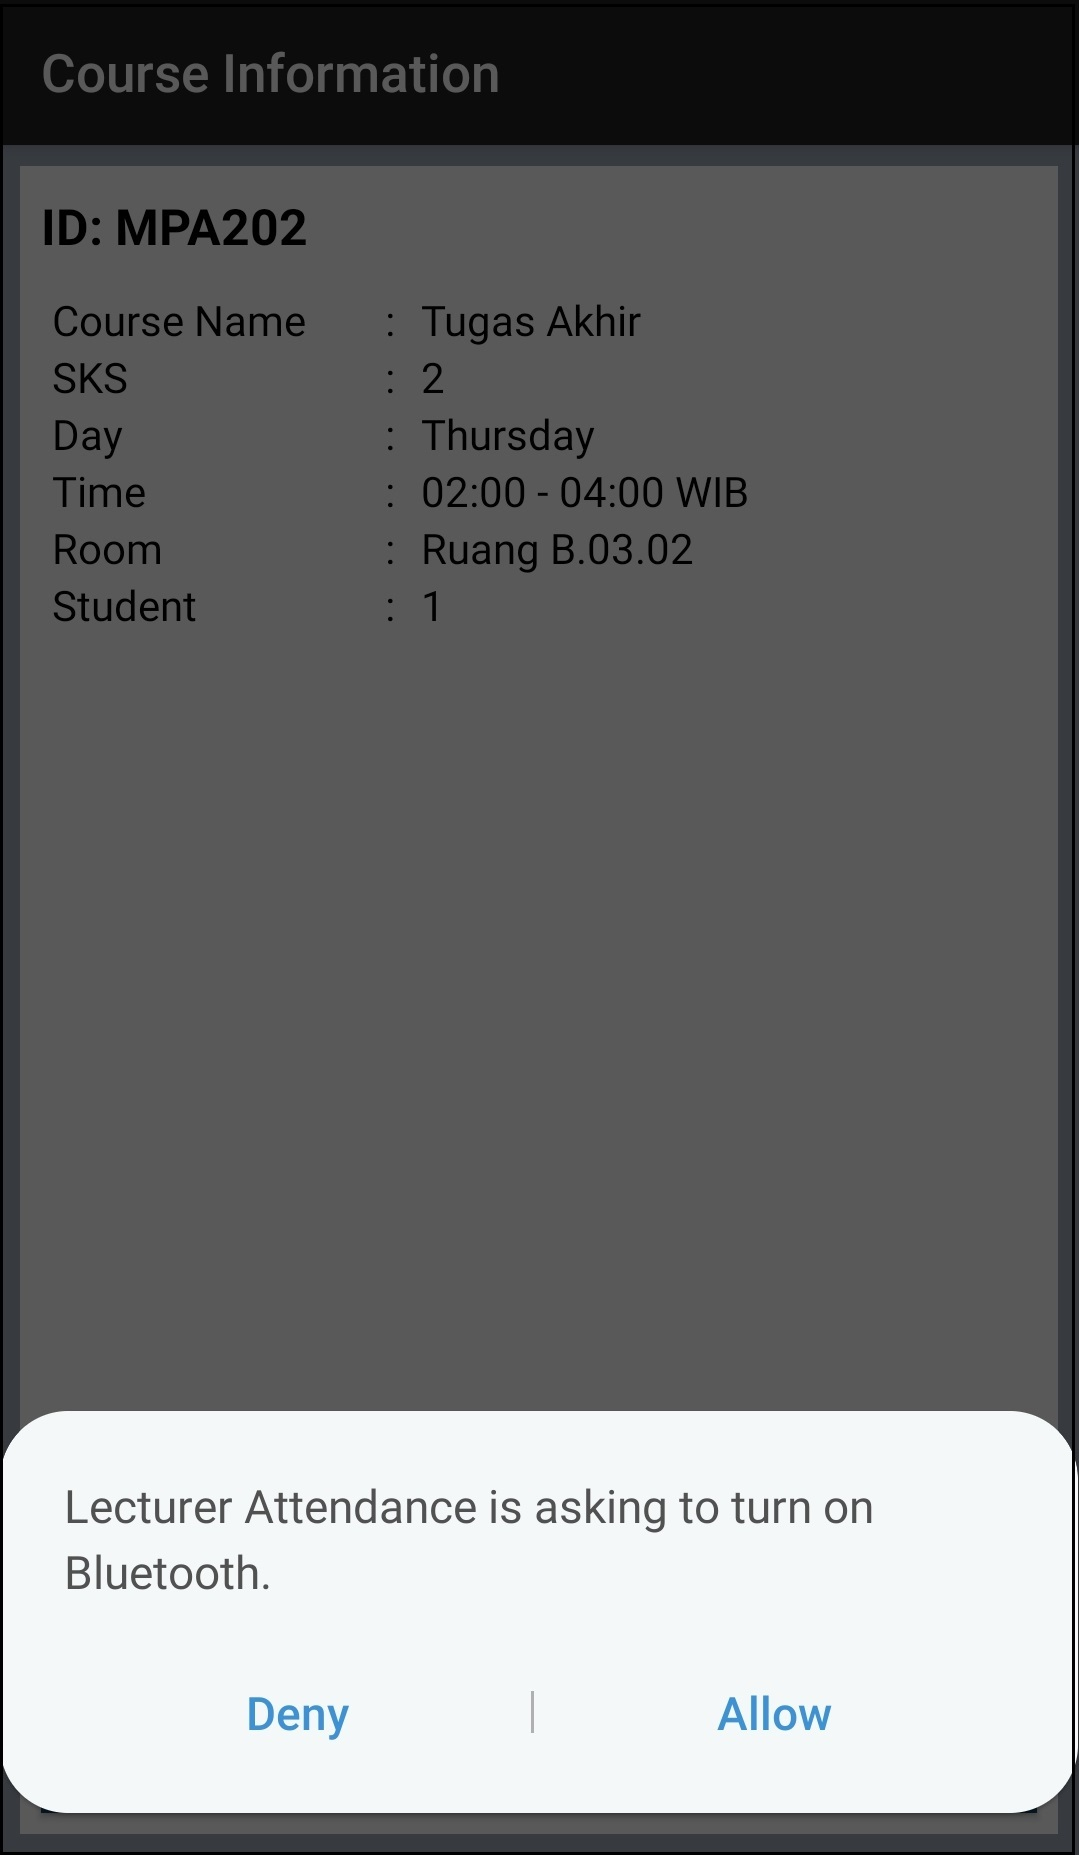
\includegraphics[width=.5\linewidth]{gambar/android/dosen-4}  
  		\caption{Informasi matakuliah}
	\end{subfigure}
		\vspace{0.5cm}
		\caption{Tampilan Halaman Aplikasi Kehadiran Dosen (Bagian 1)}
	\label{aplikasidosenbagian1}
	\end{figure}
	
\vspace{0.5cm}
	\par Gambar \ref{aplikasidosenbagian2} memperlihatkan ketika dosen telah berada di halaman informasi mata kuliah Kemudian, aplikasi akan menampilkan notifikasi untuk menghidupkan Bluetooth apabila Bluetooth pada perangkat belum hidup. Terdapat dua tombol yaitu tombol \textbf{show students} untuk melihat daftar mahasiswa yang mengambil mata kuliah tersebut dan tombol \textbf{start attendance} untuk memulai proses kehadiran. Aplikasi akan melakukan klasifikasi dengan metode K-NN untuk memprediksi lokasi dosen.
	
	\vspace{-0cm}
	\begin{figure} [H]
	\begin{subfigure}{.5\textwidth}
  		\centering
  		% include first image
  		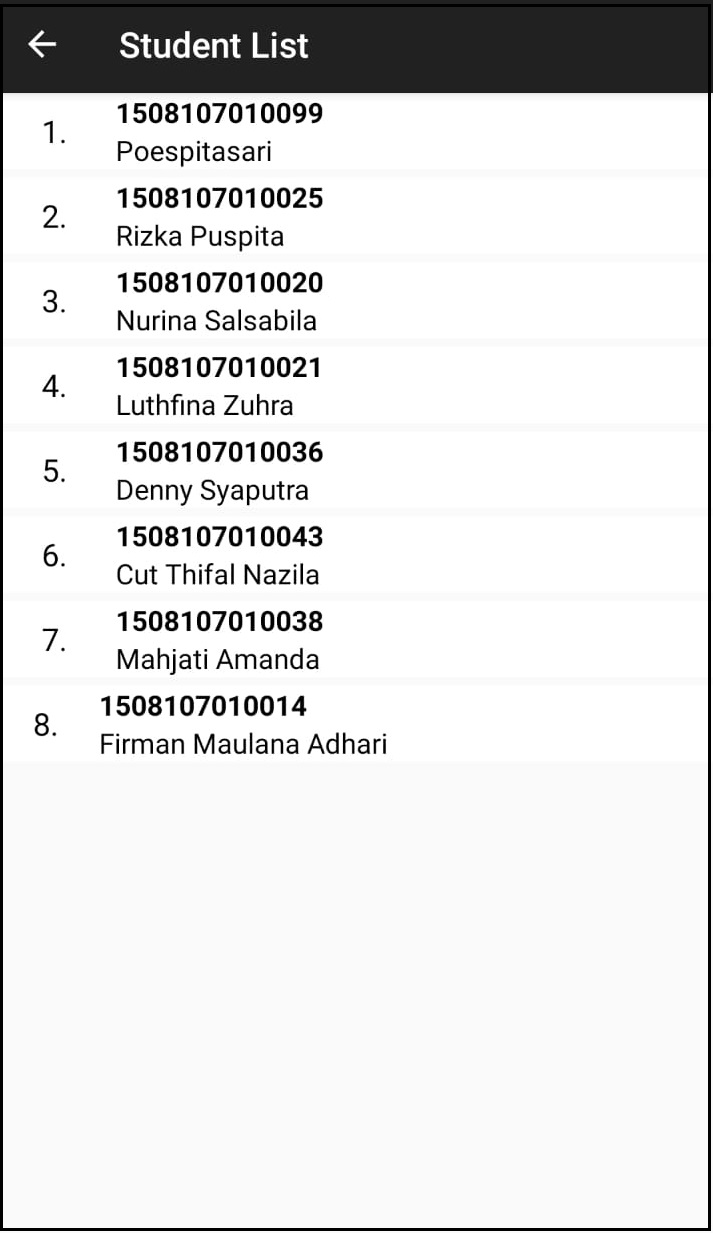
\includegraphics[width=.5\linewidth]{gambar/android/dosen-5}  
  		\caption{Daftar mahasiswa}
	\end{subfigure}
	\begin{subfigure}{.5\textwidth}
  		\centering
  		% include second image
  		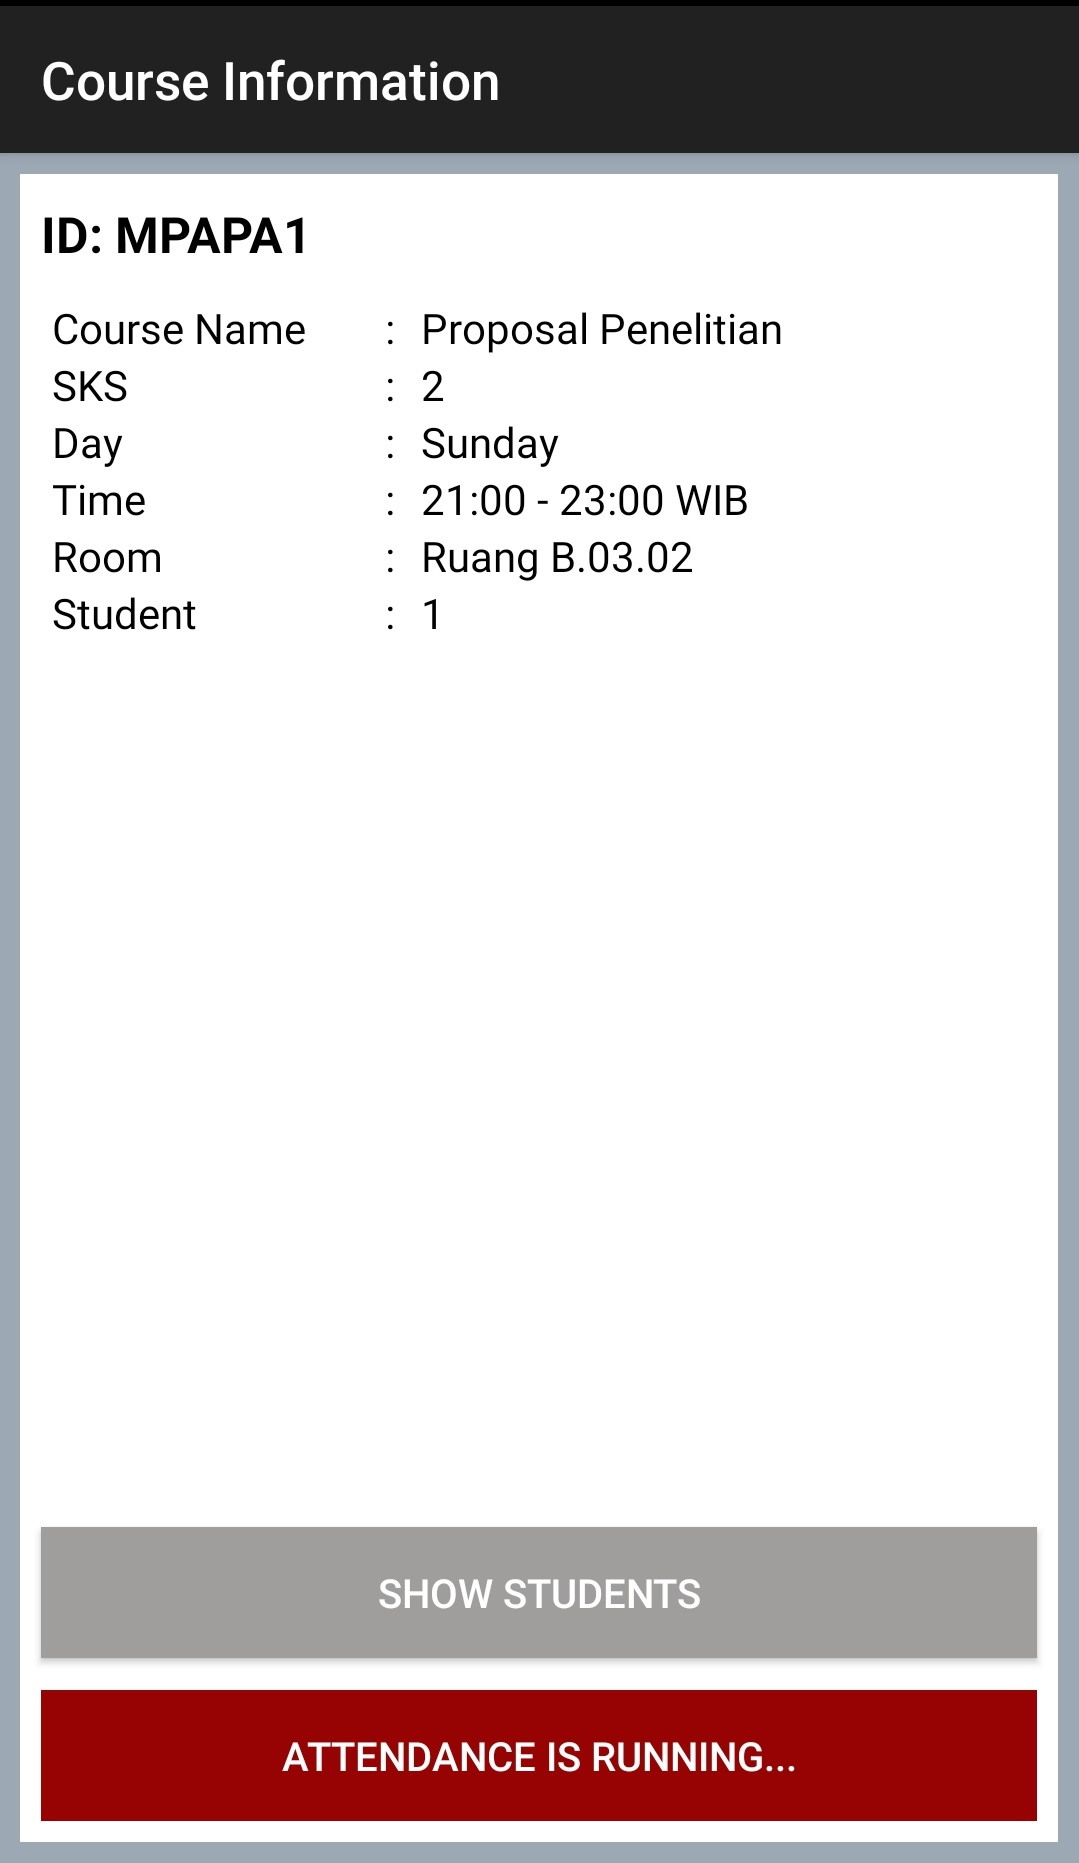
\includegraphics[width=.5\linewidth]{gambar/android/dosen-6}  
  		\caption{Proses kehadiran sedang berjalan}
	\end{subfigure}
	\vspace{1cm}
	\newline
	\begin{subfigure}{.5\textwidth}
  		\centering
  		% include third image
  		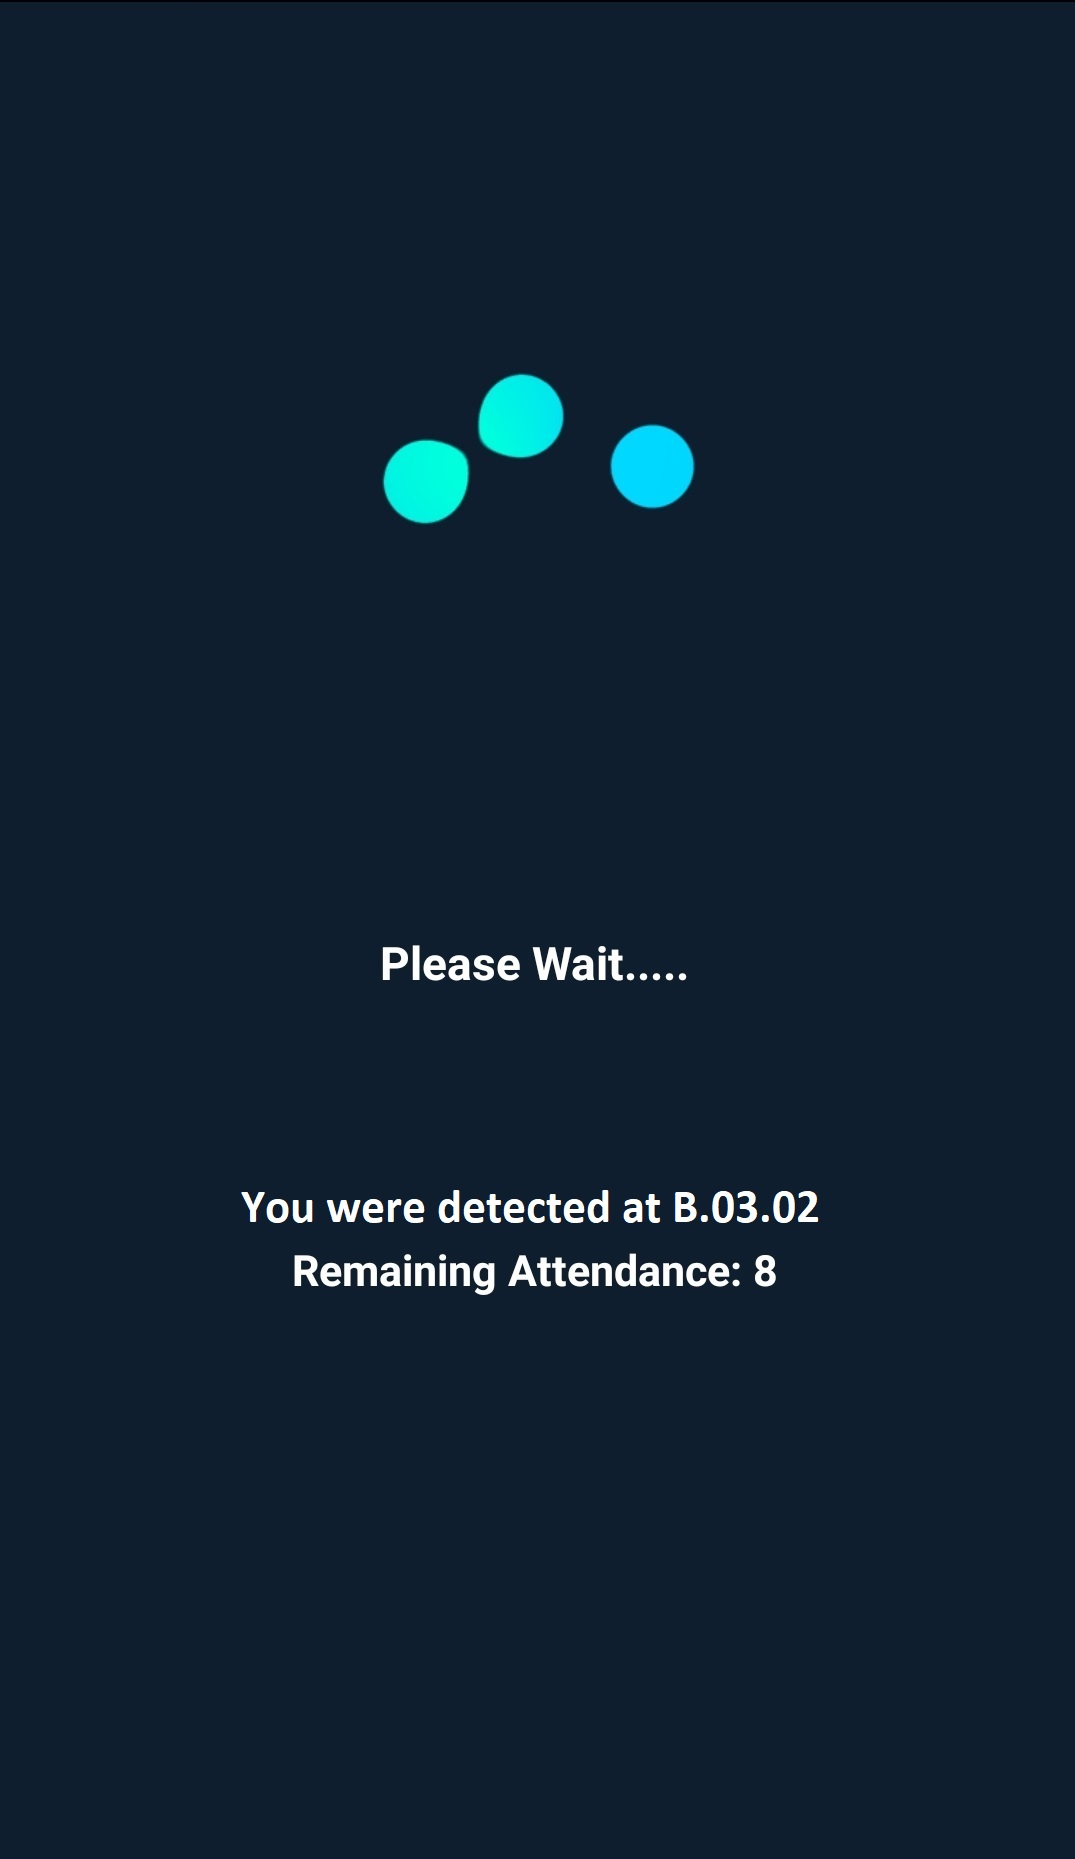
\includegraphics[width=.5\linewidth]{gambar/android/dosen-7}  
  		\caption{Dosen diprediksi di dalam kelas}
	\end{subfigure}
	\begin{subfigure}{.5\textwidth}
  		\centering
  		% include fourth image
  		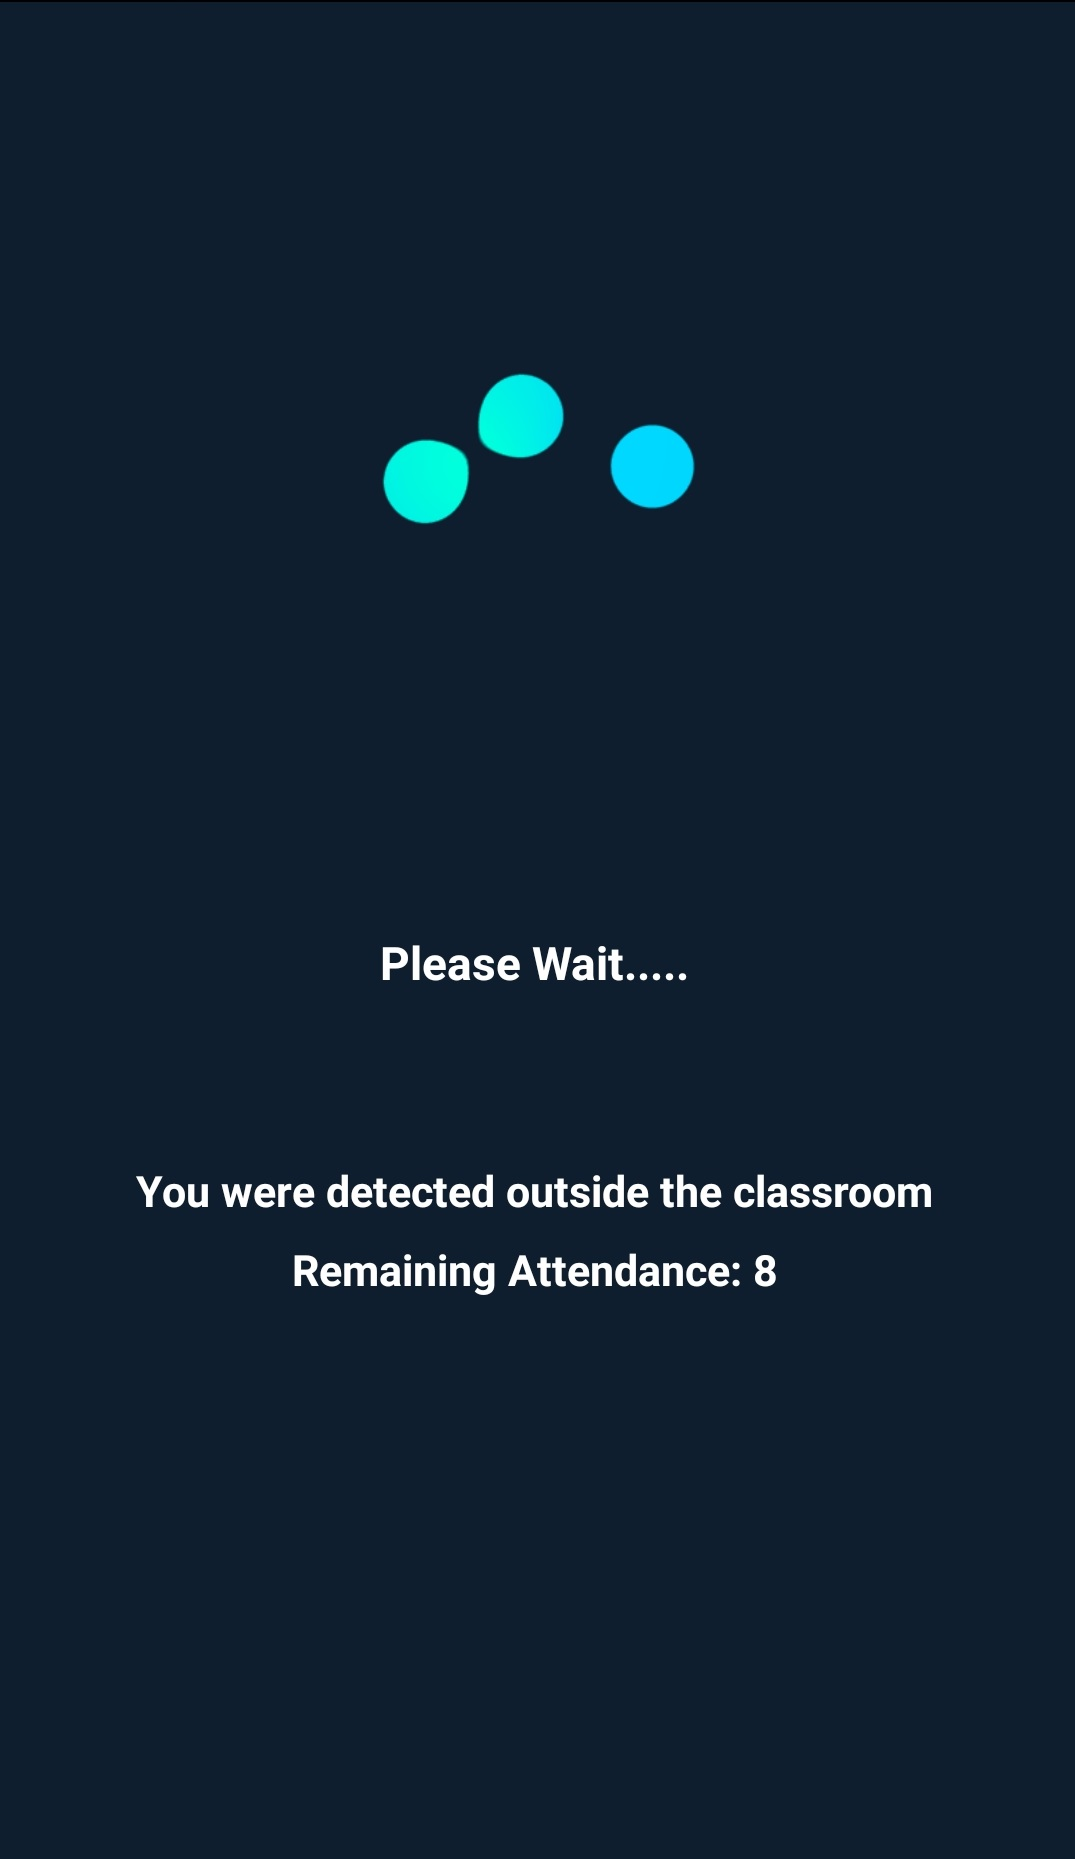
\includegraphics[width=.5\linewidth]{gambar/android/dosen-8}  
  		\caption{Dosen diprediksi di luar kelas}
	\end{subfigure}
		\vspace{0.5cm}
		\caption{Tampilan Halaman Aplikasi Kehadiran Dosen (Bagian 2)}
	\label{aplikasidosenbagian2}
	\end{figure}
	%Akhir Gambar Aplikasi Kehadiran Dosen%
	
	\item Antar Muka Aplikasi Kehadiran Mahasiswa
	
	\par Gambar \ref{aplikasimahasiswabagian1} memperlihatkan ketika mahasiswa belum melakukan \textit{log in}, aplikasi akan menampilkan \textit{landing page} yang berisi langkah-langkah penggunaan aplikasi, lalu mahasiswa akan diarahkan ke halaman \textit{log in}. Untuk melakukan \textit{log in}, mahasiswa diminta untuk memasukkan Nomor Pokok Mahasiswa (NPM) dan kata sandi yang sesuai dengan KRS Online Unsyiah. Setelah itu, mahasiswa akan diarahkan ke halaman beranda apabila telah berhasil melakukan \textit{log in}. Pada halaman beranda, terdapat beberapa menu seperti menu profil, menu daftar mata kuliah dan menu tentang aplikasi, serta informasi mata kuliah hari ini. 
	
	\vspace{-0cm}
	\begin{figure} [H]
	\begin{subfigure}{.5\textwidth}
  		\centering
  		% include first image
  		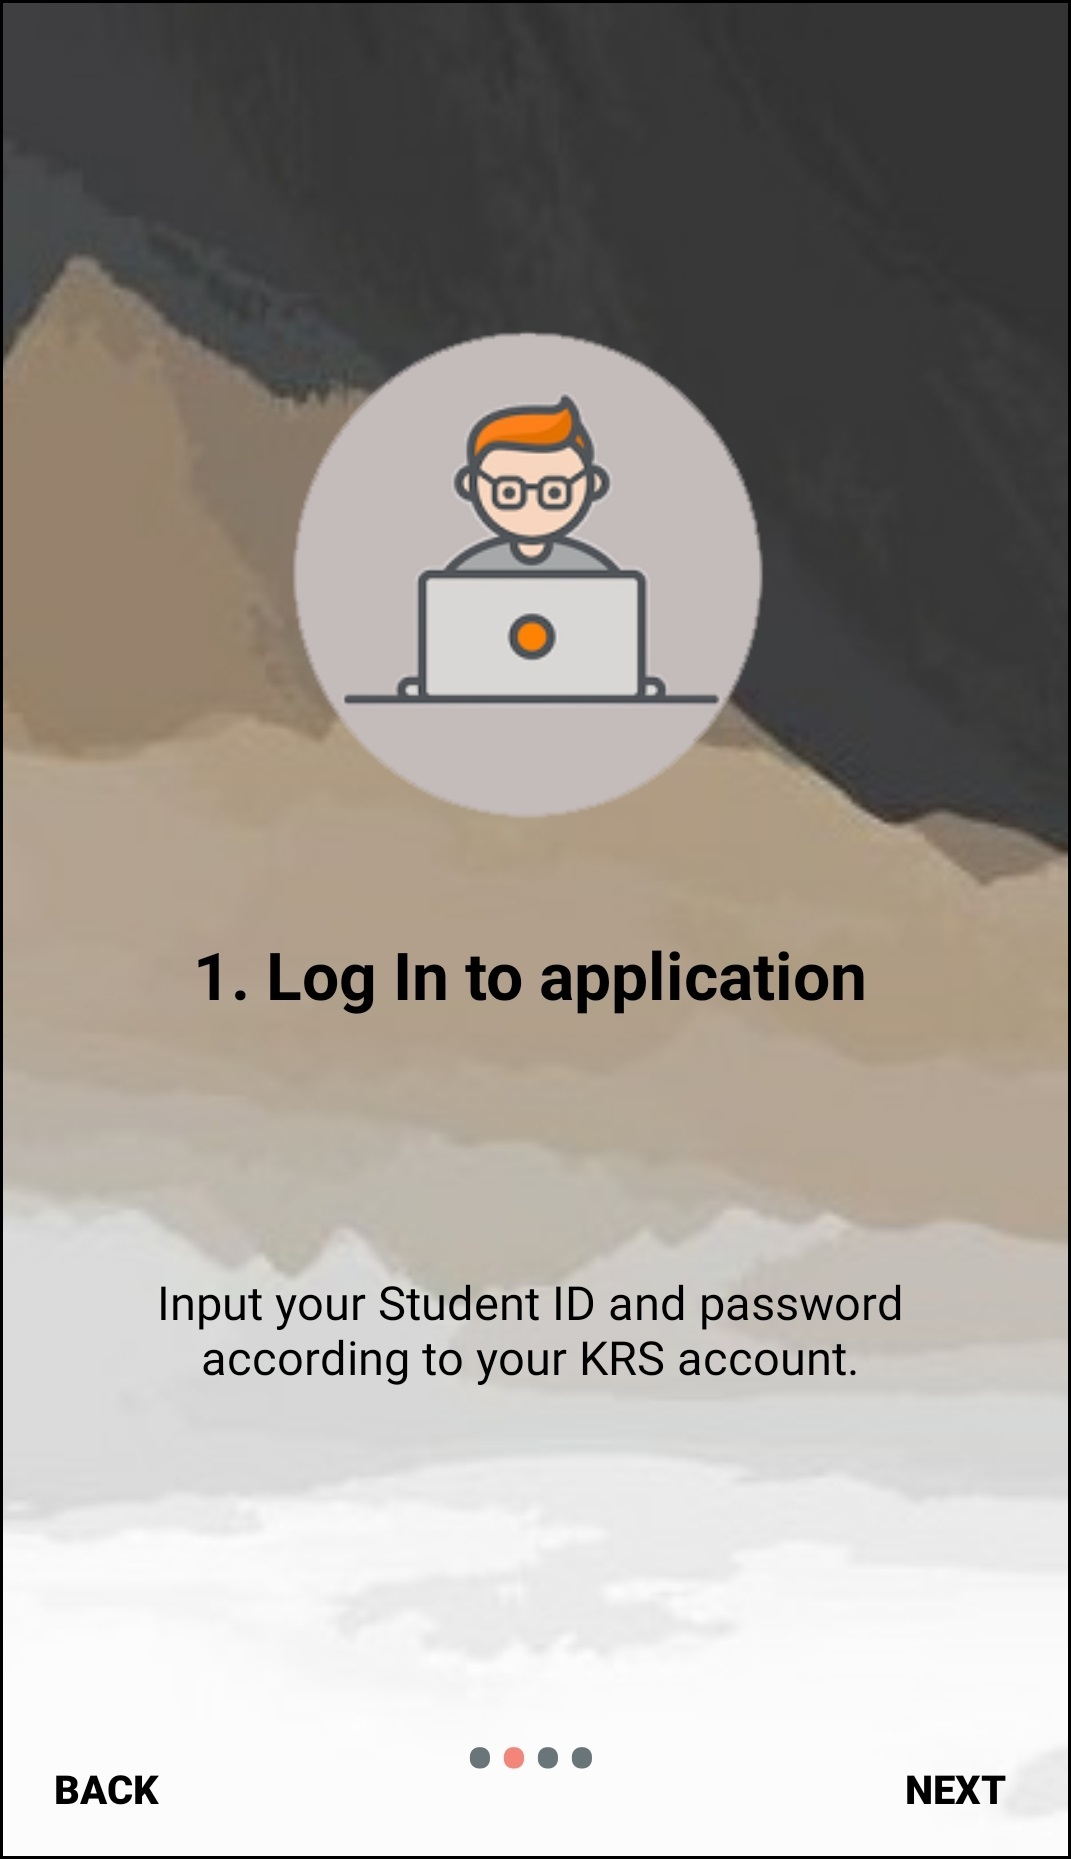
\includegraphics[width=.5\linewidth]{gambar/android/mahasiswa-1}  
  		\caption{\textit{Landing page}}
	\end{subfigure}
	\begin{subfigure}{.5\textwidth}
  		\centering
  		% include second image
  		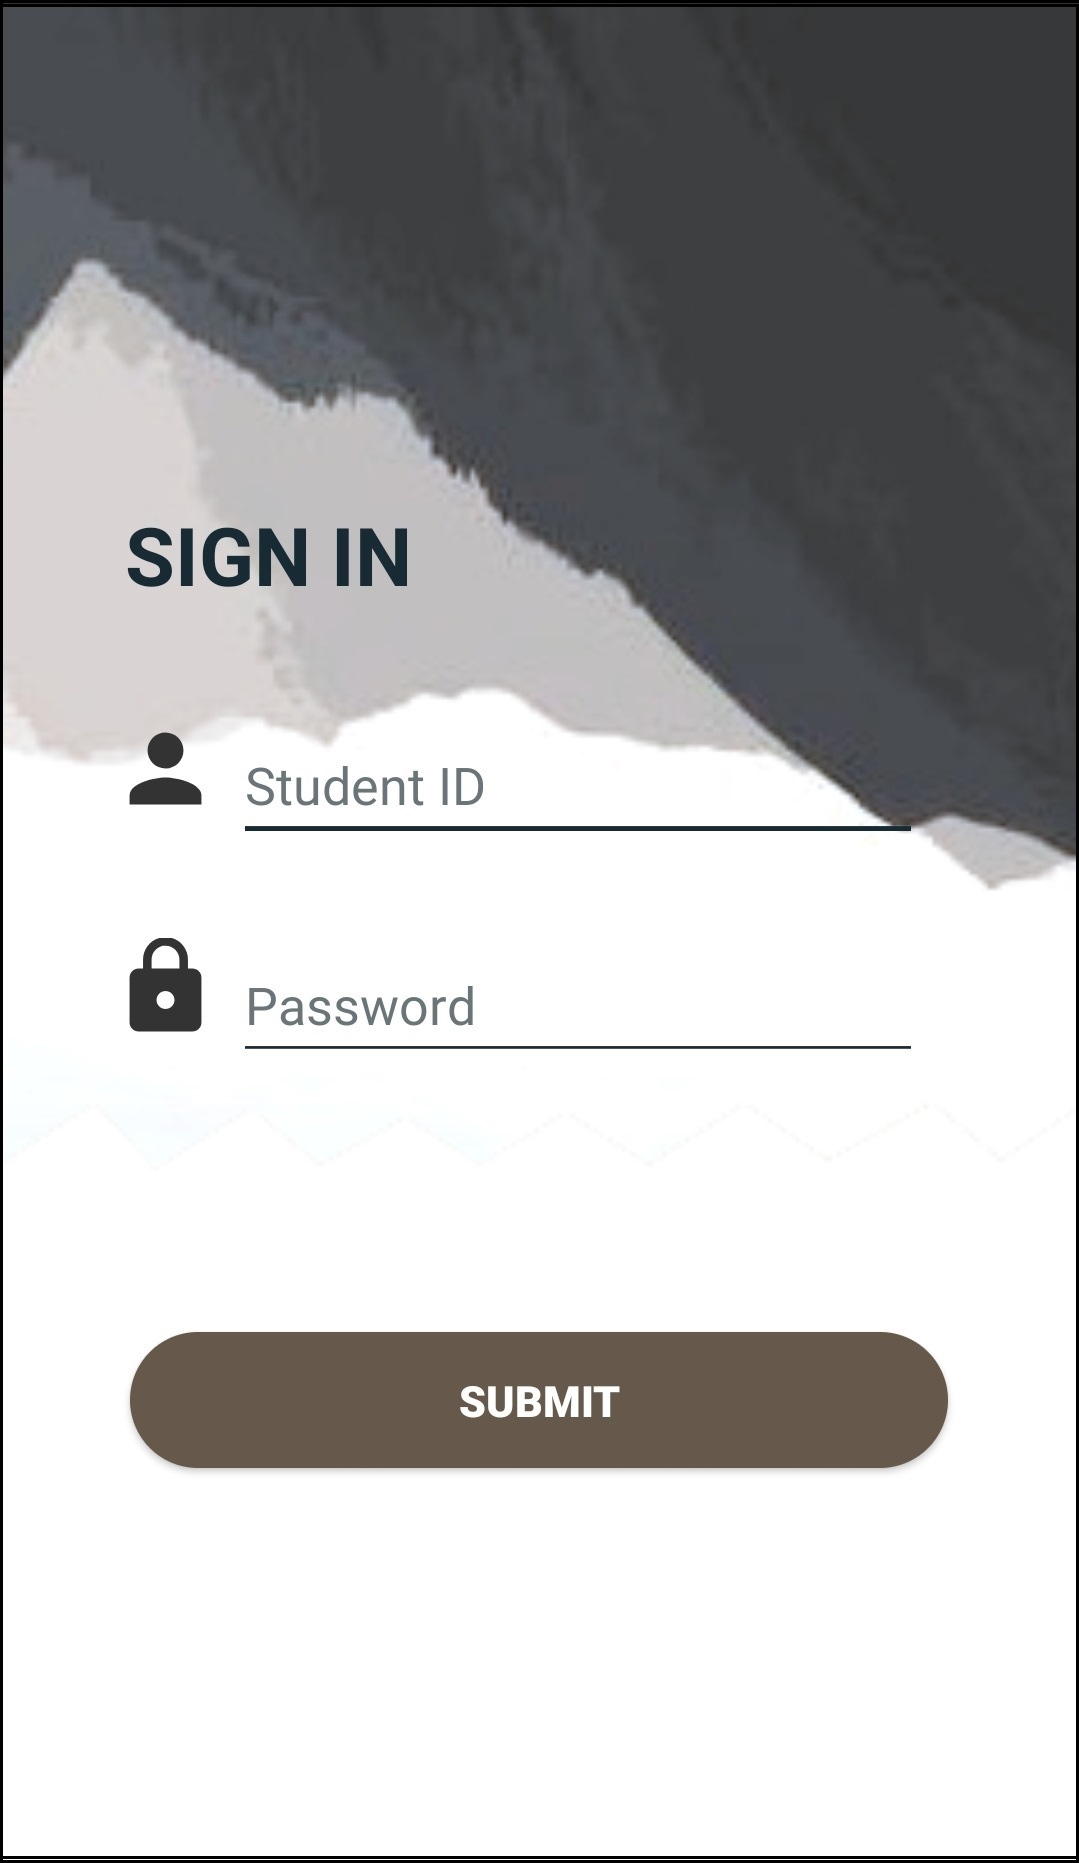
\includegraphics[width=.5\linewidth]{gambar/android/mahasiswa-2}  
  		\caption{\textit{Log in}}
	\end{subfigure}
	\vspace{1cm}
	\newline
	\begin{subfigure}{.5\textwidth}
  		\centering
  		% include third image
  		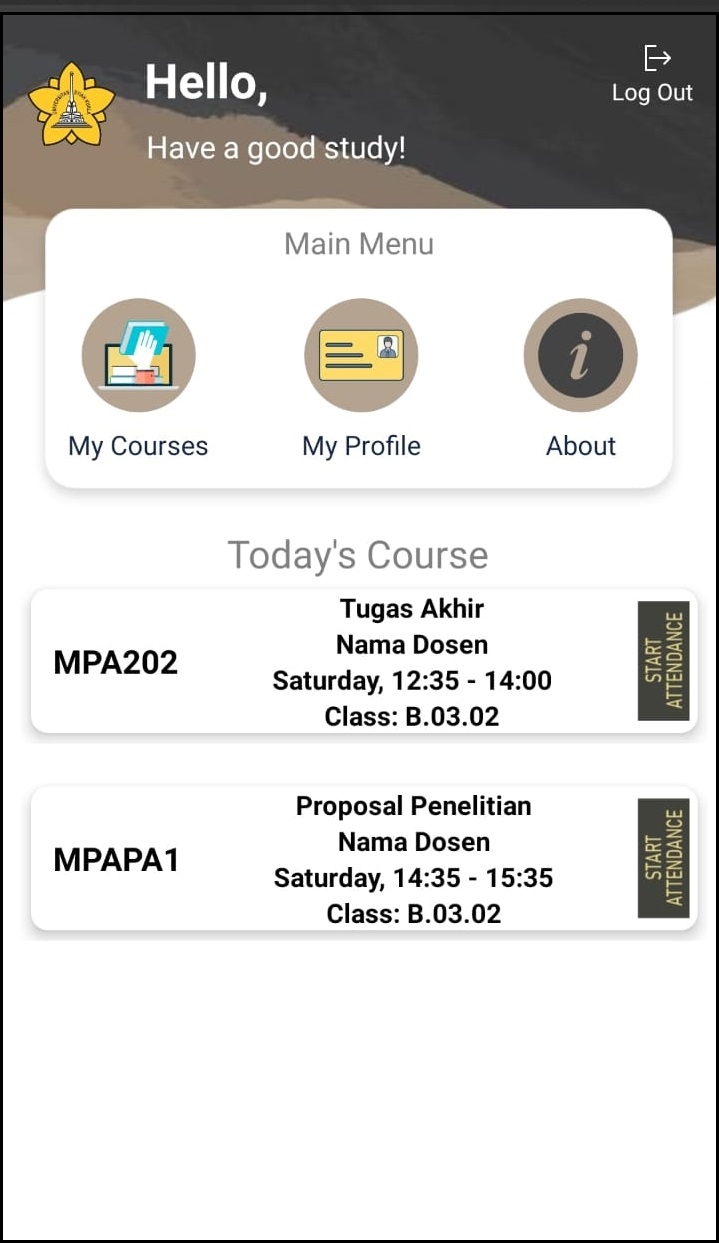
\includegraphics[width=.5\linewidth]{gambar/android/mahasiswa-3}  
  		\caption{Beranda}
	\end{subfigure}
	\begin{subfigure}{.5\textwidth}
  		\centering
  		% include fourth image
  		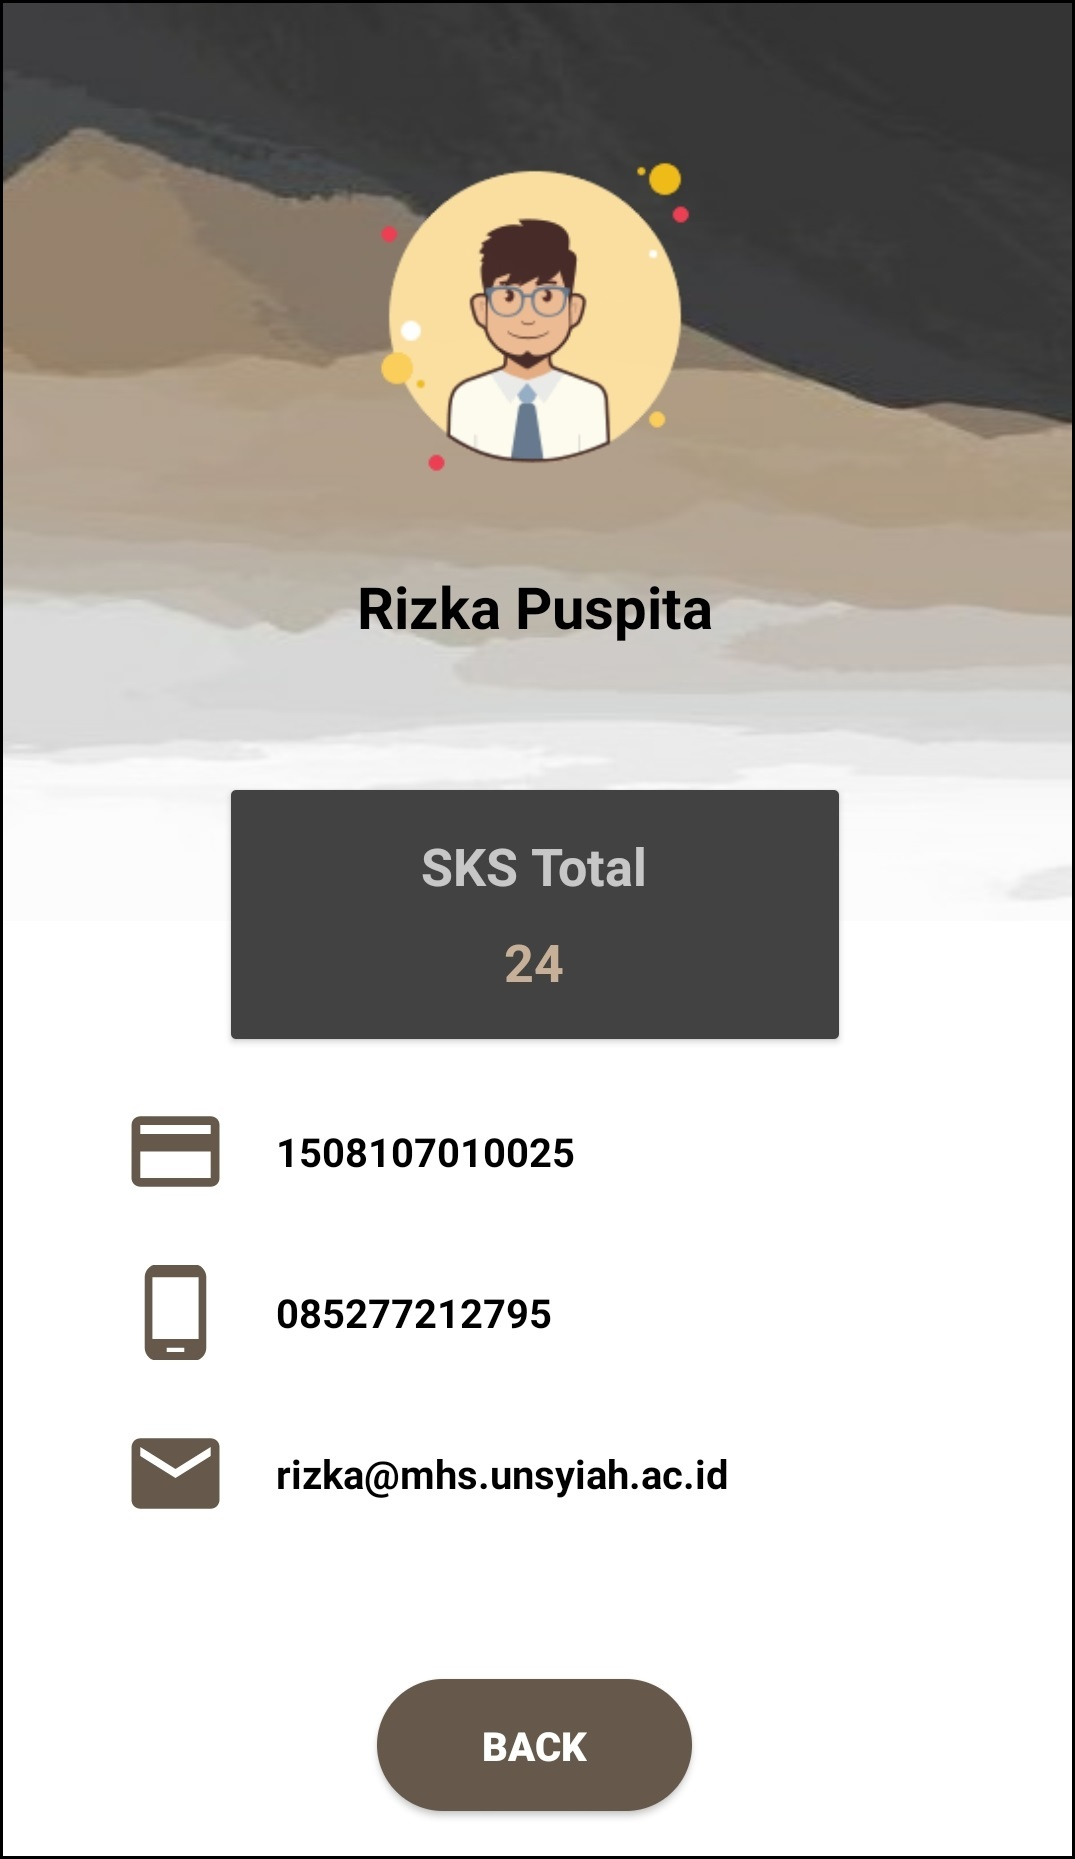
\includegraphics[width=.5\linewidth]{gambar/android/mahasiswa-4}  
  		\caption{Profil}
	\end{subfigure}
		\vspace{0.5cm}
		\caption{Tampilan Halaman Aplikasi Kehadiran Mahasiswa (Bagian 1)}
	\label{aplikasimahasiswabagian1}
	\end{figure}
	
		\par Gambar \ref{aplikasimahasiswabagian1} memperlihatkan daftar mata kuliah yang diambil oleh mahasiswa. Apabila mahasiswa menekan salah satu daftar mata kuliah, aplikasi akan memulai proses kehadiran yang dipicu oleh dosen ketika dosen telah memulai proses kehadiran. Kemudian, aplikasi akan menampilkan notifikasi untuk menghidupkan Bluetooth apabila Bluetooth pada perangkat belum hidup. Jika Bluetooth telah dihidupkan, aplikasi akan melakukan pencatatan kehadiran secara \textit{background proccess} sampai waktu matakuliah berakhir. Aplikasi akan melakukan klasifikasi dengan metode K-NN untuk memprediksi lokasi mahasiswa seperti yang terlihat pada Gambar \ref{aplikasimahasiswabagian2}.
		
	\vspace{-0cm}
	\begin{figure} [H]
	\begin{subfigure}{.5\textwidth}
  		\centering
  		% include first image
  		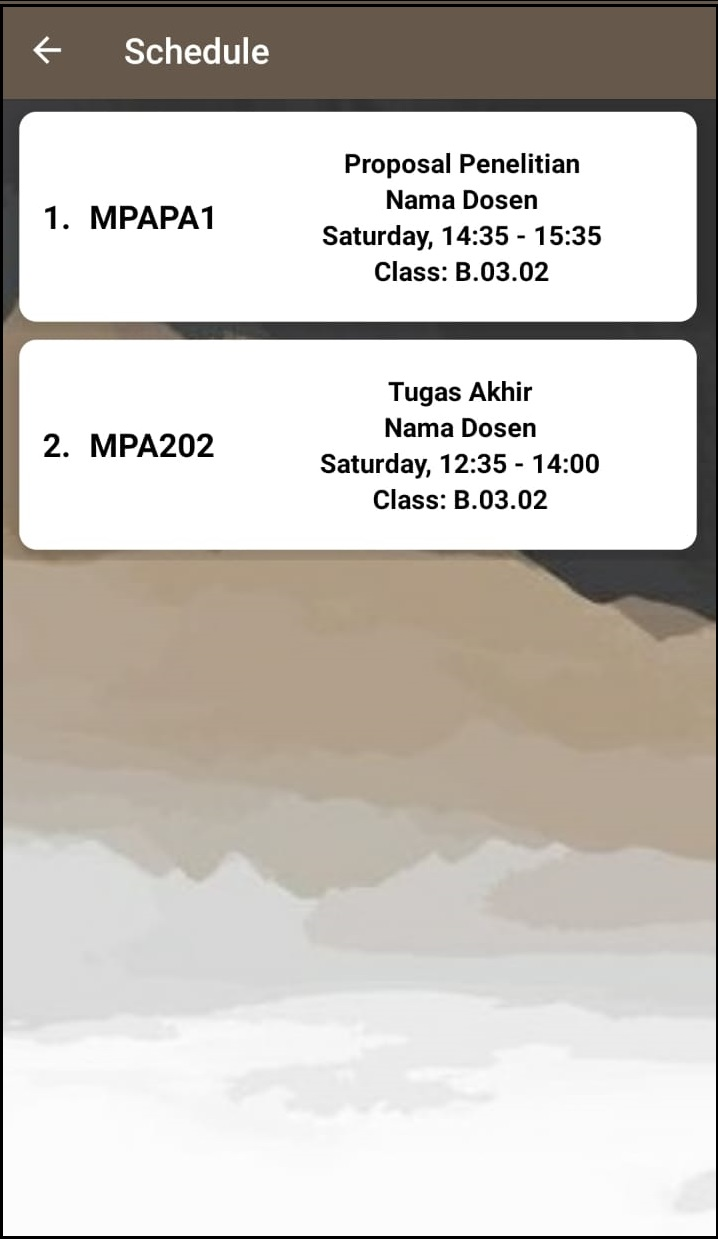
\includegraphics[width=.5\linewidth]{gambar/android/mahasiswa-5}  
  		\caption{Daftar mata kuliah}
	\end{subfigure}
	\begin{subfigure}{.5\textwidth}
  		\centering
  		% include second image
  		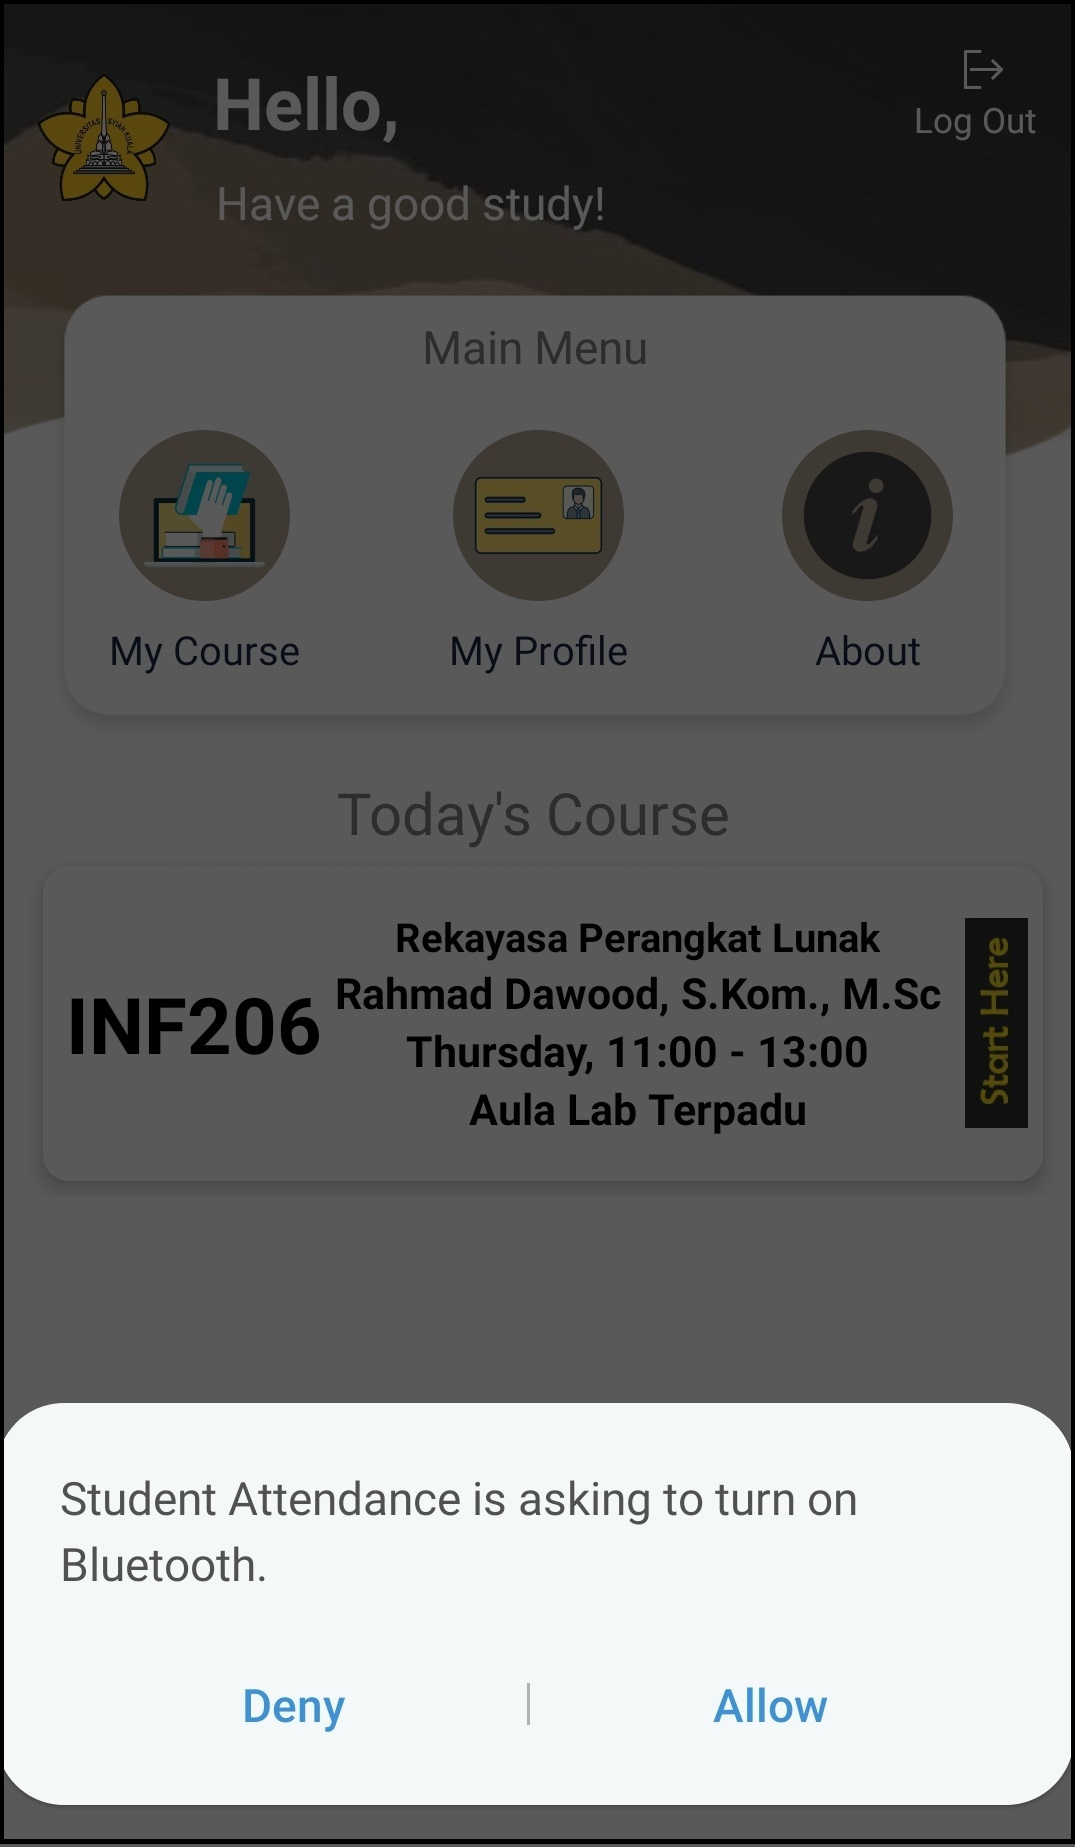
\includegraphics[width=.5\linewidth]{gambar/android/mahasiswa-6}  
  		\caption{Memulai proses kehadiran}
	\end{subfigure}
	\vspace{1cm}
	\newline
	\begin{subfigure}{.5\textwidth}
  		\centering
  		% include third image
  		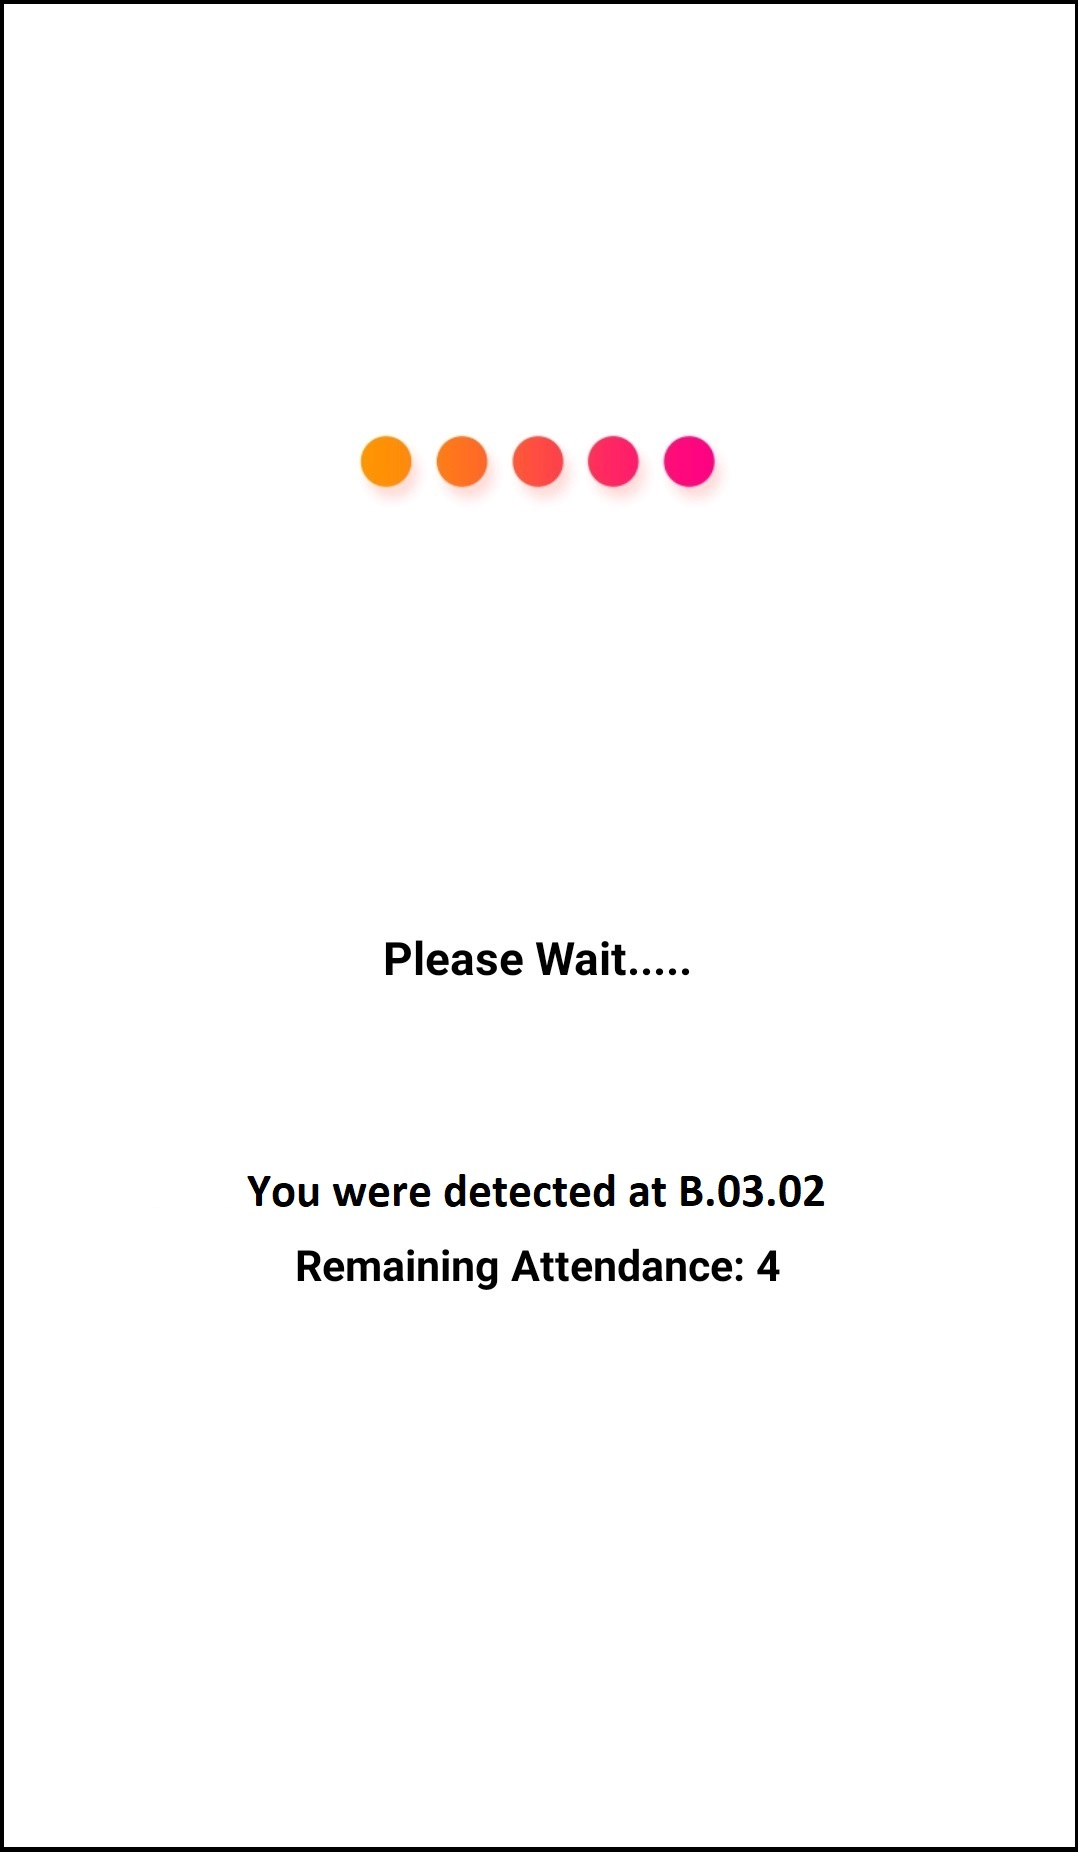
\includegraphics[width=.5\linewidth]{gambar/android/mahasiswa-7}  
  		\caption{Mahasiswa diprediksi di dalam kelas}
	\end{subfigure}
	\begin{subfigure}{.5\textwidth}
  		\centering
  		% include fourth image
  		\includegraphics[width=.5\linewidth]{gambar/android/mahasiswa-8}  
  		\caption{Mahasiswa diprediksi di luar kelas}
	\end{subfigure}
		\vspace{0.5cm}
		\caption{Tampilan Halaman Aplikasi Kehadiran Mahasiswa (Bagian 2)}
	\label{aplikasimahasiswabagian2}
	\end{figure}

	%Akhir Gambar Aplikasi Kehadiran Mahasiswa%
	
		\end{enumerate}
		
%%%%%%%%%%%%%%%%%%%%%%%%%%%%%%%%%%%%%%%%%%%akhir perancangan aplikasi mapping%%%%%%%%%%%%%%%%%%%%%%%%%%%%%%%%%%%%%%%%%%%%%%%%%%%
	\subsection{Pembuatan Sistem}
	
	\begin{enumerate}[a.]
		\item Aplikasi Mapping
		\\ Aplikasi \textit{mobile} berbasis Android yang dikembangkan menggunakan bahasa pemrograman Java dengan bantuan IDE Android Studio. Media penyimpanan basis data pada aplikasi ini menggunakan SQLite. SQLite merupakan media penyimpanan lokal untuk setiap aplikasi yang sudah terpasang di perangkat Android, dikarenakan aplikasi ini hanya perlu menyimpan data-data hasil pemindaian kekuatan sinyal Bluetooth. Aplikasi mapping ini juga sudah memiliki sertifikat Hak Kekayaan Intelektual (HKI) dengan nomor EC00201972853 yang dapat dilihat pada lampiran 1. Potongan kode program untuk melakukan pemindaian kekuatan sinyal Bluetooth dapat dilihat pada Program 4.1 berikut ini.
		\vspace{0.4cm}
			\lstset{language=Java,
			basicstyle=\ttfamily\scriptsize\color{black},
			keywordstyle=\color{javapurple}\bfseries,
			stringstyle=\color{javared},
			commentstyle=\color{javagreen},
			morecomment=[s][\color{javadocblue}]{/**}{*/},
			numbers=left,
			numberstyle=\tiny\color{black},
			showstringspaces=false,
			numbersep=10pt,
			tabsize=4,
			showspaces=false,
			showstringspaces=false,
			autogobble=true,
			xleftmargin=2em
		}
	\begin{lstlisting}[label=programScanBle]
    private HashMap<String, BTLEDevice> mBTDevicesHashMap;
    private Ble pojoBle;

    mBTDevicesHashMap = new HashMap<>(); // membuat objek kelas HashMap.
	
	/**
     * @param device parameter dari kelas BluetoothDevice yang akan ditambahkan.
     * @param rssi rssi dari kelas BluetoothDevice.
     */
    public void addDevice(BluetoothDevice device, int rssi) {
     String address = device.getAddress();
      if (!mBTDevicesHashMap.containsKey(address)) {
         if (address.equals(pojoBle.ADDRESS_1) || address.equals(pojoBle.ADDRESS_2) 
             .... 
             || address.equals(pojoBle.ADDRESS_9));
         {
             BTLEDevice btleDevice = new BTLEDevice(device);
             btleDevice.setRSSI(rssi);
             mBTDevicesHashMap.put(address, btleDevice);
             mBTDevicesArrayList.add(btleDevice);
         }
      }
      else {
            mBTDevicesHashMap.get(address).setRSSI(rssi);
        }
    }
	\end{lstlisting}
	 \captionof{lstlisting}{Potongan Kode Program Membaca Informasi Bluetooth.}

		
		\item Aplikasi Kehadiran Dosen
		\\ Aplikasi \textit{mobile} berbasis Android yang dikembangkan menggunakan bahasa pemrograman Java dengan bantuan IDE Android Studio. Media penyimpanan aplikasi ini menggunakan basis data server yaitu MySQL. Basis data server tersebut diakses melalui REST server API yang dibangun menggunakan bahasa pemrograman PHP. Aplikasi ini bertindak sebagai klien. Oleh karena itu, aplikasi ini menggunakan \textit{library} Retrofit untuk melakukan \textit{request} ke server dan menghandle \textit{response} dalam bentuk JavaScript Object Notation (JSON). Proses pengiriman data dari klien ke server dilakukan ketika dosen menekan tombol \textbf{start attendance} pada aplikasi. %Potongan kode program yang dibuat untuk melakukan pengiriman data dapat dilihat pada kode \ref{programStartAbsen} berikut ini. 
		Seorang dosen dapat terhitung menghadiri perkuliahan pada aplikasi apabila syarat-syarat di bawah ini terpenuhi:
		\begin{enumerate}[1.]
		\item Dosen menekan tombol \textbf{start attendance} 50 menit sebelum mata kuliah berakhir. 
		\item Dosen menekan tombol \textbf{start attendance} sesuai waktu yang telah ditentukan. Penentuan lokasi dilakukan dengan menggunakan metode klasifikasi K-NN yang dapat dilihat pada Program 4.2 berikut ini.
		\vspace{0.4cm}
		% KODE KNN%
	\begin{lstlisting}[label=programKNNDosen]
	public void stopScan() {
    // ambil semua nilai yang ada di HashMap (Bluetooth yang terdeteksi).
     Set<String> keys = mBTDevicesHashMap.keySet();
     String empty = "";
     String sinyal = "";
     for(String key : keys ) {
         empty += mBTDevicesHashMap.get(key).getAddress()+"\n";
         sinyal += mBTDevicesHashMap.get(key).getRSSI()+"\n";
     }
     //inisialisasi lokasi file data training.
     String train = "data_training_sequence_point.csv";
     //untuk mengambil data hasil pemindaian yg tersimpan di Hash.
     BTLE_Device ble1 = mBTDevicesHashMap.get(Ble.ADDRESS_1);
     ....  
     BTLE_Device ble9 = mBTDevicesHashMap.get(Ble.ADDRESS_9);
     //untuk kasih nilai default apabila sinyal Bluetooth tidak dapat.
     int rssi1 = ble1 == null ? -110 : ble1.getRSSI();
     ....
     int rssi9 = ble9 == null ? -110 : ble9.getRSSI();
     double[] testData = {rssi1, rssi2, ..., rssi9};
      try {
          InputStream streamTrain = getAssets().open(train);
          label = (int) KNN.knn(streamTrain, testData, 5);
          boolean masukKelas = (label == idRuang);
      } catch (IOException e) {
          e.printStackTrace();
       	}
    }
    
    \end{lstlisting}
    \captionof{lstlisting}{Potongan Kode Program Klasifikasi Metode K-NN Aplikasi Kehadiran Dosen.}

		\item Setiap mata kuliah memiliki satu sesi proses pencatatan kehadiran setiap 10 menit. Di setiap sesi tersebut, setiap aplikasi kehadiran dosen akan melakukan pencatatan kehadiran dengan pada waktu acak antara menit pertama hingga menit ke-10 setiap sesi. Sebagai contoh, mata kuliah A dimulai pada pukul 14:00 sampai pukul 16:00. Apabila satu sesi dilakukan per-10 menit sekali, maka total sesinya adalah 12 kali untuk proses pencatatan kehadiran. Misalnya sesi pertama dimulai pada pukul 14:02, pada saat itu aplikasi akan memprediksi lokasi dosen dan mengirimnya ke server untuk disesuaikan apakah kelas yang diprediksi saat itu sama dengan kelas sebenarnya. Jika prediksinya sesuai, maka dosen tersebut terhitung hadir. Kemudian, sesi kedua dimulai pada pukul 14:18. Jika prediksi yang dilakukan tidak sesuai, maka dosen tersebut terhitung tidak hadir. Proses tersebut akan berlangsung sampai sesi terakhir. Dari hasil prediksi setiap sesi tersebut, akan dihitung \textit{threshold} minimal 80\% dari jumlah proses pencatatan kehadiran yang dilakukan oleh aplikasi. 
		\end{enumerate}
		
		\vspace{0.5cm}
		\item Aplikasi Kehadiran Mahasiswa
		\\ Aplikasi \textit{mobile} berbasis Android yang dikembangkan menggunakan bahasa pemrograman Java dengan bantuan IDE Android Studio. Media penyimpanan aplikasi ini menggunakan basis data server yaitu MySQL. Basis data server tersebut diakses melalui REST server API yang dibangun menggunakan bahasa pemrograman PHP. Aplikasi ini bertindak sebagai klien. Oleh karena itu, aplikasi ini menggunakan \textit{library} Retrofit untuk melakukan \textit{request} ke server dan menghandle \textit{response} dalam bentuk JavaScript Object Notation (JSON). Proses pengiriman data dari klien ke server dilakukan ketika mahasiswa menekan tombol \textbf{start attendance} pada aplikasi. 
\newline
Seorang mahasiswa dapat terhitung menghadiri perkuliahan pada aplikasi apabila syarat-syarat di bawah ini terpenuhi:
		\begin{enumerate}[1.]
		\item Mahasiswa menekan tombol \textbf{start attendance} ketika perkuliahan sudah dimulai oleh dosen. Penentuan lokasi dilakukan dengan menggunakan metode klasifikasi K-NN yang dapat dilihat pada Program 4.3 berikut ini.
		\vspace{0.4cm}
		% KODE KNN%
	\begin{lstlisting}[label=programKNNMahasiswa]
	public void stopScan() {
    // ambil semua nilai yang ada di HashMap (Bluetooth yang terdeteksi).
     Set<String> keys = mBTDevicesHashMap.keySet();
     String empty = "";
     String sinyal = "";
     for(String key : keys ) {
         empty += mBTDevicesHashMap.get(key).getAddress()+"\n";
         sinyal += mBTDevicesHashMap.get(key).getRSSI()+"\n";
     }
     //inisialisasi lokasi file data training.
     String train = "data_training_sequence_point.csv";
     //untuk mengambil data hasil pemindaian yg tersimpan di Hash.
     BTLE_Device ble1 = mBTDevicesHashMap.get(Ble.ADDRESS_1);
     ....  
     BTLE_Device ble9 = mBTDevicesHashMap.get(Ble.ADDRESS_9);
     //untuk kasih nilai default apabila sinyal Bluetooth tidak dapat.
     int rssi1 = ble1 == null ? -110 : ble1.getRSSI();
     ....
     int rssi9 = ble9 == null ? -110 : ble9.getRSSI();
     double[] testData = {rssi1, rssi2, ..., rssi9};
      try {
          InputStream streamTrain = getAssets().open(train);
          label = (int) KNN.knn(streamTrain, testData, 5);
          boolean masukKelas = (label == idRuang);
      } catch (IOException e) {
          e.printStackTrace();
       	}
    }
    \end{lstlisting}
    \captionof{lstlisting}{Potongan Kode Program Klasifikasi Metode K-NN Aplikasi Kehadiran Mahasiswa.}
    
		\vspace{2cm}
		\item Setiap mata kuliah memiliki satu sesi proses pencatatan kehadiran setiap 10 menit. Di setiap sesi tersebut, setiap aplikasi kehadiran mahasiswa akan melakukan pencatatan kehadiran dengan pada waktu acak antara menit pertama hingga menit ke-10 setiap sesi. Sebagai contoh, mata kuliah B dimulai pada pukul 08:30 sampai pukul 10:30. Apabila satu sesi dilakukan per-10 menit sekali, maka total sesinya adalah 12 kali untuk proses pencatatan kehadiran. Misalnya sesi pertama dimulai pada pukul 08:37, pada saat itu aplikasi akan memprediksi lokasi mahasiswa dan mengirimnya ke server untuk disesuaikan apakah kelas yang diprediksi saat itu sama dengan kelas sebenarnya. Jika prediksinya sesuai, maka mahasiswa tersebut terhitung hadir. Kemudian, sesi kedua dimulai pada pukul 08:49. Jika prediksi yang dilakukan tidak sesuai, maka mahasiswa tersebut terhitung tidak hadir. Proses tersebut akan berlangsung sampai sesi terakhir. Dari hasil prediksi setiap sesi tersebut, akan dihitung \textit{threshold} minimal 80\% dari jumlah proses pencatatan kehadiran yang dilakukan oleh aplikasi.
		\end{enumerate}

	\item Aplikasi Rekap Kehadiran Dosen dan Mahasiswa Berbasis Web
	\\
	Aplikasi berbasis web ini dikembangkan dengan menggunakan bahasa pemrograman PHP dengan menggunakan prinsip MVC (Model-View-Controller). Dimana \textit{model} sebagai struktur data dan basis datanya, \textit{view} untuk menampilkan isi halaman web yang dibangun dan \textit{controller} merupakan alur bisnis sebagai jembatan \textit{model} dan \textit{view} yang menanggapi HTTP \textit{request} yang datang dari pengguna melalui \textit{browser}. Tampilan halaman \textit{log in} pada aplikasi ini dapat dilihat pada Gambar \ref{web-login}, tampilan halaman daftar kehadiran dosen dapat dilihat pada Gambar \ref{web-daftar-dosen}, tampilan halaman daftar kehadiran mahasiswa dapat dilihat pada Gambar \ref{web-daftar-mahasiswa}. Fitur utama pada aplikasi ini adalah dapat mengunduh daftar kehadiran dosen dan mahasiswa dengan format CSV untuk keperluan merekap data yang dapat dilihat pada Gambar \ref{web-csv-dosen} dan Gambar \ref{web-csv-mahasiswa}.  
	\vspace{-0.2cm}
		\begin{figure}[H]
		\center
		\includegraphics [width = 13cm, height= 6cm]{gambar/web/login}
		\caption{Halaman \textit{Log In}}
		\label{web-login}
		\end{figure}
		
		\vspace{-0.2cm}
		\begin{figure}[H]
		\center
		\includegraphics [width = 13cm, height= 6cm]{gambar/web/dashboard-dosen}
		\caption{Halaman Daftar Kehadiran Dosen}
		\label{web-daftar-dosen}
		\end{figure}
		
		\vspace{-0.2cm}
		\begin{figure}[H]
		\center
		\includegraphics [width = 13cm, height= 6cm]{gambar/web/dashboard-mahasiswa}
		\caption{Halaman Daftar Kehadiran Mahasiswa}
		\label{web-daftar-mahasiswa}
		\end{figure}
		
		\vspace{-0.2cm}
		\begin{figure}[H]
		\center
		\includegraphics [width = 11cm, height= 6.3cm]{gambar/web/rekap-dosen}
		\caption{File Unduhan CSV Rekap Kehadiran Dosen}
		\label{web-csv-dosen}
		\end{figure}
		
		\vspace{-0.2cm}
		\begin{figure}[H]
		\center
		\includegraphics [width = 11cm, height= 6.3cm]{gambar/web/rekap-mahasiswa}
		\caption{File Unduhan CSV Rekap Kehadiran Mahasiswa}
		\label{web-csv-mahasiswa}
		\end{figure}
	
	\end{enumerate}
	
	\section{\uppercase{PENGUJIAN SISTEM}}
	\par Pengujian sistem dilakukan untuk melihat apakah sistem dapat berjalan dengan tepat sesuai dengan rancangan. Beberapa pengujian yang dilakukan pada penelitian ini adalah pengujian keakuratan klasifikasi menggunakan metode klasifikasi K-NN, pengujian usabilitas dengan metode SUS dan pengujian fungsionalitas menggunakan \textit{Blackbox}. 
		
\subsection{Pengujian Keakuratan Klasifikasi Menggunakan Metode Klasifikasi K-NN}
\begin{enumerate}

\item Pengujian Keakuratan Klasifikasi Reference Point

\par Pengujian ini dianalisis menggunakan metode klasifikasi K-NN. Pengujian ini bertujuan untuk menganalisis jenis penyebaran \textit{reference point} yang terbaik dengan membandingkan \textit{F-Measure} yang didapatkan dari setiap pengujian. Data \textit{training} yang digunakan pada penelitian ini sebanyak 764 data kekuatan sinyal dengan masing-masing 324 data kekuatan sinyal untuk \textit{reference point} acak, 440 data kekuatan sinyal untuk \textit{reference point} urut dan 160 sebagai data uji. Pengumpulan data \textit{training} dilakukan dengan cara melakukan pemetaan kekuataan sinyal yang telah dijelaskan pada \textbf{BAB III}. Hasil dari proses pengujian metode klasifikasi K-NN menunjukkan bahwa dengan K=5 untuk data kekuatan sinyal \textit{reference point} urut, memiliki rata-rata \textit{F-Measure} paling baik dengan nilai 78,60\% dibandingkan dengan parameter pengujian lainnya. Hasil pengujian menggunakan metode K-NN ini  dapat dilihat pada Tabel \ref{tabelfmeasure9}.
% Please add the following required packages to your document preamble:
% \usepackage{multirow}
\begin{table}[H]
\fontsize{9}{12}\selectfont
\center
\caption{Perbandingan F-Measure}
\label{tabelfmeasure9}
\begin{tabular}{|c|c|l|c|c|c|c|}
\hline
Jenis Titik           & Nilai K            & \multicolumn{1}{c|}{Kelas Label} & Precision & Recall  & F-Measure & Rata-Rata F-Measure      \\ \hline
\multirow{3}{*}{Urut} & \multirow{3}{*}{3} & B0302                            & 90,69\%   & 66,10\% & 76,47\%   & \multirow{3}{*}{78,52\%} \\ \cline{3-6}
                      &                    & E0207                            & 82,60\%   & 70,37\% & 76,00\%    &                          \\ \cline{3-6}
                      &                    & Luar Kelas                       & 83,09\%   & 83,09\% & 83,09\%   &                          \\ \hline
\multirow{3}{*}{Urut} & \multirow{3}{*}{5} & B0302                            & 90,69\%   & 66,10\% & 76,47\%   & \multirow{3}{*}{78,60\%} \\ \cline{3-6}
                      &                    & E0207                            & 81,25\%   & 72,22\% & 76,47\%   &                          \\ \cline{3-6}
                      &                    & Luar Kelas                       & 84,05\%   & 81,69\% & 82,85\%   &                          \\ \hline
\multirow{3}{*}{Urut} & \multirow{3}{*}{7} & B0302                            & 90,69\%   & 67,24\% & 72,20\%   & \multirow{3}{*}{77,42\%} \\ \cline{3-6}
                      &                    & E0207                            & 81,63\%   & 74,07\% & 76,60\%   &                          \\ \cline{3-6}
                      &                    & Luar Kelas                       & 85,29\%   & 81,69\% & 83,45\%   &                          \\ \hline
\multirow{3}{*}{Acak} & \multirow{3}{*}{3} & B0302                            & 97,36\%   & 60,65\% & 74,74\%   & \multirow{3}{*}{77,66\%} \\ \cline{3-6}
                      &                    & E0207                            & 78,00\%   & 73,58\% & 75,72\%   &                          \\ \cline{3-6}
                      &                    & Luar Kelas                       & 81,94\%   & 83,09\% & 82,51\%   &                          \\ \hline
\multirow{3}{*}{Acak} & \multirow{3}{*}{5} & B0302                            & 97,43\%   & 59,37\% & 73,78\%   & \multirow{3}{*}{76,07\%} \\ \cline{3-6}
                      &                    & E0207                            & 75,51\%   & 71,15\% & 73,26\%   &                          \\ \cline{3-6}
                      &                    & Luar Kelas                       & 80,55\%   & 81,69\% & 81,18\%   &                          \\ \hline
\multirow{3}{*}{Acak} & \multirow{3}{*}{7} & B0302                            & 97,36\%   & 59,67\% & 74,00\%    & \multirow{3}{*}{76,89\%} \\ \cline{3-6}
                      &                    & E0207                            & 76,47\%   & 73,58\% & 74,99\%   &                          \\ \cline{3-6}
                      &                    & Luar Kelas                       & 81,69\%   & 81,69\% & 81,69\%   &                          \\ \hline
\end{tabular}
\end{table}


\par Ilustrasi dari perbandingan F-Measure setiap parameter pengujian ditampilkan pada Gambar \ref{gambar-grafik-akurasi-klasifikasi-9-beacon}.
		\begin{figure}[H]
			\center
			\shadowbox
			{\includegraphics [width = 13cm, height= 7cm]{gambar/pengujian/grafik-akurasi-klasifikasi}}
			\caption{Grafik Perbandingan F-Measure dengan Menggunakan Parameter Pengujian yang Berbeda.}
			\label{gambar-grafik-akurasi-klasifikasi-9-beacon}
		\end{figure}
		
		\vspace{2cm}
		\par Pengambilan data uji dilakukan untuk menguji tingkat keberhasilan klasifikasi dengan melihat akurasi tertinggi bergantung pada parameter nilai K yang digunakan. Pada pengujian ini terdapat titik yang sering salah diprediksi yaitu sebanyak 6 dari 6 kali pengujian. Lokasi titik yang sering salah diprediksi ditandai dengan lingkaran bewarna biru yang ditampilkan dalam bentuk ilustrasi denah yang dapat dilihat pada Gambar \ref{gambar-denah-titik-uji-b0302} dan Gambar \ref{gambar-denah-titik-uji-e0207}.
\vspace{0.2cm}
		\begin{figure}[H]
			\center
			\includegraphics [width = 11cm, height= 9cm]{gambar/denah/B0302-Uji}
			\caption{Lokasi Titik yang Sering Salah Diprediksi di Kelas B.03.02.}
			\label{gambar-denah-titik-uji-b0302}
		\end{figure}
		
		\begin{figure}[H]
			\center
			\includegraphics [width = 14cm, height= 8cm]{gambar/denah/E0207-Uji}
			\caption{Lokasi Titik yang Sering Salah Diprediksi di Kelas E.02.07.}
			\label{gambar-denah-titik-uji-e0207}
		\end{figure}
%batas batas batas batas batas batas batas batas batas batas batas batas batas

\item Pengujian Keakuratan Reference Point Berdasarkan Penggunaan Jumlah Beacon pada Ruang Kuliah B.03.02

\par Pengujian ini dianalisis menggunakan metode klasifikasi K-NN. Pengujian ini bertujuan untuk menganalisis tingkat keakuratan klasifikasi jenis \textit{reference point} terbaik yang digunakan dengan membandingkan penggunaan jumlah Beacon dengan melihat \textit{F-Measure} yang didapatkan dari setiap pengujian. Jumlah Beacon yang dibandingkan adalah 3 Beacon dan 6 Beacon. Data \textit{training} yang digunakan pada penelitian ini sebanyak 368 data kekuatan sinyal dengan masing-masing 120 data kekuatan sinyal untuk \textit{reference point} acak, 168 data kekuatan sinyal untuk \textit{reference point} urut dan 80 sebagai data uji. Pengumpulan data \textit{training} dilakukan dengan cara melakukan pemetaan kekuataan sinyal yang telah dijelaskan pada \textbf{BAB III}. Hasil dari proses pengujian metode klasifikasi K-NN menunjukkan bahwa dengan K=5 untuk data kekuatan sinyal \textit{reference point} acak menggunakan 6 Beacon, memiliki \textit{F-Measure} paling baik dengan nilai 96,20\% dibandingkan dengan parameter pengujian lainnya. Hasil pengujian menggunakan metode K-NN ini dapat dilihat secara detil pada Tabel \ref{tabelfmeasureee}.
% Please add the following required packages to your document preamble:
% \usepackage{multirow}
\begin{table}[H]
\fontsize{10}{12}\selectfont
\center
\caption{Perbandingan F-Measure}
\label{tabelfmeasureee}
\begin{tabular}{|c|c|l|c|c|c|}
\hline
Nilai K            & Jumlah BLE         & \multicolumn{1}{c|}{Jenis Titik} & Precision & Recall  & F-Measure \\ \hline
\multirow{2}{*}{3} & \multirow{2}{*}{3} & Urut                             & 67,24\%   & 97,50\% & 80,00\%    \\ \cline{3-6} 
                   &                    & Acak                             & 82,50\%   & 82,50\% & 82,50\%   \\ \hline
\multirow{2}{*}{5} & \multirow{2}{*}{3} & Urut                             & 67,24\%   & 97,50\% & 80,00\%    \\ \cline{3-6} 
                   &                    & Acak                             & 80,50\%   & 82,50\% & 81,50\%   \\ \hline
\multirow{2}{*}{7} & \multirow{2}{*}{3} & Urut                             & 67,24\%   & 97,50\% & 80,00\%    \\ \cline{3-6} 
                   &                    & Acak                             & 80,50\%   & 82,50\% & 81,50\%   \\ \hline
\multirow{2}{*}{3} & \multirow{2}{*}{6} & Urut                             & 90,70\%   & 97,50\% & 94,00\%    \\ \cline{3-6} 
                   &                    & Acak                             & 97,40\%   & 92,50\% & 95,00\%    \\ \hline
\multirow{2}{*}{5} & \multirow{2}{*}{6} & Urut                             & 90,70\%   & 97,50\% & 94,00\%    \\ \cline{3-6} 
                   &                    & Acak                             & 97,40\%   & 95,00\%  & 96,20\%   \\ \hline
\multirow{2}{*}{7} & \multirow{2}{*}{6} & Urut                             & 90,70\%   & 97,50\% & 94,00\%    \\ \cline{3-6} 
                   &                    & Acak                             & 97,40\%   & 92,50\% & 95,00\%    \\ \hline
\end{tabular}
\end{table}

\par Ilustrasi dari perbandingan F-Measure setiap parameter pengujian ditampilkan pada Gambar \ref{gambar-grafik-akurasi-klasifikasi-6-beacon}.
		\begin{figure}[H]
			\center
			\shadowbox
			{\includegraphics [width = 14cm, height= 8.7cm]{gambar/pengujian/grafik-akurasi-klasifikasi-kelas-b0302}}
			\caption{Grafik Perbandingan F-Measure dengan Menggunakan Parameter Pengujian yang Berbeda.}
			\label{gambar-grafik-akurasi-klasifikasi-6-beacon}
		\end{figure}
		
\par Berdasarkan hasil pengujian dengan parameter nilai K yang berbeda menggunakan 3 Beacon dan 6 Beacon berdasarkan jenis \textit{reference point} yang digunakan, menunjukkan bahwa penggunaan 6 Beacon mengurangi kesalahan prediksi titik dibandingkan dengan 3 Beacon. Ilustrasi perbandingan tersebut dapat ditampilkan pada Gambar \ref{gambar-grafik-titik-salah-prediksi}.	
		\begin{figure}[H]
			\center
			\shadowbox
			{\includegraphics [width = 9cm, height= 5cm]{gambar/pengujian/grafik-titik-salah-prediksi}}
			\caption{Grafik Jumlah Titik yang Salah Diprediksi.}
			\label{gambar-grafik-titik-salah-prediksi}
		\end{figure}
		

%batas batas batas batas batas batas batas batas batas batas batas batas batas	
\end{enumerate} 

\subsection{Pengujian Usabilitas Menggunakan Metode SUS}
\par Pengujian usabilitas bertujuan untuk menguji kelayakan dan kegunaan dari sistem yang akan digunakan oleh pengguna. Sebelum melakukan pengujian ini, adapun \textit{Test Plan} yang telah dibuat untuk yang dapat dilihat pada Tabel \ref{testplan-aplikasi-dosen} dan Tabel \ref{testplan-aplikasi-mahasiswa}.

\begin{table}[H]
\fontsize{10}{12}\selectfont
\center
\caption{\textit{Test Plan} Aplikasi Kehadiran Dosen}
\label{testplan-aplikasi-dosen}
\begin{tabular}{|l|l|l|l|l|}
\hline
\multicolumn{5}{|c|}{\textbf{Test Plan Aplikasi Kehadiran Dosen}}                                                                                                                                                                                                          \\ \hline
\multicolumn{5}{|l|}{\begin{tabular}[c]{@{}l@{}}Lokasi:\\ Ruang kuliah B.03.02 \\Ruang Kuliah E.03.07\end{tabular}}                                                                                                                                                                               \\ \hline
\multicolumn{5}{|l|}{\begin{tabular}[c]{@{}l@{}}Skenario:\\ 1. Dosen melakukan \textit{log in} ke aplikasi.\\ 2. Dosen memahami tampilan halaman beranda. \\ 3. Dosen melihat daftar mahasiswa yang mengambil suatu mata kuliah. \\ 4. Dosen memulai proses kehadiran.\\ 5. Dosen melihat hasil prediksi lokasi yang dilakukan oleh aplikasi.\end{tabular}} \\ \hline
\multicolumn{5}{|l|}{\begin{tabular}[c]{@{}l@{}}Alat:\\ 1. Smartphone Android\\ 2. Beacon\end{tabular}}                                                                                                                                                                    \\ \hline
\multicolumn{5}{|l|}{\begin{tabular}[c]{@{}l@{}}Hasil:\\ Hasil pengujian dapat dilihat pada tabel dan lampiran.\end{tabular}}                                                                                                                                              \\ \hline
\end{tabular}
\end{table}

\begin{table}[H]
\fontsize{10}{12}\selectfont
\center
\caption{\textit{Test Plan} Aplikasi Kehadiran Mahasiswa}
\label{testplan-aplikasi-mahasiswa}
\begin{tabular}{|l|l|l|l|l|}
\hline
\multicolumn{5}{|c|}{\textbf{Test Plan Aplikasi Kehadiran Mahasiswa}}                                                                                                                                                                                                                                                                             \\ \hline
\multicolumn{5}{|l|}{\begin{tabular}[c]{@{}l@{}}Lokasi:\\ Ruang kuliah B.03.02 \\Ruang Kuliah E.03.07\end{tabular}}                                                                                                                                                                                                                                                      \\ \hline
\multicolumn{5}{|l|}{\begin{tabular}[c]{@{}l@{}}Skenario:\\ 1. Mahasiswa melakukan \textit{log in} ke aplikasi.\\ 2. Mahasiswa melihat halaman profil data diri.\\ 3. Mahasiswa melihat daftar mata kuliah yang diambil.\\ 4. Mahasiswa memulai proses kehadiran.\\ 5. Mahasiswa melihat hasil prediksi lokasi yang dilakukan oleh aplikasi.\end{tabular}} \\ \hline
\multicolumn{5}{|l|}{\begin{tabular}[c]{@{}l@{}}Alat:\\ 1. Smartphone Android\\ 2. Beacon\end{tabular}}                                                                                                                                                                                                                                           \\ \hline
\multicolumn{5}{|l|}{\begin{tabular}[c]{@{}l@{}}Hasil:\\ Hasil pengujian dapat dilihat pada tabel dan lampiran.\end{tabular}}                                                                                                                                                                                                                     \\ \hline
\end{tabular}
\end{table}

\par Pengujian dengan metode SUS dilakukan dengan memberikan kuisioner kepada responden. Kuisioner tersebut berisi 10 pertanyaan seperti yang telah dibahas pada. Pengujian Aplikasi Kehadiran Dosen memiliki responden berjumlah 5 orang sedangkan pengujian Aplikasi Kehadiran Mahasiswa memiliki responden berjumlah 9 orang. Hasil skor pengujian metode SUS yang dilakukan dapat dilihat pada Tabel \ref{sus-aplikasi-dosen} dan Tabel \ref{sus-aplikasi-mahasiswa} berikut. 
%TABEL SUS APLIKASI DOSEN%
\begin{table}[H]
\fontsize{10}{12}\selectfont
\center
\caption{Hasil Pengujian SUS Aplikasi Kehadiran Dosen}
\label{sus-aplikasi-dosen}
\begin{tabular}{|c|c|c|c|c|c|c|c|c|c|c|c|}
\hline
\multirow{2}{*}{\textbf{Responden}} & \multicolumn{10}{c|}{\textbf{Kode Pertanyaan}}                                                                                                                  & \multirow{2}{*}{\textbf{Skor SUS}} \\ \cline{2-11}
                                    & \textbf{R1} & \textbf{R2} & \textbf{R3} & \textbf{R4} & \textbf{R5} & \textbf{R6} & \textbf{R7} & \textbf{R8} & \textbf{R9} & \multicolumn{1}{l|}{\textbf{R10}} &                                    \\ \hline
1                                   & 3           & 2           & 4           & 1           & 4           & 4           & 4           & 3           & 4           & 2                                 & 67,5                               \\ \hline
2                                   & 5           & 2           & 5           & 4           & 4           & 2           & 4           & 2           & 4           & 5                                 & 67,5                               \\ \hline
3                                   & 4           & 2           & 4           & 1           & 4           & 2           & 4           & 1           & 4           & 4                                 & 75,0                                 \\ \hline
4                                   & 5           & 1           & 5           & 2           & 5           & 2           & 5           & 1           & 5           & 1                                 & 95,0                                 \\ \hline
5                                   & 5           & 2           & 5           & 1           & 4           & 2           & 5           & 2           & 5           & 2                                 & 87,5                               \\ \hline
\multicolumn{11}{|c|}{\textbf{Rata - Rata}}                                                                                                                                                           & \textbf{78,5}                      \\ \hline
\end{tabular}
\end{table}

%TABEL SUS APLIKASI MAHASISWA%
\begin{table}[H]
\fontsize{10}{12}\selectfont
\center
\caption{Hasil Pengujian SUS Aplikasi Kehadiran Mahasiswa}
\label{sus-aplikasi-mahasiswa}
\begin{tabular}{|c|c|c|c|c|c|c|c|c|c|c|c|}
\hline
\multirow{2}{*}{\textbf{Responden}} & \multicolumn{10}{c|}{\textbf{Kode Pertanyaan}}                                                                                                                  & \multirow{2}{*}{\textbf{Skor SUS}} \\ \cline{2-11}
                                    & \textbf{R1} & \textbf{R2} & \textbf{R3} & \textbf{R4} & \textbf{R5} & \textbf{R6} & \textbf{R7} & \textbf{R8} & \textbf{R9} & \multicolumn{1}{l|}{\textbf{R10}} &                                    \\ \hline
1                                   & 5           & 1           & 4           & 1           & 4           & 1           & 5           & 1           & 5           & 1                                 & 95,0                                 \\ \hline
2                                   & 5           & 2           & 4           & 2           & 4           & 2           & 4           & 2           & 2           & 2                                 & 72,5                               \\ \hline
3                                   & 5           & 2           & 5           & 2           & 5           & 1           & 5           & 1           & 5           & 2                                 & 92,5                               \\ \hline
4                                   & 5           & 1           & 5           & 1           & 5           & 1           & 5           & 1           & 5           & 1                                 & 100,0                                \\ \hline
5                                   & 5           & 1           & 5           & 2           & 5           & 1           & 5           & 1           & 5           & 2                                 & 95,0                                 \\ \hline
6                                   & 5           & 2           & 4           & 1           & 4           & 2           & 4           & 1           & 5           & 2                                 & 85,0                                 \\ \hline
7                                   & 5           & 3           & 4           & 2           & 4           & 2           & 4           & 2           & 3           & 5                                 & 65,0                                 \\ \hline
8                                   & 4           & 1           & 5           & 2           & 4           & 2           & 4           & 1           & 5           & 4                                 & 80,0                                 \\ \hline
9                                   & 5           & 1           & 5           & 2           & 5           & 2           & 5           & 2           & 5           & 2                                 & 90,0                                 \\ \hline
\multicolumn{11}{|c|}{\textbf{Rata - Rata}}                                                                                                                                                             & \textbf{86,1}                      \\ \hline
\end{tabular}
\end{table}

\par Berdasarkan hasil pengujian SUS yang telah dilakukan diatas, hasil rata-rata pengujian Aplikasi Kehadiran Dosen mendapatkan skor sebesar 78,5\% sedangkan hasil rata-rata pengujian Aplikasi Kehadiran Mahasiswa mendapatkan skor sebesar 86,1\%. Dapat dilihat bahwa kedua aplikasi yang telah dibangun memiliki skor interpretasi \textbf{"dapat diterima"} berdasarkan Tabel 3.4.  

\subsection{Pengujian Fungsionalitas Menggunakan Blackbox}
\par Pengujian \textit{Blackbox} dilakukan dengan tujuan untuk menguji fungsionalitas dari aplikasi dengan menjalankan aplikasi tersebut apakah sesuai dengan alur bisnis yang diinginkan. Pengujian ini melihat fungsi yang tidak sesuai pada aplikasi dan kesalahan-kesalahan aplikasi dalam mengerjakan suatu perintah. Pengujian ini dilakukan pada Aplikasi Mapping, Aplikasi Kehadiran Dosen, Aplikasi Kehadiran Mahasiswa, dan Aplikasi Web Rekap Kehadiran Dosen dan Mahasiswa. Beberapa fitur aplikasi yang diuji menggunakan \textit{Blackbox Testing} dapat dilihat pada Tabel \ref{blackbox-aplikasi-mapping}, Tabel \ref{blackbox-aplikasi-dosen}, Tabel \ref{blackbox-aplikasi-mahasiswa}, dan Tabel \ref{blackbox-web-admin}.
%TABEL APLIKASI MAPPING%
\begin{table}[H]
\fontsize{10}{12}\selectfont
\center
\caption{Pengujian \textit{Blackbox} Aplikasi Mapping}
\label{blackbox-aplikasi-mapping}
\begin{tabular}{|c|l|l|l|c|}
\hline
\textbf{No.} & \multicolumn{1}{c|}{\textbf{Nama Pengujian}}                                       & \multicolumn{1}{c|}{\textbf{Skenario}}                                                                                        & \multicolumn{1}{c|}{\textbf{Tampilan}}                                                                    & \textbf{Hasil}                \\ \hline
1.           & \begin{tabular}[c]{@{}l@{}}Menghidupkan \\ Bluetooth\end{tabular}                  & \begin{tabular}[c]{@{}l@{}}Klik tombol \textbf{Allow} \\ pada notifikasi yang\\ muncul\end{tabular}                                  & \begin{tabular}[c]{@{}l@{}}Bluetooth akan \\ hidup\end{tabular}                                           & Berhasil                      \\ \hline
2.           & \begin{tabular}[c]{@{}l@{}}Lakukan proses \\ pemindaian \\ sinyal BLE\end{tabular} & Klik tombol \textbf{"Scan"}                                                                                                            & \begin{tabular}[c]{@{}l@{}}Muncul nama BLE, \\ MAC Address BLE \\ dan kekuatan sinyal \\ BLE\end{tabular} & Berhasil                      \\ \hline
3.           & \begin{tabular}[c]{@{}l@{}}Menyimpan data \\ ke tabel titik acak\end{tabular}      & \begin{tabular}[c]{@{}l@{}}Mengisi nama ruang \\ kemudian klik tombol \\ \textbf{Save to} dan pilih \\ tabel titik acak\end{tabular} & \begin{tabular}[c]{@{}l@{}}Muncul \textit{pop up} \\ untuk memilih \\ tabel\end{tabular}                           & Berhasil                      \\ \hline
4.           & \begin{tabular}[c]{@{}l@{}}Menyimpan data \\ ke tabel titik urut\end{tabular}      & \begin{tabular}[c]{@{}l@{}}Mengisi nama ruang \\ kemudian klik tombol \\ \textbf{Save to} dan pilih \\ tabel titik urut\end{tabular} & \begin{tabular}[c]{@{}l@{}}Muncul \textit{pop up} \\ untuk memilih \\ tabel\end{tabular}                           & Berhasil                      \\ \hline
5.           & \begin{tabular}[c]{@{}l@{}}Melihat data \\ yang tersimpan\end{tabular}             & \begin{tabular}[c]{@{}l@{}}Klik tombol \\ \textbf{Show Data}\end{tabular}                                                            & \begin{tabular}[c]{@{}l@{}}Diarahkan ke \\ halaman daftar \\ data yang tersimpan\end{tabular}             & Berhasil                      \\ \hline
6.           & \begin{tabular}[c]{@{}l@{}}Menghapus data \\ yang tersimpan\end{tabular}           & \begin{tabular}[c]{@{}l@{}}Klik icon \textbf{Tong} \\ \textbf{Sampah}\end{tabular}                                                              & \begin{tabular}[c]{@{}l@{}}Muncul notifikasi \\ dan konfirmasi \\ untuk menghapus \\ data\end{tabular}    & \multicolumn{1}{l|}{Berhasil} \\ \hline
\end{tabular}
\end{table}

%BLACKBOX APLIKASI DOSEN%
\begin{table}[H]
\fontsize{10}{12}\selectfont
\center
\caption{Pengujian \textit{Blackbox } Aplikasi Kehadiran Dosen}
\label{blackbox-aplikasi-dosen}
\begin{tabular}{|c|l|l|l|c|}
\hline
No. & \multicolumn{1}{c|}{\textbf{Nama Pengujian}}                                                                              & \multicolumn{1}{c|}{\textbf{Skenario}}                                                                                    & \multicolumn{1}{c|}{\textbf{Tampilan}}                                                                                  & Hasil    \\ \hline
1.  & \begin{tabular}[c]{@{}l@{}}Melakukan \textit{log in} \\ ke aplikasi\end{tabular}                                          & \begin{tabular}[c]{@{}l@{}}Klik tombol \textbf{Submit} \\ setelah selesai \\ mengisi form \textit{log in}\end{tabular}             & \begin{tabular}[c]{@{}l@{}}Diarahkan ke \\ halaman beranda \\ aplikasi apabila \\ berhasil \textit{log in}\end{tabular} & Berhasil \\ \hline
2.  & \begin{tabular}[c]{@{}l@{}}Melihat informasi \\ suatu mata kuliah\end{tabular}                                   & \begin{tabular}[c]{@{}l@{}}Klik salah satu daftar \\ mata kuliah\end{tabular}                                    & \begin{tabular}[c]{@{}l@{}}Diarahkan ke \\ halaman informasi \\ mata kuliah\end{tabular}                       & Berhasil \\ \hline
3.  & \begin{tabular}[c]{@{}l@{}}Menghidupkan \\ Bluetooth\end{tabular}                                                & \begin{tabular}[c]{@{}l@{}}Klik tombol \textbf{Allow} \\ pada notifikasi yang \\ muncul\end{tabular}                      & \begin{tabular}[c]{@{}l@{}}Bluetooth akan \\ menyala\end{tabular}                                              & Berhasil \\ \hline
4.  & \begin{tabular}[c]{@{}l@{}}Melihat daftar \\ nama mahasiswa \\ yang mengambil  \\ suatu mata kuliah\end{tabular} & \begin{tabular}[c]{@{}l@{}}Klik tombol \\ \textbf{Show Students} pada \\ halaman informasi \\ mata kuliah\end{tabular}    & \begin{tabular}[c]{@{}l@{}}Diarahkan ke \\ halaman daftar \\ nama mahasiswa\end{tabular}                       & Berhasil \\ \hline
5.  & \begin{tabular}[c]{@{}l@{}}Memulai proses \\ kehadiran\end{tabular}                                              & \begin{tabular}[c]{@{}l@{}}Klik tombol \\ \textbf{Start Attendance} \\ pada halaman \\ informasi mata kuliah\end{tabular} & \begin{tabular}[c]{@{}l@{}}Secara \textit{background} \\ \textit{proccess} aplikasi \\ akan memproses \\ kehadiran\end{tabular}  & Berhasil \\ \hline
\end{tabular}
\end{table}

%BLACKBOX APLIKASI MAHASISWA%
\begin{table}[H]
\fontsize{10}{12}\selectfont
\center
\caption{Pengujian \textit{Blackbox} Aplikasi Kehadiran Mahasiswa}
\label{blackbox-aplikasi-mahasiswa}
\begin{tabular}{|c|l|l|l|c|}
\hline
No. & \multicolumn{1}{c|}{\textbf{Nama Pengujian}}                                                   & \multicolumn{1}{c|}{\textbf{Skenario}}                                                                                    & \multicolumn{1}{c|}{\textbf{Tampilan}}                                                                                  & Hasil                         \\ \hline
1.  & \begin{tabular}[c]{@{}l@{}}Melakukan \textit{log in}\\ ke aplikasi\end{tabular}                & \begin{tabular}[c]{@{}l@{}}Klik tombol \textbf{Submit} \\ setelah selesai \\ mengisi form \textit{log in}\end{tabular}             & \begin{tabular}[c]{@{}l@{}}Diarahkan ke \\ halaman beranda \\ aplikasi apabila \\ berhasil \textit{log in}\end{tabular} & Berhasil                      \\ \hline
2.  & \begin{tabular}[c]{@{}l@{}}Melihat daftar \\ mata kuliah \\ yang diambil\end{tabular} & Klik icon \textbf{My Course}                                                                                              & \begin{tabular}[c]{@{}l@{}}Diarahkan ke \\ halaman daftar \\ mata kuliah\end{tabular}                          & Berhasil                      \\ \hline
3.  & \begin{tabular}[c]{@{}l@{}}Melihat profil \\ data diri\end{tabular}                   & Klik icon \textbf{My Profile                                                                                            } & \begin{tabular}[c]{@{}l@{}}Diarahkan ke \\ halaman profil\end{tabular}                                         & \multicolumn{1}{l|}{Berhasil} \\ \hline
4.  & \begin{tabular}[c]{@{}l@{}}Menghidupkan \\ Bluetooth\end{tabular}                     & \begin{tabular}[c]{@{}l@{}}Klik tombol \textbf{Allow} \\ pada notifikasi \\ yang muncul\end{tabular}                      & \begin{tabular}[c]{@{}l@{}}Bluetooth akan \\ menyala\end{tabular}                                              & Berhasil                      \\ \hline
5.  & \begin{tabular}[c]{@{}l@{}}Memulai \\ proses kehadiran\end{tabular}                   & \begin{tabular}[c]{@{}l@{}}Klik tombol \\ \textbf{Start Attendance} \\ pada salah satu \\ daftar mata kuliah\end{tabular} & \begin{tabular}[c]{@{}l@{}}Secara \textit{background} \\ \textit{proccess} aplikasi \\ akan memproses \\ kehadiran\end{tabular}  & Berhasil                      \\ \hline
\end{tabular}
\end{table}

%BLACKBOX WEB ADMIN%
\begin{table}[H]
\fontsize{10}{12}\selectfont
\center
\caption{Pengujian \textit{Blackbox} Aplikasi Web Rekap Kehadiran Dosen dan Mahasiswa}
\label{blackbox-web-admin}
\begin{tabular}{|c|l|l|l|c|}
\hline
No. & \multicolumn{1}{c|}{\textbf{Nama Pengujian}}                                                   & \multicolumn{1}{c|}{\textbf{Skenario}}                                                                                    & \multicolumn{1}{c|}{\textbf{Tampilan}}                                                                                  & Hasil                         \\ \hline
1.  & \begin{tabular}[c]{@{}l@{}}Melakukan \textit{log in}\\ ke aplikasi\end{tabular}                & \begin{tabular}[c]{@{}l@{}}Klik tombol \\ \textbf{Submit} setelah \\ selesai mengisi \\ form \textit{log in}\end{tabular}          & \begin{tabular}[c]{@{}l@{}}Diarahkan ke \\ halaman beranda \\ aplikasi apabila \\ berhasil \textit{log in}\end{tabular} & Berhasil                      \\ \hline
2.  & \begin{tabular}[c]{@{}l@{}}Melihat daftar \\ mata kuliah \\ yang diambil\end{tabular} & \begin{tabular}[c]{@{}l@{}}Klik icon \\ \textbf{My Course}\end{tabular}                                                   & \begin{tabular}[c]{@{}l@{}}Diarahkan ke \\ halaman daftar \\ mata kuliah\end{tabular}                          & Berhasil                      \\ \hline
3.  & \begin{tabular}[c]{@{}l@{}}Melihat profil \\ data diri\end{tabular}                   & \begin{tabular}[c]{@{}l@{}}Klik icon \\ \textbf{My Profile}\end{tabular}                                                  & \begin{tabular}[c]{@{}l@{}}Diarahkan ke \\ halaman profil\end{tabular}                                         & \multicolumn{1}{l|}{Berhasil} \\ \hline
4.  & \begin{tabular}[c]{@{}l@{}}Menghidupkan \\ Bluetooth\end{tabular}                     & \begin{tabular}[c]{@{}l@{}}Klik tombol \\ \textbf{Allow} pada \\ notifikasi yang\\ muncul\end{tabular}                    & \begin{tabular}[c]{@{}l@{}}Bluetooth akan \\ menyala\end{tabular}                                              & Berhasil                      \\ \hline
5.  & \begin{tabular}[c]{@{}l@{}}Memulai \\ proses kehadiran\end{tabular}                   & \begin{tabular}[c]{@{}l@{}}Klik tombol \\ \textbf{Start Attendance} \\ pada salah satu \\ daftar mata kuliah\end{tabular} & \begin{tabular}[c]{@{}l@{}}Secara \textit{background} \\ \textit{proccess} aplikasi \\ akan memproses \\ kehadiran\end{tabular}  & Berhasil                      \\ \hline
\end{tabular}
\end{table}

%AKHIR DARI TABEL%
\par Berdasarkan hasil \textit{Blackbox Testing} dari tabel diatas menunjukkan bahwa Aplikasi Mapping, Aplikasi Kehadiran Dosen, Aplikasi Kehadiran Mahasiswa, dan Aplikasi Web Rekap Kehadiran Dosen dan Mahasiswa dapat berjalan dengan baik dibuktikan dengan  \textbf{"berhasil"} pada kolom hasil pengujian masing-masing fitur yang dikerjakan.


\begin{comment}
\bibliography{daftar-pustaka}
\end{comment}

  %-------------------------------------------------------------------------------
%                            	BAB V
%               		KESIMPULAN DAN SARAN
%-------------------------------------------------------------------------------
\fancyhf{}
\fancyfoot[C]{\thepage}
\chapter{KESIMPULAN DAN SARAN}

\section{\uppercase{KESIMPULAN}}
Berdasarkan penelitian yang telah dilakukan, dapat diambil kesimpulan bahwa:
\begin{enumerate}
	\item Cara kerja layanan \textit{Crowdsourcing Indoor Localization System} berbasis BLE untuk proses penentuan lokasi dan estimasi orang di dalam gedung menggunakan aplikasi berbasis Android telah berhasil diimplementasikan dengan memanfaatkan algoritma klasifikasi SVM.
	\item Metode klasifikasi SVM untuk data kekuatan sinyal pada jenis \textit{reference point} urut telah berhasil diimplementasikan dengan memiliki rata-rata \textit{F-Measure} dengan nilai 95\%.
	\item Hasil analisis keakuratan algoritma SVM di setiap lokasi di dalam gedung A FMIPA USK yang diuji coba sebanyak 20 kali tiap label menunjukkan hasil keakuratan sebesar 92,5\%.
	\item Hasil pengujian fungsionalitas menggunakan metode Black Box menghasilkan semua fitur berhasil dijalankan dengan baik. Kemudian pengujian usability menggunakan metode UMUX mendapat nilai 93,84 sedangkan skor UMUX-lite adalah 84,13. Kedua skor tersebut berada pada kategori A+. Hal ini bermakna aplikasi dapat diterima dengan baik, dan memiliki skala B atau \textit{Excellence} berdasarkan grafik pada gambar \ref{grafikumuxlite}.
\end{enumerate}



\section{\uppercase{SARAN}}

Penelitian ini masih banyak kekurangan sehingga perlu dikembangkan agar menjadi lebih baik. Berikut adalah saran untuk penelitian ini:
\begin{enumerate}
	\item Aplikasi ini sebaiknya dikembangkan lebih luas lagi untuk seluruh area gedung kampus hingga satu Universitas agar pemanfaatan aplikasi bisa lebih luas lagi.
	\item Aplikasi LocaLization sebaiknya dibangun juga  versi iOS.
	\item Mencari metode klasifikasi yang lebih baik lagi untuk memprediksi lokasi pengguna.
	\item Sebaiknya ditambahkan lagi jumlah Beacon di setiap ruangan supaya meningkatkan keakuratan klasifikasi.

\end{enumerate}

\fancyhf{}
\fancyfoot[R]{\thepage}
\begin{comment}
\bibliography{daftar-pustaka}
\end{comment}


  \begin{spacing}{1}
    \bibliography{daftar-pustaka}
  \end{spacing}
  \addcontentsline{toc}{chapter}{DAFTAR KEPUSTAKAAN}
  %-----------------------------------------------------------------
  % Disini akhir masukan Daftar Pustaka
  %-----------------------------------------------------------------

  %
% @author Kurnia Saputra
% @version 1.0
% 
% Hanya sebuah pembatas bertuliskan LAMPIRAN ditengah halaman. 
% 

\begin{titlepage}
	\centering 
	\vspace*{6cm}
	\noindent \Huge{LAMPIRAN}
	%\addChapter{LAMPIRAN}
	\addcontentsline{toc}{chapter}{LAMPIRAN}
\end{titlepage}
  %-----------------------------------------------------------------------------%
% \addcontentsline{toc}{chapter}{LAMPIRAN 1}
% \chapter*{Lampiran 1}
% \newappendix{Lampiran 1. Sertifikat HKI Aplikasi Mapping}
% \begin{figure}[H]
%   \centering
%   \includegraphics[width = 14cm, height = 21cm]{gambar/lampiran/sertifikat}
% \end{figure}

%------------------------------------------------------%
\addcontentsline{toc}{chapter}{LAMPIRAN 1}
\chapter*{Lampiran 1}
\newappendix{Lampiran 1. Foto Dokumentasi Proses \textit{Mapping}}
\begin{figure}[H]
  \center
  \includegraphics [width = 13.5 cm, height= 6.75 cm]{gambar/lampiran/lamp1a.jpg}
\end{figure}
\begin{figure}[H]
  \center
  \includegraphics [width = 13.5 cm, height= 6.75 cm]{gambar/lampiran/lamp1d.jpg}
\end{figure}
\begin{figure}[H]
  \center
  \includegraphics [width = 13.5 cm, height= 6.75 cm]{gambar/lampiran/lamp1b.JPG}
\end{figure}
\label{sus-dosen}



\vspace{2cm}




%-----------------------------------------------------------------------------%
\addcontentsline{toc}{chapter}{LAMPIRAN 2}
\chapter*{Lampiran 2}
\newappendix{Lampiran 2. Foto Dokumentasi Proses Pengujian  \textit{Usability} dan Fungsionalitas}

\begin{figure}[H]
  \center
  \includegraphics [width = 13.5 cm, height= 6.75 cm]{gambar/lampiran/umux1.jpeg}
\end{figure}
\begin{figure}[H]
  \center
  \includegraphics [width = 13.5 cm, height= 6.75 cm]{gambar/lampiran/umux5.jpeg}
\end{figure}
\begin{figure}[H]
  \center
  \includegraphics [width = 13.5 cm, height= 6.75 cm]{gambar/lampiran/umux3.jpeg}
\end{figure}
\label{sus-dosen}
\begin{figure}[H]
  \center
  \includegraphics [width = 13.5 cm, height= 6.75 cm]{gambar/lampiran/umux4.JPG}
\end{figure}
\begin{figure}[H]
  \center
  \includegraphics [width = 13.5 cm, height= 6.75 cm]{gambar/lampiran/umux2.jpeg}
\end{figure}
\begin{figure}[H]
  \center
  \includegraphics [width = 13.5 cm, height= 6.75 cm]{gambar/lampiran/umux6.jpeg}
\end{figure}
% \label{sus-mahasiswa}


%-----------------------------------------------------------------------------%

\addcontentsline{toc}{chapter}{LAMPIRAN 3}
\chapter*{Lampiran 3}
\newappendix{Lampiran 3. Foto Dokumentasi Scrum}
% \begin{figure}[htp]
\centering
\vspace{0.4cm}

\begin{figure}[H]
  \center
  \includegraphics [width = 13.5 cm, height= 6.75 cm]{gambar/lampiran/scrum1.PNG}
\end{figure}
\begin{figure}[H]
  \center
  \includegraphics [width = 13.5 cm, height= 6.75 cm]{gambar/lampiran/scrum2.PNG}
\end{figure}
\begin{figure}[H]
  \center
  \includegraphics [width = 13.5 cm, height= 6.75 cm]{gambar/lampiran/scrum3.PNG}
\end{figure}
\begin{figure}[H]
  \center
  \includegraphics [width = 13.5 cm, height= 6.75 cm]{gambar/lampiran/sprint1.PNG}
\end{figure}
\begin{figure}[H]
  \center
  \includegraphics [width = 13.5 cm, height= 6.75 cm]{gambar/lampiran/sprint2.PNG}
\end{figure}

% \end{figure}
%-----------------------------------------------------------------------------%


% Lampiran 4 Laporan Usability

% \includepdf[pages=1,scale=.8,pagecommand={
% 	\addcontentsline{toc}{chapter}{LAMPIRAN 4} 
% 	\chapter*{Lampiran 4}
% 	\newappendix{Lampiran 4. Laporan Hasil Pengujian \textit{Usability}}
% },linktodoc=true]{laporan_usability}
% \includepdf[pages=2-,scale=.8,pagecommand={},linktodoc=true]{laporan_usability}
% Lampiran 4 Laporan Usability

% \includepdf[pages=1,scale=.8,pagecommand={
%       \addcontentsline{toc}{chapter}{LAMPIRAN 4}
%       \chapter*{Lampiran 4}
%       \newappendix{Lampiran 4. Laporan Hasil Pengujian \textit{Usability}}
%     },linktodoc=true]{laporan_usability}
% \includepdf[pages=2-,scale=.8,pagecommand={},linktodoc=true]{laporan_usability}
  \addcontentsline{toc}{chapter}{LAMPIRAN} %daftar lampiran

\end{onehalfspace}

\end{document}